\def\printmanual{true}
% arara: makeindex

% Template for IEEE papers
%% bare_conf.tex
%% V1.4b
%% 2015/08/26
%% by Michael Shell
%% See:
%% http://www.michaelshell.org/
%% for current contact information.
%%
%% This is a skeleton file demonstrating the use of IEEEtran.cls
%% (requires IEEEtran.cls version 1.8b or later) with an IEEE
%% conference paper.
%%
%% Support sites:
%% http://www.michaelshell.org/tex/ieeetran/
%% http://www.ctan.org/pkg/ieeetran
%% and
%% http://www.ieee.org/

%%*************************************************************************
%% Legal Notice:
%% This code is offered as-is without any warranty either expressed or
%% implied; without even the implied warranty of MERCHANTABILITY or
%% FITNESS FOR A PARTICULAR PURPOSE!
%% User assumes all risk.
%% In no event shall the IEEE or any contributor to this code be liable for
%% any damages or losses, including, but not limited to, incidental,
%% consequential, or any other damages, resulting from the use or misuse
%% of any information contained here.
%%
%% All comments are the opinions of their respective authors and are not
%% necessarily endorsed by the IEEE.
%%
%% This work is distributed under the LaTeX Project Public License (LPPL)
%% ( http://www.latex-project.org/ ) version 1.3, and may be freely used,
%% distributed and modified. A copy of the LPPL, version 1.3, is included
%% in the base LaTeX documentation of all distributions of LaTeX released
%% 2003/12/01 or later.
%% Retain all contribution notices and credits.
%% ** Modified files should be clearly indicated as such, including  **
%% ** renaming them and changing author support contact information. **
%%*************************************************************************


% *** Authors should verify (and, if needed, correct) their LaTeX system  ***
% *** with the testflow diagnostic prior to trusting their LaTeX platform ***
% *** with production work. The IEEE's font choices and paper sizes can   ***
% *** trigger bugs that do not appear when using other class files.       ***                          ***
% The testflow support page is at:
% http://www.michaelshell.org/tex/testflow/

\documentclass{book}
\usepackage[quiet]{fontspec}
\usepackage[table,xcdraw,dvipsnames]{xcolor} % Used by spritegrid and others.
\usepackage[obeyspaces,spaces]{url}
\usepackage{longtable}
\usepackage{arydshln}
\usepackage{booktabs}
\usepackage{afterpage}
\usepackage{flushend}
\usepackage{titletoc}
\usepackage[toc]{appendix}
\usepackage{parskip}
\usepackage{graphicx,wrapfig}
\usepackage{float}
\usepackage{caption}
\usepackage{pdfpages}
\usepackage{tikzpagenodes}
\usepackage{imakeidx}
\usepackage[pagestyles,raggedright]{titlesec}
\usepackage[all]{nowidow}
\usepackage[bookmarks=true,linktoc=all]{hyperref}
\hypersetup{
  colorlinks   = true, %Colours links instead of ugly boxes
  urlcolor     = blue, %Colour for external hyperlinks
  % Each main .tex file configures via \titleformat the \chapter command
  % to do {\chapmtoc\insertminitoc} and \chapmtoc, as defined below, will
  % use \hypersetup{linkcolor=white} to avoid blue-on-blue TOC links
  % Besides, each main .tex file will issue the \tableofcontents command
  % between \hypersetup{linkcolor=black} and \hypersetup{linkcolor=blue}
  % This means however that if "blue" is modified here it must be modified
  % in these files too.
  linkcolor    = blue, %Colour of internal links
  citecolor   = red %Colour of citations
}
\usepackage{aeb-minitoc}
\usepackage{fix-cm}
\usepackage{textpos}
\usepackage{enumitem}
\usepackage{tcolorbox}
\tcbuselibrary{breakable,listings,skins,xparse}
%\usepackage{wrapfig}
\usepackage{needspace}
\usepackage{verbatim}
\usepackage{ean13isbn}
\usepackage{setspace}

% Use CHAPTER-PAGE page numbering to make it easier to modify chapters
% later, without messing up page number of the rest of the book.
\usepackage[auto]{chappg}

% Allow cross-references between the various books to the big The MEGA65 Book
\usepackage{xr}
\usepackage{varioref}
\usepackage{xparse}
\externaldocument[M65Book-]{mega65-book}
% And a \ref alternative that checks if it needs to be a cross-reference to the
% MEGA65 Book instead.
\makeatletter
\newcommand{\bookref}[1]{%
    \@ifundefined{r@#1}{%
      {\em the MEGA65 Book}, \nameref{M65Book-#1} (\autoref{M65Book-#1})}{\autoref{#1}}%
}
\newcommand{\bookvref}[1]{%
    \@ifundefined{r@#1}{%
      {\em the MEGA65 Book}, \nameref{M65Book-#1} (\autoref{M65Book-#1})}{Chapter/Appendix \vref{#1}}%
}
\makeatother

% For fixed-width columns in register maps
\usepackage{array}

% Makes tables with double-ruled lines look better
\usepackage{hhline}

% Makes better use of space for reference tables in appendix
\usepackage{multicol}

% Shaded tables with alternate rows colored for better legibility
% Best used with larger tables rather than small tables
\usepackage{colortbl}
\usepackage{adjustbox}
\usepackage[strict]{changepage}

% \makecell command for forcing line breaks in table cells
\usepackage{makecell}

\newcolumntype{L}[1]{>{\raggedright\let\newline\\\arraybackslash\hspace{0pt}}m{#1}}
\newcolumntype{C}[1]{>{\centering\let\newline\\\arraybackslash\hspace{0pt}}m{#1}}
\newcolumntype{R}[1]{>{\raggedleft\let\newline\\\arraybackslash\hspace{0pt}}m{#1}}

% clear to left page for making two page tables starting on the odd page
\newcommand{\cleartoleftpage}{%
  \clearpage
  \ifodd\value{page}\hbox{}\newpage\fi
}

% For displaying Letter keys and the MEGA key
% This is a `keys' element for displaying a Mega65 keyboard key
% using a black filled label with rounded edges.
% In order to display a key as a title, use:
%
%     \megakey[title]{Run/Stop}
%
% For displaying a key as a part of the normal document flow, simply use:
%
%    \specialkey{SHIFT}
%
%
% If you get warnings on special characters, mathematical characters etc, use $, eg:
%
%    \megakey{$\leftarrow$}
%
% Other sizes are supported, as part of tcolorbox:
% http://mirror.aarnet.edu.au/pub/CTAN/macros/latex/contrib/tcolorbox/tcolorbox.pdf#subsubsection.4.7.5 however, only `title' and the default: `small' are proposed for use in this manual.
%
% The second macro available here is the megasymbolkey.
% This will display the MEGA symbol as white on a black key box. Simply use:
%
%		 \megasymbolkey
%
% Some MEGA65 keys contain two lines of text like "RUN/STOP"
% You can use the specialkey macro for this:
%
%    \specialkey{SHIFT LOCK}%

\usepackage{tcolorbox}

\newtcbox{\megakeyinner}[1][small]{colback=black, coltext=white, size=#1, fontupper=\bfseries, nobeforeafter,box align=bottom,baseline=3pt,text height=7pt,valign=center}
\newcommand{\megakey}[2][small]{\megakeyinner[#1]{\uppercase{#2}}}

\newtcbox{\megakeyinnerwhite}[1][small]{colback=white, coltext=black, size=#1, fontupper=\bfseries, nobeforeafter,box align=bottom,baseline=3pt,text height=7pt,valign=center}
\newcommand{\megakeywhite}[2][small]{\megakeyinnerwhite[#1]{\uppercase{#2}}}

% Previous version of megasymbolkey
%\newtcbox{\megasymbolkeyinner}{colback=black, coltext=white, clip title=false. fontupper=\symbolfont, box align=bottom,baseline=3pt,text height=7pt}
%\newcommand{\megasymbolkey}{\megakeyinner{\megasymbol[white]}\ }

\newtcolorbox{megasymbolkeyinner}
{colback=black,coltext=white,size=small,fontupper=\small\bfseries,
width=0.65cm, height=0.55cm, box align=base,
nobeforeafter, halign=flush left, left=0mm,top=0.3mm,bottom=0mm,right=0mm
,boxsep=0.5mm,baseline=4pt, enlarge right by = 1mm
}
\newcommand{\megasymbolkey}{
\begin{megasymbolkeyinner}%
\megasymbol[white]%
\end{megasymbolkeyinner}%
}

\newtcolorbox{specialkeyinner}
{colback=black,coltext=white,size=small,fontupper=\tiny\bfseries,
width=0.80cm, height=0.55cm, box align=base,
nobeforeafter, halign=flush left, left=0mm,top=0.3mm,bottom=0mm,right=0mm
,boxsep=0.5mm,baseline=4pt
}
\newcommand{\specialkey}[1]{
\begin{specialkeyinner}%
#1%
\end{specialkeyinner}%
}

\newtcolorbox{widekeyinner}
{colback=black,coltext=white,size=small,fontupper=\tiny\bfseries,
width=0.9cm, height=0.55cm, box align=base,
nobeforeafter, halign=flush left, left=0mm,top=0.3mm,bottom=0mm,right=0mm
,boxsep=0.5mm,baseline=4pt
}
\newcommand{\widekey}[1]{
\begin{widekeyinner}%
#1%
\end{widekeyinner}%
}




% For displaying print versions petscii character symbols
\input{elements/graphicsymbol}

% For Mega65 display of code, listings and screen activity
% This is a collection of elements for displaying output from the Mega65 screen.
% They can display program code or fragments to show activity on the screen.
% Example of use:
%
%    \begin{screencode}
%    10 OPEN 1,8,0,"$0:*,P,R
%    20 : IF DS THEN PRINT DS$: GOTO 100
%    30 GET#1,X$,X$
%    40 DO
%    50 : GET#1,X$,X$: IF ST THEN EXIT
%    60 : GET#1,BL$,BH$
%    70 : LINE INPUT#1, F$
%    80 : PRINT LEFT$(F$,18)
%    90 LOOP
%    100 CLOSE 1
%
%    RUN
%    \end{screencode}
%
% for inline display of code, use:
%
%    \screentext{?SYNTAX ERROR}
%

\usepackage{listings,color}

\lstnewenvironment{screenoutputlined}
   {
     \lstset{
               basicstyle=\codefont\color{white}\linespread{1.0}\normalsize,
               backgroundcolor=\color{black},fillcolor=\color{black},
               rulecolor=\color{black},
               frame=lines,
               framexleftmargin=2mm,
               framexrightmargin=2mm,
               framextopmargin=2mm,
               framexbottommargin=2mm,
               tabsize=4,
               xleftmargin=2mm,
               xrightmargin=2mm,
               basewidth={0.4em},
               literate={\*}{*}1{\-}{-}1{\/}{/}1{{\ }}{{ }}1
            }
   }
   {  }

\lstdefinestyle{megalisting}{basicstyle=\codefont\normalsize,breaklines=false,fontadjust=true,basewidth=1.5mm}
\makeatletter
\newtcblisting{screencode}{%
listing only,
colback=black,
coltext=white,
boxsep=0mm,
left=2mm,
right=0mm,
top=-1mm,
bottom=-1mm,
listing options={style=megalisting},
% Gets ignored by listings package
%fontupper=,
%enlarge left by =\csname @totalleftmargin\endcsname
}
\makeatother

% Stop - signs in listings getting turned into minus characters
\makeatletter
\lst@CCPutMacro
    \lst@ProcessOther {"2D}{\lst@ttfamily{-{}}{-}}
    \@empty\z@\@empty
% Also stop * being pushed down or faultily verically centred
\lst@CCPutMacro
    \lst@ProcessOther {"2A}{%
      \lst@ttfamily
         {{*}}% used with ttfamily
         {*}}% used with other fonts
    \@empty\z@\@empty
\makeatother


% For in-line screen text
\newcommand{\screentext}[1]{{\codefont\color{black}\normalsize{#1}}}
\newcommand{\screentextwide}[1]{{\codefontwide\color{black}\small{#1}}}
% Just to save typing
\newcommand{\stw}[1]{{\codefontwide\color{black}\small{#1}}}

% 45GS02 assembler mneomics and Acme directives
\lstdefinelanguage[45gs02]{Assembler}%
  {morekeywords={%
    adc,and,asl,asr,asw,aug,bbr0,bbr1,bbr2,%
    bbr3,bbr4,bbr5,bbr6,bbr7,bbs0,bbs1,bbs2,%
    bbs3,bbs4,bbs5,bbs6,bbs7,bcc,bcs,beq,%
    bit,bmi,bne,bpl,bra,brk,bsr,bvc,%
    bvs,clc,cld,cle,cli,clv,cmp,cpx,%
    cpy,cpz,dec,dew,dex,dey,dez,eom,%
    eor,inc,inw,inx,iny,inz,jmp,jsr,%
    lda,ldx,ldy,ldz,lsr,map,neg,nop,%
    ora,pha,php,phw,phx,phy,phz,pla,%
    plp,plx,ply,plz,rmb0,rmb1,rmb2,rmb3,%
    rmb4,rmb5,rmb6,rmb7,rol,ror,row,rti,%
    rts,sbc,sec,sed,see,sei,smb0,smb1,%
    smb2,smb3,smb4,smb5,smb6,smb7,sta,stx,%
    sty,stz,tab,tax,tay,taz,tba,trb,%
    tsb,tsx,tsy,txa,txs,tya,tys,tza,%
    adcq,andq,aslq,asrq,bitq,cmpq,deq,eorq,%
    inq,ldq,lsrq,orq,rolq,rorq,sbcq,stq},%
  morekeywords=[2]{%
    !8,!08,!by,!byte,!16,!wo,!word,!le16,%
    !be16,!24,!le24,!be24,!32,!le32,!be32,!hex,%
    !h,!fill,!fi,!skip,!align,!convtab,!ct,!text,%
    !tx,!pet,!raw,!scr,!scrxor,!to,!source,!src,%
    !binary,!bin,!zone,!zn,!symbollist,!sl,!if,!ifdef,%
    !ifndef,!for,!set,!do,!while,!endoffile,!eof,!warn,%
    !error,!serious,!macro,!initmem,!xor,!pseudopc,!cpu,!al,!as,!rl,!rs,!address,!addr,
  },%
  alsoletter=.,%
  alsodigit=?,%
  sensitive=f,%
  morestring=[b]",%
  morestring=[b]',%
  morecomment=[l]{;}%
  }[keywords,comments,strings]

\lstdefinelanguage[MEGA65]{Basic}%
  {morekeywords={%
    end,for,next,data,input\#,input,dim,read,%
    let,goto,run,if,restore,gosub,return,rem,%
    stop,on,wait,load,save,verify,def,poke,%
    print\#,print,cont,list,clr,cmd,sys,open,%
    close,get,new,tab,to,fn,spc,then,%
    not,step,+,-,*,/,\^,and,%
    or,>,=,<,sgn,int,abs,usr,%
    fre,pos,sqr,rnd,log,exp,cos,sin,%
    tan,atn,peek,len,str\$,val,asc,chr\$,%
    left\$,right\$,mid\$,go,rgraphic,rcolor,joy,rpen,%
    dec,hex\$,err\$,instr,else,resume,trap,tron,%
    troff,sound,vol,auto,import,graphic,paint,char,%
    box,circle,paste,cut,line,merge,color,scnclr,%
    xor,help,do,loop,exit,dir,dsave,dload,%
    header,scratch,collect,copy,rename,backup,delete,renumber,%
    key,monitor,using,until,while,bank,filter,play,%
    tempo,movspr,sprite,sprcolor,rreg,envelope,sleep,catalog,%
    dopen,append,dclose,bsave,bload,record,concat,dverify,%
    dclear,sprsav,collision,begin,bend,window,boot,fread\#,%
    wpoke,fwrite\#,dma,edma,mem,off,fast,speed,%
    type,bverify,ectory,erase,find,change,set,screen,%
    polygon,ellipse,viewport,gcopy,pen,palette,dmode,dpat,%
    format,turbo,foreground,background,border,highlight,mouse,rmouse,%
    disk,cursor,rcursor,loadiff,saveiff,edit,font,fgoto,%
    fgosub,mount,freezer,chdir,dot,info,bit,unlock,%
    lock,mkdir,<<,>>,vsync,pot,bump,%
    lpen,rsppos,rsprite,rspcolor,log10,rwindow,pointer,mod,%
    pixel,rpalette,rspeed,rplay,wpeek,decbin,strbin\$%
  },%
  sensitive=f,%
  morestring=[b]",%
  morecomment=[l]{rem }%
  }[keywords,comments,strings]

\lstnewenvironment{asmcode}{
  \lstset{
    language=[45gs02]Assembler,
    basicstyle=\ttfamily\normalsize,
    xleftmargin=4mm}
}{}
\newcommand\asminput[2][]{%
  \lstinputlisting[
    language=[45gs02]Assembler,
    basicstyle=\ttfamily\normalsize,
    xleftmargin=4mm,
    #1]{#2}
}

\lstnewenvironment{basiccode}{
  \lstset{
    language=[MEGA65]Basic,
    basicstyle=\ttfamily\normalsize,
    xleftmargin=4mm}
}{}
\newcommand\basicinput[2][]{%
  \lstinputlisting[
    language=[MEGA65]Basic,
    basicstyle=\ttfamily\normalsize,
    xleftmargin=4mm,
    #1]{#2}
}


% For MEGA65 screen shots with text flow
\input{elements/screenshots}

% For displaying sprite data in a grid
\input{elements/spritegrid}

% Don't number sections
\setcounter{secnumdepth}{0}

\renewcommand{\indexname}{INDEX}
\renewcommand{\appendixtocname}{APPENDICES}
\renewcommand{\appendixpagename}{APPENDICES}
\renewcommand{\appendixpage}{%
  \clearpage\thispagestyle{empty}
    \pagecolor{blue}
     \begin{center}
       {
         \large
         % Put a nice amount of vertical space before the title
         \vspace*{2cm}
               {\large\Huge\textcolor{white}{\bf{APPENDICES}}}\\
             \vspace{\fill}
       }
     \end{center}
     \newpage\pagecolor{white}\clearpage
}

\makeatletter\chardef\pdf@shellescape=\@ne\makeatother

\setcounter{tocdepth}{5}

% 1.0 cm is the distance from left of page to bullet point.
% 2.8 cm is a fudge-factor to make multi-line section names be correctly lined up.
% \@B{〈length〉} is the amount to indent prior to〈sec-num >
% \@F{〈fmt〉} is the formatting for the title heading
% \@P{〈fmt〉} is the formatting for the page number (〈pg-num〉).

\TOCLevels{chapter}{section}
\begin{minitocfmt}{\chapmtoc}
\declaretocfmt{section}{\@F{\color{white}\hypersetup{linkcolor=white}\hspace{1.0cm}\textbullet\hspace{0.25cm}\Large\bfseries}\@B{2.8cm}\@P{\mtocgobble}}
\declaretocfmt{section*}{\@F{\color{white}\hypersetup{linkcolor=white}\hspace{1.0cm}\textbullet\hspace{0.25cm}\Large\bfseries}\@B{2.8cm}\@P{\mtocgobble}}
\end{minitocfmt}

\usepackage{fontspec}
\usepackage{courier}

\setmainfont[Path=fonts/, BoldFont=MegaGlacial-Bold.otf, ItalicFont=MegaGlacial-Italic.otf]{MegaGlacial-Regular.otf}
\setmonofont[Path=fonts/, BoldFont=Inconsolata-Bold.ttf]{Inconsolata-Regular.ttf}
\newfontfamily\serifed[Path=fonts/, BoldFont=xits-bold.otf, ItalicFont=xits-italic.otf]{xits-regular.otf}
\newfontface\codefont[Path=fonts/, ItalicFont=mega80-Reverse.ttf]{mega80-Regular.ttf}
\newfontface\codefontwide[Path=fonts/]{mega40-Regular.ttf}
\newfontface\symbolfont[Path=fonts/]{MEGA65GraphicSymbols.otf}


% Set margins for inner and outer pages in A5 book format
\ifdefined\printmanual
\usepackage[a5paper,nomarginpar,includemp,bottom=2cm,top=1cm,inner=1.8cm,outer=0.8cm, footskip = 1cm]{geometry}
\else
\usepackage[a5paper,nomarginpar,includemp,bottom=2cm,top=1cm,inner=1.0cm,outer=1.0cm, footskip = 1cm]{geometry}
\fi

% Some Computer Society conferences also require the compsoc mode option,
% but others use the standard conference format.
%
% If IEEEtran.cls has not been installed into the LaTeX system files,
% manually specify the path to it like:
% \documentclass[conference]{../sty/IEEEtran}

%% \input{setup}

% correct bad hyphenation here
\hyphenation{op-tical net-works semi-conduc-tor}

\makeindex[intoc]

\pagestyle{empty}

\begin{document}
\raggedbottom

% relax word wrapping with sloppy
\sloppy
% reduce overfull \hbox warnings
\hfuzz=5pt

% macro for changing the verbatim font
\makeatletter
\newcommand{\verbatimfont}[1]{\def\verbatim@font{#1}}%
\makeatother


%\pagecolor{blue}
%\clearpage\thispagestyle{empty}
%\begin{center}
%
\includegraphics[width=\textwidth]{frontcover/MEGA65_logo_shadow}
%
%{\textcolor{white}{\large\Huge{\bf{USER'S GUIDE}}}}
%
%\vspace{\fill}
%\end{center}
%
\newcommand\titlestreq[3]{%
  \IfStrEq{#1}{\detokenize{#2}}{\includegraphics[height=210mm,width=149mm]{\detokenize{#3}}}{}%
}

\newcommand\titlepic[1]{%
  \titlestreq{#1}{mega65-book}{frontcover/m65book\_title}%
  \titlestreq{#1}{mega65-userguide}{frontcover/userguide\_title}%
  \titlestreq{#1}{mega65-developer-guide}{frontcover/developer\_title}%
  \titlestreq{#1}{mega65-chipset-reference}{frontcover/chipset\_title}%
  \titlestreq{#1}{mega65-basic65-reference}{frontcover/basic65\_title}%
}

\begin{tikzpicture}[remember picture,overlay,shift={(current page.north east)}]
\node[anchor=north east,xshift=0.2cm,yshift=0.1cm]{\titlepic{\jobname}};
\end{tikzpicture}

%\newpage
%\pagecolor{white}

%\vspace*{-2cm}\chapter*{MEGA65 TEAM}
\newpage
{\huge MEGA65 TEAM}\vspace{1cm}

\begin{mega65thanks}

\begin{minipage}{\linewidth}
    {\large\bf Dr. Paul Gardner-Stephen} \\
    \textit{(highlander)} \\
    Founder \\
    Software and virtual hardware architect \\
    Spokesman and lead scientist
\end{minipage}

\begin{minipage}{\linewidth}
    {\large\bf Martin Streit} \\
    \textit{(seriously)} \\
    Video and photo production \\
    Tax and organization \\
    Social media
\end{minipage}

\begin{minipage}{\linewidth}
    {\large\bf Dan Sanderson} \\
    \textit{(dddaaannn)} \\
    Media and documentation \\
    MEGA65.ROM
\end{minipage}

\begin{minipage}{\linewidth}
    {\large\bf Dr. Edilbert Kirk} \\
    \textit{(Bit Shifter)} \\
    MEGA65.ROM \\
    Manual and tools
\end{minipage}

\begin{minipage}{\linewidth}
    {\large\bf Gábor Lénárt} \\
    \textit{(LGB)} \\
    Emulator
\end{minipage}

\begin{minipage}{\linewidth}
    {\large\bf Farai Aschwanden} \\
    \textit{(Tayger)} \\
    Filehost and tools \\
    Financial advisory
\end{minipage}

\begin{minipage}{\linewidth}
    {\large\bf Falk Rehwagen} \\
    \textit{(bluewaysw)} \\
    GEOS
\end{minipage}

\begin{minipage}{\linewidth}
    {\large\bf Robert Steffens} \\
    \textit{(kibo)} \\
    Network technology \\
    Core bug hunting
\end{minipage}

\begin{minipage}{\linewidth}
    {\large\bf Detlef Hastik} \\
    \textit{(deft)} \\
    Co-founder \\
    General manager \\
    Marketing and sales
\end{minipage}

\begin{minipage}{\linewidth}
    {\large\bf Oliver Graf} \\
    \textit{(lydon)} \\
    Release management \\
    VHDL and platform enhancements
\end{minipage}

\begin{minipage}{\linewidth}
    {\large\bf Antti Lukats} \\
    \textit{(antti-brain)} \\
    Host hardware design and production
\end{minipage}

\begin{minipage}{\linewidth}
    {\large\bf Dieter Penner} \\
    \textit{(doubleflash)} \\
    Host hardware support
\end{minipage}

\begin{minipage}{\linewidth}
    {\large\bf Mirko H.} \\
    \textit{(sy2002)} \\
    Additional platforms and consulting
\end{minipage}

\begin{minipage}{\linewidth}
    {\large\bf Gürçe Işıkyıldız} \\
    \textit{(gurce)} \\
    Tools and enhancements
\end{minipage}

\begin{minipage}{\linewidth}
    {\large\bf Daniel England} \\
    \textit{(Mew Pokémon)} \\
    Additional code and tools
\end{minipage}

\begin{minipage}{\linewidth}
    {\large\bf Hernán Di Pietro} \\
    \textit{(indiocolifa)} \\
    Additional emulation and tools
\end{minipage}

\begin{minipage}{\linewidth}
    {\large\bf Roman Standzikowski} \\
    \textit{(FeralChild)} \\
    Open ROMs
\end{minipage}

\begin{minipage}{\linewidth}
    {\large\bf Anton Schneider-Michallek} \\
    \textit{(adtbm)} \\
    Presentation and support
\end{minipage}

\end{mega65thanks}

\newpage
{\huge Reporting Errors and Omissions}\vspace{1cm}

This book is being continuously refined and improved upon by the MEGA65 community.
The version of this edition is:

\input{gitinfo}

We want this book to be the best that it possibly can. So if you see any errors,
find anything that is missing, or would like more information,
please report them using the MEGA65 User's Guide issue tracker:

\url{https://github.com/mega65/mega65-user-guide/issues}

You can also check there to see if anyone else has reported a similar problem,
while you wait for this book to be updated.

Finally, you can always download the latest versions of our suite of books from these locations:

\begin{itemize}
\item \url{https://mega65.org/mega65-book}
\item \url{https://mega65.org/user-guide}
\item \url{https://mega65.org/developer-guide}
\item \url{https://mega65.org/basic65-ref}
\item \url{https://mega65.org/chipset-ref}
\item \url{https://mega65.org/docs}
\end{itemize}


\setstretch{0.9}

% paper title
% Titles are generally capitalised except for words such as a, an, and, as,
% at, but, by, for, in, nor, of, on, or, the, to and up, which are usually
% not capitalised unless they are the first or last word of the title.
% Linebreaks \\ can be used within to get better formatting as desired.
% Do not put math or special symbols in the title.

\cleardoublepage

\pagenumbering{roman}

 \begin{titlepage}
 \pagecolor{blue}
 \begin{center}
 {
    \large
    \vspace*{2cm}
    {\Huge\textcolor{white}{\bf{MEGA65 USER'S GUIDE}}}\\
    \vspace{\fill}
    {\textcolor{white}
    {Published by \\ the MEGA Museum of Electronic Games \& Art e.V., Germany.}}
 }
 \end{center}
 \end{titlepage}

% Then the copyright notice page
  \pagecolor{white}\textcolor{black}
  \vfill
  2nd Edition

  %\index{copyright}
  Copyright \copyright 2019 -- 2023 by Paul Gardner-Stephen,
  the MEGA Museum of Electronic Games \& Art e.V.,
  and contributors.

  This user guide is made available under the GNU Free Documentation
  License v1.3, or later, if desired. This means that you are free to
  modify, reproduce  and redistribute this user guide, subject to
  certain conditions. The full text of the GNU Free Documentation
  License v1.3 can be found at
  \url{https://www.gnu.org/licenses/fdl-1.3.en.html}.

  Implicit in this copyright license, is the permission to duplicate
  and/or redistribute this document in whole or in part for use in
  education environments. We want to support the education of future
  generations, so if you have any worries or concerns, please contact us.

   \par\today

\newpagestyle{onlynumber}{\setfoot[][{\bf\small\thepage}][]
                                  {} {\bf\small\thepage} {}}
\pagestyle{onlynumber}
\pagecolor{white}

%\hypersetup{linkcolor=black}
%\tableofcontents
%\hypersetup{linkcolor=blue}


%% big numbers are not in bold, because latex gets confused
\newcommand*{\justifyheading}{\raggedleft}
\definecolor{headingblue}{rgb}{0.5,0.5,1}

% \titleformat{command}[shape]
%   {format}
%   {label}
%   {sep}
%   {before}
%   [after]

% ***************
% PART title page
% ***************

\titleclass{\part}{top}
\titleformat{\part}[display]
   {\thispagestyle{empty}\pagecolor{blue}\normalfont\huge\bfseries\justifyheading}
   {\textcolor{white}{\fontsize{50}{65}\selectfont\bf{PART}\quad{\fontsize{100}{130}\selectfont \bf{\serifed\thepart}}}}
   {20pt}
   {\Huge\textcolor{white}}
   [\newpage\pagecolor{white}\textcolor{black}]

% ******************
% CHAPTER title page
% ******************

\titleformat{\chapter}[display]
   {\thispagestyle{empty}\pagecolor{blue}\normalfont\huge\bfseries\justifyheading}
   {\textcolor{white}{\MakeUppercase{\chaptertitlename}\quad{\fontsize{100}{130}\selectfont \bf\thechapter}}}
   {20pt}
   {\Huge\textcolor{white}}
   [{\chapmtoc\insertminitoc}\newpage\pagecolor{white}\textcolor{black}\cleardoublepage]

% ******************
% SECTION title page
% ******************

\titleformat{\section}[display]
   {\raggedright}
   {\thesection}
   {20pt}
   {\huge\bf\color{headingblue}\uppercase}
   [\color{black}]

% **********
% SUBSECTION
% **********

\titleformat{\subsection}[display]
   {\raggedright}
   {\thesection}
   {20pt}
   {\Large\bf\color{blue}\uppercase}
   [\color{black}]

\hypersetup{linkcolor=black}
\tableofcontents
\hypersetup{linkcolor=blue}
% % alternative would be to do
% \begingroup\hypersetup{linkcolor=black}% or \hypersetup{hidelinks}
% \tableofcontents
% \endgroup
% % which avoids having to adjust "blue" if it ever gets modified in common-header.tex

%\part{PREFACE}

\chapter{Introduction}


\section{Welcome to the MEGA65!}

Congratulations on your purchase of one of the most long-awaited computers in the history of computing! The MEGA65 is community designed, and based on the never-released Commodore{\textregistered} 65\footnote{Commodore is a trademark of C= Holdings} computer; a computer designed in 1989 and intended for public release in 1990. Decades have passed, and we have endeavoured to invoke memories of an earlier time when computers were simple and friendly. They were not only simple to operate and understand, but friendly and approachable for new users.

These 1980s computers inspired many of their owners to pursue the exciting and rewarding technology careers they have today. Just imagine the exhilaration these early computing pioneers experienced, as they learned they could use their new computer to solve problems, write a letter, prepare taxes, invent new things, discover how the universe works, and perhaps even play an exciting game or two! We want to re-awaken that same level of excitement (which alas, is no longer found in modern computing), so we have created the {\bf MEGA65}.

The MEGA65 team believes that owning a computer is like owning a home. You don't just use a home; you change things, big and small, to make it your own custom living space. After a while, when you settle in, you may decide to renovate or expand your home to make it more comfortable, or provide more utility. Think of the MEGA65 as your very own ``computing home''.

This guide will teach you how to do more than just hang pictures on a wall; it will show you how to build your dream home. While you read this user's guide, you will learn how to operate the MEGA65, write programs, add additional software, and extend hardware capabilities. What won't be immediately obvious is that along the journey, you will also learn about the history of computing as you explore the many facets of BASIC version 65 and operating system commands.

Computer graphics and music make computing more fun, and we designed the MEGA65 to be fun! In this user's guide, you will learn how to write programs using the MEGA65's built-in {\bf graphics} and {\bf sound} capabilities. But you don't need to be a programmer to have fun with the MEGA65. Because the MEGA65 includes a complete Commodore{\textregistered} 64{\texttrademark}\footnote{Commodore 64 is a trademark of C= Holdings}, it can also run thousands of existing games, utilities, and business software packages, as well as new programs being written today by Commodore computer enthusiasts. Excitement for the MEGA65 will grow as we all witness the programming marvels our MEGA65 community create, as they (and you!) discover and master the powerful capabilities of this modern Commodore computer recreation. Together, we can build a new ``homebrew'' community, teeming with software and projects that push the MEGA65's capabilities far beyond what anyone thought would be possible.

We welcome you on this journey! Thank you for becoming a part of the MEGA65
community of users, programmers, and enthusiasts!

\section{Other Books in this series}

This book is one of several within the MEGA65 documentation suite. The series includes:

\begin{itemize}
  \item {\bf The MEGA65 User's Guide} \newline
      Provides an introduction to the MEGA65, and a condensed BASIC 65 command reference
    \item {\bf The MEGA65 BASIC 65 Reference} \newline
      Comprehensive documentation of all BASIC 65 commands, functions and operators
    \item {\bf The MEGA65 Chipset Reference} \newline
      Detailed documentation about the MEGA65 and C65's custom chips
    \item {\bf The MEGA65 Developer's Guide} \newline
      Information for developers who wish to write programs for the MEGA65
    \item {\bf The MEGA65 Complete Compendium} \newline
      (Also known as {\bf The MEGA65 Book}) \newline
      All volumes in a single huge PDF for easy searching. 1200 pages and growing!
\end{itemize}

\section{Come Join Us!}
Get involved, learn more about your MEGA65, and join us online at:

\begin{itemize}
    \item \url{https://mega65.org/chat}
    \item \url{https://mega65.org/forum}
\end{itemize}


\cleardoublepage
\pagenumbering{arabic}

%\part{GETTING TO KNOW YOUR MEGA65}

\chapter{Setup}

\section{Unpacking and Connecting the MEGA65}
\label{cha:setup}

It is time to set up your MEGA65 home computer! The box contains the following:

\begin{itemize}
\setlength\itemsep{-0.75mm}
\item MEGA65 computer
\item Power supply (black box with socket for mains supply)
\item This book, the MEGA65 User's Guide
\item Your personal registration code, on a piece of paper (possibly tucked into the User's Guide)
\end{itemize}

In addition, to be able to use your MEGA65 computer you will need:

\begin{itemize}
\item A television or computer monitor with a VGA or digital video input, capable of displaying an image at 480p (720x480) at 60Hz or 576p (720x576) at 50Hz
\item An appropriate video cable for your display, either VGA or digital video
\end{itemize}

You may also like to use the following to get the most out of your MEGA65:

\begin{itemize}
\item A digital video display with built-in audio, or powered speakers and an appropriate audio cable with 3.5mm audio jack connector
\item A microSD card, type SDHC, between 4GB and 32GB in size
\item An RJ45 Ethernet cable and a network router or switch
\item A fresh CR2032 battery, for the Real-Time Clock
\item A Phillips-head screwdriver, to access the inside of the case
\item A joystick or gamepad compatible with Commodore computers, with a nine-pin (DE-9) connector\index{Joystick}
\item A Commodore 1351 mouse, an Amiga mouse, or a modern replacement such as a \href{https://retrohax.net/shop/amiga/mouster/}{mouSTer} USB mouse adapter\index{Commodore 1351 mouse}\index{Commodore Amiga mouse}\index{mouSTer adapter}
\end{itemize}

\newpage
\section{Rear Connections}
\index{Case!Connections}

\includegraphics[width=\linewidth]{images/illustrations/mega65-rear.pdf}
\begin{center}
\setlength{\def\arraystretch{1.5}\tabcolsep}{6pt}
\begin{longtable}{ c | l}
	1	& 	3.5mm Audio Jack \\
	2	& 	External microSD Card Slot\\
	3	& 	Network LAN Port \\
	4	& 	Digital Video Connector (including sound) \\
	5	& 	VGA Video Connector \\
	6	& 	IEC Serial Bus Connector for Disk Drives and Printers \\
	7	& 	Cartridge Expansion Port \\
	8	& 	Power Supply Socket \\
\end{longtable}
\end{center}

\vspace{-1cm}

\section{Side Connections}

\includegraphics[width=\linewidth]{images/illustrations/mega65-side.pdf}

\begin{center}
\setlength{\def\arraystretch{1.5}\tabcolsep}{6pt}
\begin{longtable}{ c | l}
	1	& 	Power Switch \\
	2	& 	Controller Port 2 \\
	3	& 	Controller Port 1 \\
	4	& 	Reset Button \\
\end{longtable}
\end{center}

Various peripherals can be connected to Controller Ports 1 and 2 such as
joysticks, paddles or mouse devices.

\newpage

\section{MEGA65 Screen and Peripherals}

\includegraphics[width=\linewidth]{images/illustrations/mega65-top.pdf}

To connect your MEGA65 to a display:
\index{Display!Connecting}

\begin{enumerate}
	\item Connect the power supply to the power supply socket of the MEGA65.
	\item If you have a VGA monitor and a VGA cable, connect one end to the VGA port of the MEGA65 and the other end into your VGA monitor.
	\item If you have a TV or monitor with a compatible Digital Video connector,\footnote{The Digital Video connector type has a recognizable four-letter commercial name, but the MEGA65 project has not paid the licensing fees to refer to it by this name. This {\em User's Guide} refers to this as the ``Digital Video'' connector.}\index{Digital Video} connect one end of your cable to the Digital Video port of the MEGA65, and the other into the Digital Video port of your monitor. If you own a monitor with a DVI socket, you can use a Digital Video to DVI adapter.
\end{enumerate}

\newpage
\section{Optional Connections}
\index{Disk Drives!Connecting}
\index{Connections!IEC}
\index{SD Cards!Locations}
\begin{enumerate}
	\item The MEGA65 includes an internal 3.5" floppy disk drive. You can also connect older Commodore{\textregistered} IEC serial floppy drives to the MEGA65, such as the Commodore 1541, 1571 or 1581. To use these drives, connect one end of an IEC cable to the Commodore floppy disk drive and the other end to the Disk Drive socket of the MEGA65. You can also connect an SD2IEC device\index{SD2IEC device} or a Pi1541 device.\index{Pi1541 device} With most devices, you can daisy-chain additional floppy disk drives or Commodore compatible printers.
	\item You can connect your MEGA65 to an Ethernet network using a standard Ethernet cable.
	\item For enjoying audio from your MEGA65, you can connect a 3.5mm audio jack cable to an audio amplifier or speaker system. If your system has RCA connectors you will need a 3.5mm audio jack to twin RCA adapter cable. The MEGA65 also has a built-in amplifier to allow the use of headphones.
	\item A microSD card, type SDHC between 4GB and 32GB, can be inserted into the external microSD card slot at the rear of the MEGA65. For more information on using the microSD card slot, see ``Introducing SD Cards'' on page \pageref{sec:introducing-sd-cards}.
	\item Underneath the MEGA65, a small door provides access to the internal SD card and two connectors for future hardware expansion.
\end{enumerate}

\index{Real-Time Clock!Installing the Battery}
\subsection{Installing the Real-Time Clock Battery}

The MEGA65 includes a Real-Time Clock, which is used to display the time and date on the startup screen, to add timestamps to files that the MEGA65 writes to your SD cards, and by the {\bf DT\$}\index{BASIC 65 Variables!DT} and {\bf TI\$}\index{BASIC 65 Variables!TI\$} BASIC65 variables. This clock utilises a CR2032 coin-cell battery\footnote{Early models of MEGA65 with the "R3A" board revision used a battery of type CR1220 for the Real-Time Clock. Revisions "R5" and later, which began shipping in late 2023, use a CR2032 battery.} to keep time when the MEGA65 isn't switched on. The MEGA65 does not include a battery in order to avoid issues related to shipping batteries internationally.

To install the battery, use a Phillips-head screwdriver to open the case, exposing the motherboard.\index{Case!Opening} The case is held together with three screws, all of which are along the bottom of the front side of the case. Once the screws have been removed, carefully lift the top half of the case. Note the orientation of the keyboard connector, then disconnect it.

The battery is located between the controller ports and the keyboard connector.

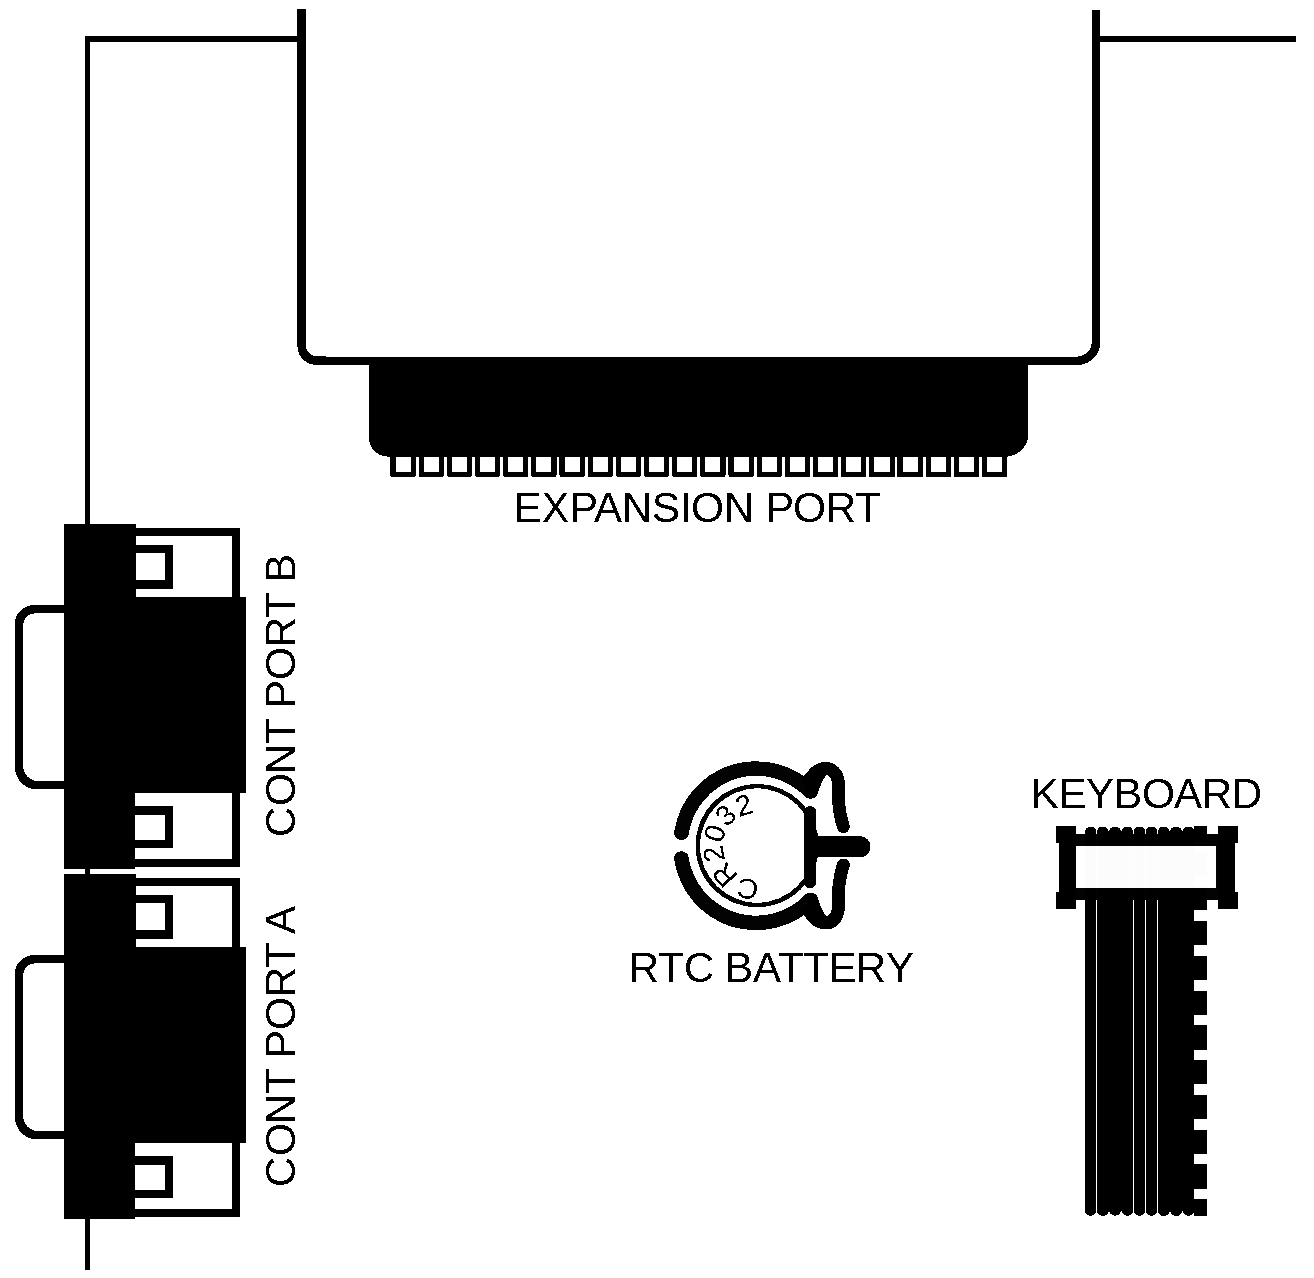
\includegraphics[width=\linewidth]{images/illustrations/rtc-battery-location.pdf}

If you are removing an existing battery, push the battery release lever on the bottom (flat-sided) side of the battery socket away from the battery to remove it. Insert the new battery with the side labelled {\bf +} facing up, and press it into place.

Once you have re-assembled your MEGA65, you can set the time in the Configuration Utility. For more information on how to set the Real-Time Clock, refer to the Configuration Utility section on page \pageref{sec:configuration-utility}.


\newpage

\section{Switching the MEGA65 on for the First Time}
\label{onboarding}

Switch the MEGA65 on using the power switch on the left-hand side of the computer.

When you switch your MEGA65 on for the first time, it displays the initial configuration (``on-boarding'') screen.\index{Configuration!On-boarding} You can use this screen to set the time and date on the Real-Time Clock (if you have installed the CR2032 battery), change the video display mode, and test the audio. All of these settings can be changed later.

\begin{center}
  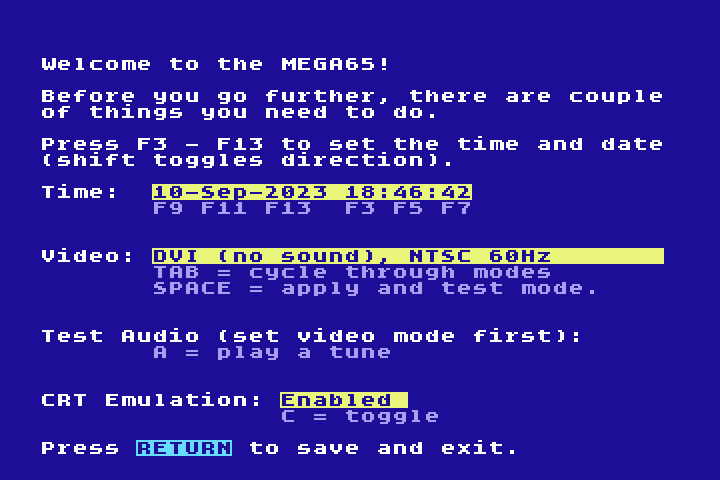
\includegraphics[width=0.7\linewidth]{images/img011_final_boot_01.png}
\end{center}

For video display modes, you can select between PAL\index{PAL display mode} or NTSC\index{NTSC display mode} emulation, and you can select whether your Digital Video display supports sound. If you are using the VGA video output, the Digital Video sound mode has no effect.

\underline{NOTE}: A DVI display that does not support sound will not work with the ``enhanced'' sound mode. With such a display, you must select a video mode with ``no sound,'' and connect a speaker to the 3.5 mm audio jack.

PAL and NTSC are analog video signal formats that affect the resolution and vertical sync speed of the video output, even when using a modern digital display. Your display may support either mode, or it may only support one or the other. You can use this screen to test the modes with your display.

Select and test your video configuration. For example, press \specialkey{TAB} to switch to the {\bf PAL 50HZ} mode.
\index{Display!Setting PAL/NTSC}
\begin{center}
  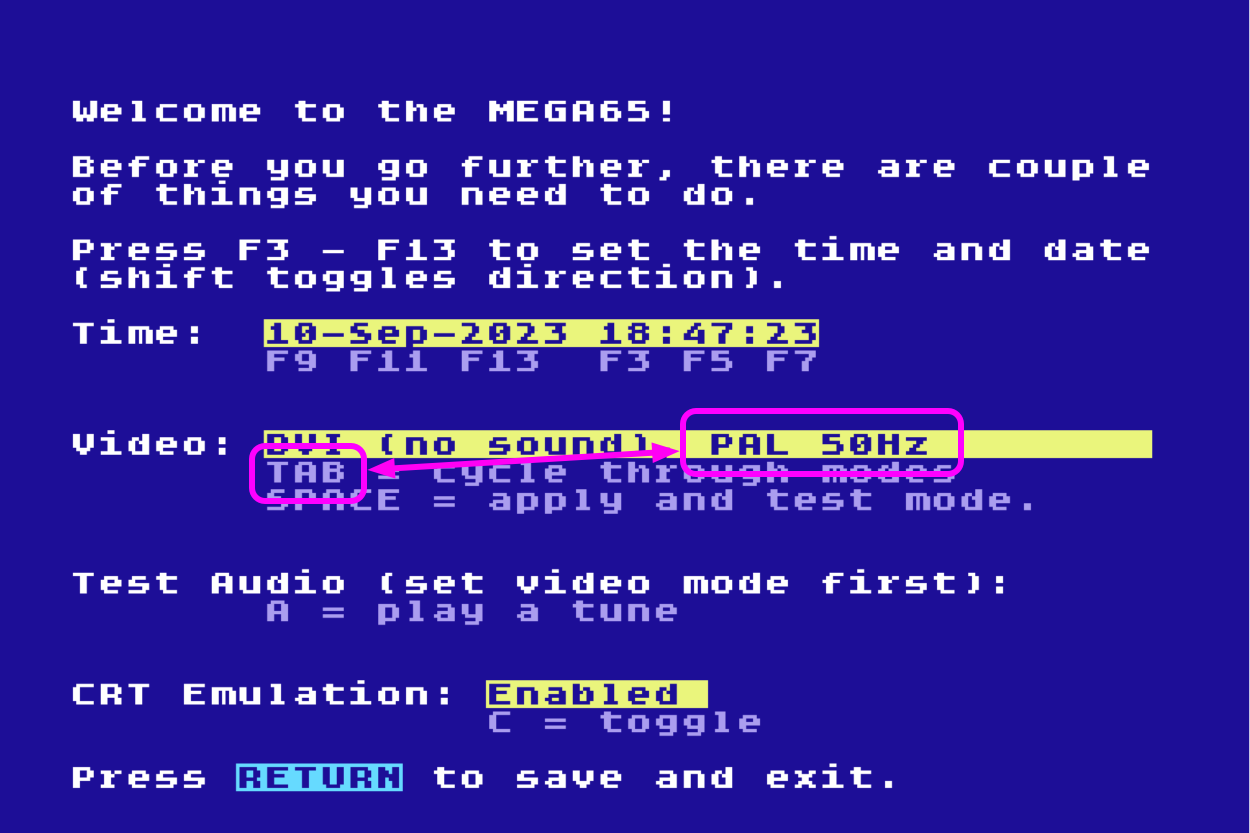
\includegraphics[width=0.7\linewidth]{images/img011_final_boot_02.png}
\end{center}

Press \megakey{SPACE} followed by \megakey{Y} to test the new video mode.

\begin{center}
  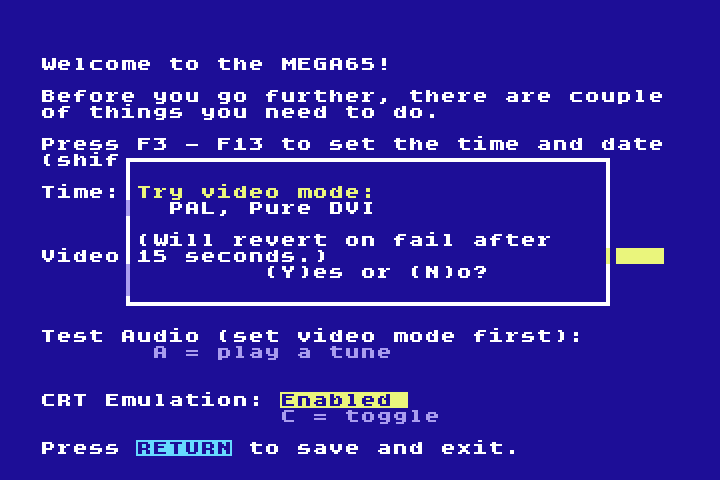
\includegraphics[width=0.7\linewidth]{images/img011_final_boot_03.png}
\end{center}

Press \megakey{K} to keep the new video mode.

\begin{center}
  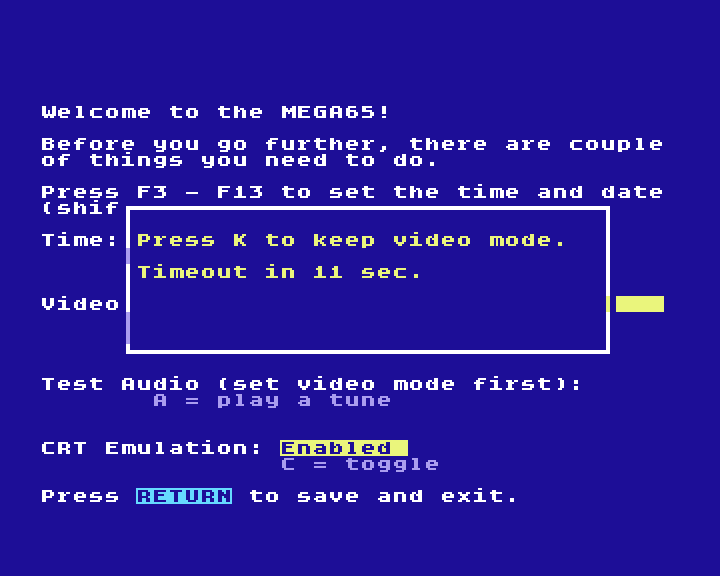
\includegraphics[width=0.7\linewidth]{images/img011_final_boot_04.png}
\end{center}

Take this opportunity to test your sound set-up. Press \megakey{A} to play a sound.

The ``CRT emulation'' option is a fun choice when using a modern flat panel display. It adds vertical gaps between pixels to simulate the CRT raster line. Try it to see if you like it: press the \megakey{C} key to toggle it on and off.

Finally, press \specialkey{RETURN} to complete the configuration.

For more information about configuring your MEGA65, see chapter \vref{cha:configuringyourmega}.

\section{The Intro Disk}
\index{Intro Disk}

After completing the on-boarding configuration, your MEGA65 starts the Intro Disk menu. The Intro Disk is a collection of software made by the MEGA65 community that demonstrates some of the capabilities of the computer. Take some time to browse the menus and try some of the demos. After each demo, press the reset button on the left-hand side of the computer to return to the Intro Disk menu.

\begin{center}
  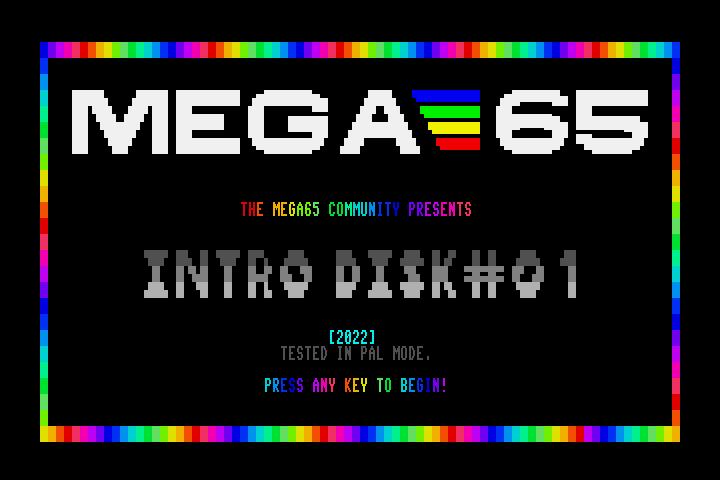
\includegraphics[width=0.7\linewidth]{images/demo_title.png}
\end{center}

By default, the Intro Disk menu opens each time you switch on the computer. Once you are more familiar with the MEGA65, you may wish to disable this. Press \megakey{D} at the Intro Disk menu to disable its auto-boot feature.\index{Intro Disk!Disabling}

Press \megakey{X} to exit the Intro Disk menu and access BASIC 65. With the Intro Disk auto-boot feature disabled, the MEGA65 goes directly to BASIC 65 when you switch it on.

\begin{center}
  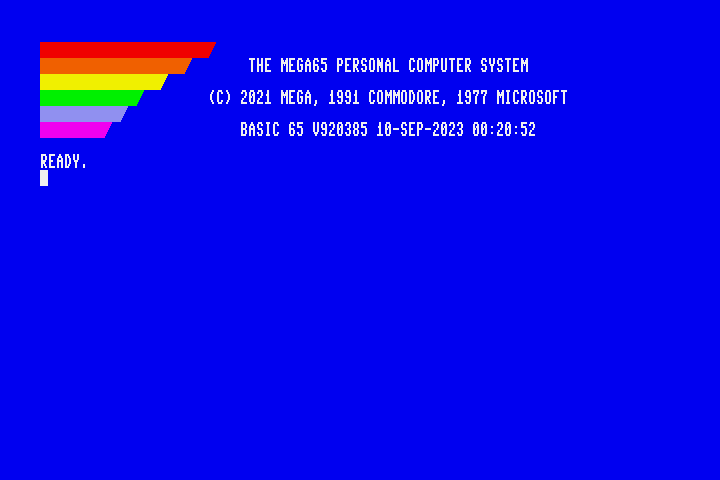
\includegraphics[width=0.7\linewidth]{images/img011_final_boot_06.png}
\end{center}

\section{The Cursor}

The flashing square underneath the \screentext{READY} prompt\index{READY prompt} is called the cursor. The cursor indicates that the computer is ready to accept input. Pressing keys on the keyboard will print their respective characters onto the screen. The characters will be printed at the current cursor position, and the cursor will advance to the next position after every key press.

Here you can type commands, that can do things such as loading a program. You can also start entering program code!

\chapter{Getting Started}
\addtocontents{toc}{\protect\setcounter{tocdepth}{2}}
\hypersetup{bookmarksdepth=5}

\section{Keyboard}
\label{cha:getting-started}
\index{Keyboard}

Now that everything is connected, it's time to get familiar with the MEGA65 keyboard.

You may notice that the keyboard is a little different to the keyboards used on other computers today. While most keys will be in familiar positions, there are some specialised keys, and some with special graphic symbols marked on the front.

The graphic symbols are typable in some display modes, similar to letters, numbers, and punctuation. The complete set of characters is known as the {\em PETSCII character set}.\index{PETSCII}

\subsection{Special Keys}

\subsubsection{RETURN}
\index{Keyboard!RETURN}
Pressing \specialkey{RETURN} enters the information you have typed into the MEGA65's memory. The computer will either act on a command, store some information, or display an error message if you made a mistake.

\subsubsection{SHIFT}
\index{Keyboard!Shift Keys}
The two \specialkey{SHIFT} keys are located on the left and the right. They work very much like the Shift key on a regular keyboard. They also perform some special functions as well.

In upper case mode, holding down \specialkey{SHIFT} and pressing any key with two graphic symbols on the front produces the right-hand symbol on that key. For example, \specialkey{SHIFT} and \megakey{J} prints the \graphicsymbol{J} character.

In lower case mode, pressing \specialkey{SHIFT} and a letter key prints the upper case letter on that key.

To type the Greek letter $\pi$ (pi), hold \specialkey{SHIFT} and press \megakeywhite{$\uparrow$}.

Holding \specialkey{SHIFT} down and pressing a Function key accesses the function shown on the front of that key. For example: \specialkey{SHIFT} and \megakey{F1} activates \megakey{F2}.


\subsubsection{SHIFT LOCK}
\index{Keyboard!SHIFT LOCK}
In addition to \specialkey{SHIFT} is \specialkey{SHIFT\\LOCK}. Press this key to lock down the Shift function. Now any key you press while \specialkey{SHIFT\\LOCK} is illuminated prints the character to the screen as if you were holding down \specialkey{SHIFT}. This includes special graphic characters.

\subsubsection{CTRL}
\index{Keyboard!CTRL}
\specialkey{CTRL} is the Control key. Holding down \specialkey{CTRL} and pressing another key allows you to perform Control functions. For example, holding down \specialkey{CTRL} and one of the number keys (from \megakey{1} to \megakey{8}) allows you to change text colours. The colour that is printed at the top row on the front of the number key will be used. Holding down \specialkey{CTRL} and pressing \megakey{9} or \megakey{0} switches reverse-text mode on and off.

There are some examples of this on page \pageref{sec:screen-editor}, and all of the Control functions are listed on page \pageref{appendix:controlcodes}.

If a program is being {\bf LIST}ed to the screen, holding down \specialkey{CTRL} slows down the display of each line. You can read more about the {\bf LIST} command on page \pageref{BASIC 65 Commands!LIST}.\index{BASIC 65 Commands!LIST}

Holding \specialkey{CTRL} and pressing \megakey{*} enters the Matrix Mode Debugger (refer to the {\bf MEGA65 Book} for more details).

\subsubsection{RUN/STOP}
\index{Keyboard!RUN STOP}
Normally, pressing \specialkey{RUN\\STOP} stops the execution of a program. Holding \specialkey{SHIFT} while pressing \specialkey{RUN\\STOP} {\bf RUN}s the first program from disk.\index{BASIC 65 Commands!RUN}

Some programs override the \specialkey{RUN\\STOP} key and cannot be stopped in this way.

You can boot your MEGA65 into the {\bf Machine Code Monitor}\index{Machine Code Monitor} by holding down \specialkey{RUN\\STOP} and pressing reset (or while switching on the computer) on the left-hand side of the computer.

\subsubsection{RESTORE}
\index{Keyboard!RESTORE}
The computer screen can be restored to a clean state without clearing the memory by holding down \specialkey{RUN\\STOP} and pressing \widekey{RESTORE}. This combination also resets operating system vectors and re-initialises the screen editor, which makes it a handy combination if the computer has become a little confused.

Some programs override the \specialkey{RUN\\STOP} + \widekey{RESTORE} key combination and cannot be reset in this way.

You can also enter the {\bf Freezer} by pressing and holding \widekey{RESTORE} for one second, then releasing the key. You can
read more about the Freezer on page \pageref{sec:freezer}.\index{Freezer menu}

\subsubsection{THE CURSOR KEYS}
\index{Keyboard!Cursor Keys}
\nopagebreak
At the bottom right-hand side of the keyboard are the cursor keys. These four directional keys allow you move the cursor to any position for on-screen editing.

The cursor moves in the direction indicated on the keys: \megakey{$\leftarrow$} \megakey{$\uparrow$} \megakey{$\rightarrow$} \megakey{$\downarrow$}.

You don't have to keep pressing a cursor key over and over. If you need to move the cursor a long way, you can keep the key pressed down. When you are finished, simply release the key.

\subsubsection{ARROW KEYS}
\index{Keyboard!Arrow Keys}
These keys are different to the cursor keys! They are \megakeywhite{$\leftarrow$} (next to \megakey{1}), and \megakeywhite{$\uparrow$} (next to \widekey{RESTORE}).
Both arrow keys are used in various BASIC functions and escape sequences.

For example, \megakeywhite{$\leftarrow$} can be used as a shortcut for {\bf SAVE},\index{BASIC 65 Commands!SAVE} and \megakeywhite{$\uparrow$} is used to raise a number to a power (which is the same as multiplying a number by itself a specified number of times).

You can read more about the available escape sequences on page \pageref{escape-sequences}.

These two PETSCII specific keys will always be shown in MEGA65 literature with a white background.

It is also possible to move the cursor up by using \specialkey{SHIFT} and \megakey{$\downarrow$}, and left by using \specialkey{SHIFT} and \megakey{$\rightarrow$}. This owes to the MEGA65's Commodore 64 heritage, which only had two cursor keys.

\subsubsection{INSerT/DELete}
\index{Keyboard!INST DEL}
The \specialkey{INST\\DEL} key, the rightmost key of the top row, is the INSERT / DELETE key. When you press \specialkey{INST\\DEL}, the character to the left is deleted, and all characters to the right are shifted one position to the left.

To insert a character, hold \specialkey{SHIFT} and press \specialkey{INST\\DEL}. The character under as well as the characters to the right of the cursor are shifted to the right. This allows you to type a letter, number or any other character at the newly inserted space.


\subsubsection{CLeaR/HOME}
\index{Keyboard!CLR HOME}
The \specialkey{CLR\\HOME} is the CLEAR / HOME key. Pressing \specialkey{CLR\\HOME} places the cursor at the top left-most position of the screen.

Holding down \specialkey{SHIFT} and pressing \specialkey{CLR\\HOME} clears the entire screen {\it and} places the cursor at the top left-most position of the screen.

If you press \specialkey{CLR\\HOME} accidentally, you can return the cursor to its prior position by pressing \specialkey{ESC} then \specialkey{CLR\\HOME}.

\subsubsection{MEGA KEY}
\index{Keyboard!MEGA Key}
\megasymbolkey or the MEGA key provides a number of different functions and can be used to launch special utilities.

Holding \specialkey{SHIFT} and pressing \megasymbolkey switches between lower and uppercase character modes.

Holding \megasymbolkey and pressing any key with two graphic symbols on the front prints the left-most graphic symbol to the screen. For example,
\megasymbolkey and \megakey{D} prints the \graphicsymbol{d} symbol.

Holding \megasymbolkey and pressing a number key switches to a secondary colour, i.e., the colour that is printed at the bottom row on the front of the number key.

Holding \megasymbolkey and pressing \specialkey{TAB} enters the Matrix Mode Debugger (refer to the {\bf MEGA65 Book} for more details).

Switching on the MEGA65 or pressing the reset button on the left-hand side while holding down \megasymbolkey switches the MEGA65 into GO64 mode.\index{Commodore 64!GO64 mode}

\subsubsection{NO SCROLL}
\index{Keyboard!NO SCROLL}
If a program is being {\bf LIST}ed to the screen, pressing \specialkey{NO\\SCROLL} pauses the screen output. Press any key to un-pause.

This feature is not available in GO64 mode.\index{Commodore 64!GO64 mode}

\subsubsection{FUNCTION KEYS}
\index{Keyboard!Function Keys}
There are seven Function keys available for use by software applications. \megakey{F1} \megakey{F3} \megakey{F5} \megakey{F7} \megakey{F9} \megakey{F11} and \megakey{F13} can be used to perform special functions.

Hold \specialkey{SHIFT} to access \megakey{F2} through to \megakey{F14} as shown on the front of each Function key.
\index{Keyboard!Shift Keys}
Only Function keys \megakey{F1} to \megakey{F8} are available in GO64 mode.\index{Commodore 64!GO64 mode}

\subsubsection{HELP}
\index{Keyboard!HELP}
\specialkey{HELP} can be used by software, and also acts as \megakey{F15}.

\subsubsection{ALT}
\index{Keyboard!ALT}
Holding \specialkey{ALT} down while pressing other keys can be used by software to perform specific functions. This feature is not available in GO64 mode.\index{Commodore 64!GO64 mode}

Holding \specialkey{ALT} down while switching the MEGA65 on activates the Utility Menu.\index{Utility menu} You can format an SD card, or enter the MEGA65 Configuration Utility\index{Configuration!Utility} to select the default video mode and change other settings, or test your keyboard.

\subsubsection{CAPS LOCK}
\index{Keyboard!CAPS LOCK}
\specialkey{CAPS\\LOCK} works similarly to \specialkey{SHIFT\\LOCK} in C65 and MEGA65-modes, but only modifies the letter keys.

When the MEGA65 is set to run at a reduced processor speed, such as in GO64 mode,\index{Commodore 64!GO64 mode} you can hold down \specialkey{CAPS\\LOCK} to run the processor at full speed temporarily. This is useful in GO64 mode for things such as
speeding up loading from the internal disk drive or SD card, or to greatly speed up the de-packing process after a program is run. MEGA65 mode runs at maximum speed by default.

\addtocontents{toc}{\protect\setcounter{tocdepth}{5}}


\section{The Screen Editor}
\label{sec:screen-editor}

When you switch on your MEGA65 or reset it, the following screen will appear:\footnote{This assumes you have disabled the Intro Disk menu. If the Intro Disk menu is running, press ``/'' (forward slash) to exit to this screen.}

\begin{center}
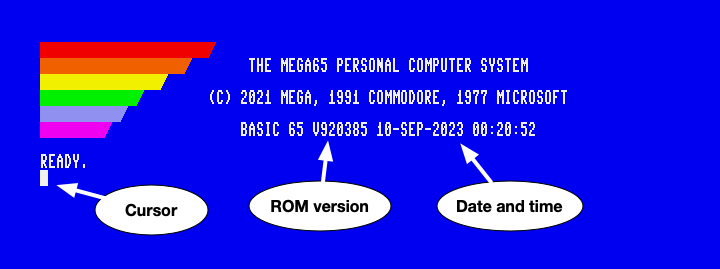
\includegraphics[width=0.9\linewidth]{images/introduction-screen/layout.png}
\end{center}

The colour bars in the top left-hand side of the screen can be used as a guide to help calibrate the colours of your display. The screen also displays the name of the system, the copyright notice, and the ROM version. The displayed date and time are taken from the internal RTC (Real-Time Clock) at the time the computer was powered on. You can set the date and time in the Configuration Utility.

Finally, you will see the \screentext{READY} prompt and the flashing cursor.

You can begin typing keys on the keyboard and the characters will be printed at the cursor position. The cursor itself will advance after each key press.

You can also produce reverse text or colour bars by holding down \specialkey{CTRL} and pressing \megakey{9}, or \megakey{R}. This enters reverse text mode. When this is enabled, you can press and hold the \megakey{Space} bar. While doing so, a white bar will be drawn across the screen.
\index{Keyboard!CTRL}
You can change the current colour by holding \specialkey{CTRL} down and pressing a number key (from \megakey{1}
to \megakey{8}). For example, if you press and hold \specialkey{CTRL} down and press \megakey{1}, the colour will
change to black. Now, when you hold down the \megakey{Space} bar, a black bar will be drawn. If you continue to
change the colour and press the \megakey{Space} bar, you will get an effect similar to the following image:

\begin{center}
\includegraphics[width=0.7\linewidth]{images/introduction-screen/colour-bars.png}
\end{center}

You can disable reverse text mode by holding \specialkey{CTRL} and pressing \megakey{0}.

A further eight colours can be selected by holding down \megasymbolkey and pressing a key from \megakey{1} to \megakey{8}.\index{Keyboard!MEGA Key}

The colour that is printed at the bottom row on the front of the number key will be used. For example, if you held
\megasymbolkey down while pressing \megakey{4}, dark grey will be used. For access to an additional 16 colours of the alternate/rainbow palette, refer to the \specialkey{CTRL} + \megakey{A} shortcut described on page \pageref{appendix:controlcodes}.

\underline{NOTE}:
\begin{itemize}
  \item {\bf Quote Mode}: If you were to press \megakey{"} to open a string, and then try to change
colours, reverse text, move the cursor keys, or use the \specialkey{CLR\\HOME} key, instead
of these actions instantly occurring, funny PETSCII\index{PETSCII} symbols will appear instead. This is
due to a BASIC facility called {\it quote mode},
which allows you to encode such actions into a string so that they can be executed at a later
time (for example, via a {\bf PRINT} statement within your programs). To end quote mode, simply
type another \megakey{"} to mark the end of your string.
  \item {\bf Insert Mode}: A similar facility is called
{\it insert mode}, where for the number of times you press \specialkey{SHIFT} + \specialkey{INST\\DEL}
to insert a few spaces, the same number of keypresses that follow it will abide by the same
principles of quote mode.
  \item You can forcefully exit either of these modes by pressing \specialkey{ESC}, \megakey{O}.
\end{itemize}

\needspace{4cm}
You can create fun pictures just by using these colours and letters. Here's an example of what a 4th year student drew:

\begin{center}
\includegraphics[width=0.7\linewidth]{images/caleb-PETSCII-TNT-final}
\end{center}

What will you draw?

\needspace{2cm}
\textbf{Functions}

Functions using \specialkey{CTRL} are called \textbf{Control Codes}.
Functions using \megasymbolkey are called \textbf{Mega Codes}. There are also functions that are called by using \specialkey{SHIFT}, which are called \textbf{Shifted Codes}.

Lastly, \specialkey{ESC} enables the use of \textbf{Escape Sequences}.

You can read about all of these functions in detail on page \pageref{appendix:controlcodes}.

\needspace{2cm}
\textbf{ESC Sequences}

\index{Keyboard!Escape Sequences}
Escape sequences are performed a little differently than a Control function or a Shift function. Instead of holding the modifier key down, an Escape sequence is performed by pressing \specialkey{ESC} and releasing it, followed by pressing the desired key.

For example, to switch between 80 column mode and 40 column mode, press and release \specialkey{ESC}, then press \megakey{X}.

There are more text modes available. You can create flashing text by holding \specialkey{CTRL} down and pressing \megakey{O}. Any characters you type in will flash. Turn flash mode off by pressing \specialkey{ESC}, then \megakey{O}.


\section{Editor Functionality}

The MEGA65 screen editor\index{Screen editor} supports several ways to quickly move the cursor around the screen to help you to be more productive.

For example, press \specialkey{CLR\\HOME} to go to the home position on the screen. Hold \specialkey{CTRL} down and press \megakey{W} several times. This is the \textbf{Word Advance function}, which jumps your cursor to the next word, or printable character.

You can set custom tab positions on the screen for your convenience. Press \specialkey{CLR\\HOME} and then \megakey{$\rightarrow$} to move the cursor to the fourth column. Hold down \specialkey{CTRL} and press \megakey{X} to set a tab. Move another 16 positions to the right, and press \specialkey{CTRL} and \megakey{X} again to set a second tab.

Press \specialkey{CLR\\HOME} to go back to the home position. Hold \specialkey{CTRL} down and press \megakey{I}. This is the \textbf{Forward Tab function}. Your cursor will tab to the fourth position. Press \specialkey{CTRL} and \megakey{I} again. Your cursor will move to position 8. By default, every 8th position is already set as a tabbed position. So the 4th and 20th positions have been added to the existing tab positions. You can continue to press \specialkey{CTRL} and \megakey{I} to advance to the 16th and 20th positions.

\subsection{Creating a Window}
\index{Keyboard!Escape Sequences}
\index{Windows!Escape sequences}

You can set a window on the MEGA65 working screen. Move your cursor to the beginning of the "BASIC 65" text. Press \specialkey{ESC}, then press \megakey{T}. Move the cursor 10 lines down and 15 to the right.

Press \specialkey{ESC}, then \megakey{B}. Anything you type will be contained within this window.

For example, if you were to type \screentext{LIST} to list out a program, the listing will be confined to the window region you have specified:

\begin{center}
\includegraphics[width=0.7\linewidth]{images/set-window.png}
\end{center}

To escape from the window back to the full screen, press \specialkey{CLR\\HOME} twice.

\subsection{Additional ASCII characters}

You may have noticed a few ASCII characters on the MEGA65 keyboard that aren't traditionally a part of the PETSCII character set\index{PETSCII}. To use these characters:

\begin{itemize}
  \item Type either \screentext{FONT A} or \screentext{FONT B}.
  \item Press \megasymbolkey + \specialkey{SHIFT} to switch to lowercase.
\end{itemize}

You will now be able to type those additional ASCII characters by holding \megasymbolkey and pressing the key.

\begin{center}
  \begin{tabular}{|l|c|l|}
  \hline
  \textbf{Name} & \textbf{Symbol} & \textbf{Key} \\
  \hline
  Backtick & \texttt{\`} & \megasymbolkey + \megakeywhite{$\leftarrow$} \\
  \hline
  Tilde & \texttt{\~} & \megasymbolkey + \megakey{,} (comma) \\
  \hline
  Vertical bar & \texttt{|} & \megasymbolkey + \megakey{.} (period) \\
  \hline
  Backslash & \texttt{\textbackslash} & \megasymbolkey + \megakey{/} \\
  \hline
  Left curly bracket & \texttt{\{} & \megasymbolkey + \megakey{:} \\
  \hline
  Right curly bracket & \texttt{\}} & \megasymbolkey + \megakey{;} \\
  \hline
  Underscore & \texttt{\_} & \megasymbolkey + \megakey{=} \\
  \hline
  \end{tabular}
\end{center}

The alternate fonts replace characters from the original PETSCII character set with these symbols. To revert back to the PETSCII character set, type \screentext{FONT C}.

\subsection{Uppercase and lowercase}

\megasymbolkey + \specialkey{SHIFT} switches between uppercase and lowercase text for the entire display. This works even during program execution, so you can adjust it if a program is in the wrong mode.


\section{The Freezer Menu}
\label{sec:freezer}
\index{Freezer menu}
\nopagebreak
The MEGA65 spends most of its time behaving as a Commodore 65 computer would, either running a program or awaiting instructions in the BASIC environment. Your MEGA65 has additional features that were not part of the original C65 design. You can access many of these features from the Freezer menu.

To open the Freezer menu, hold the \widekey{RESTORE} key for one second, then release it. The MEGA65 will pause whatever it is doing, flicker the border colour, then open the Freezer menu. Whatever program was running remains in memory and can be resumed by pressing the \megakey{F3} key. You can also abandon the running program and reset the MEGA65 by pressing \megakey{F5}.

\begin{center}
  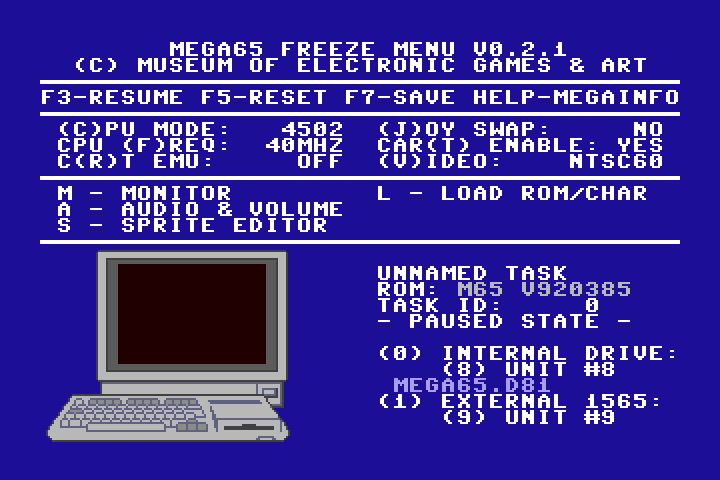
\includegraphics[width=0.7\linewidth]{images/freezer.png}
\end{center}

One feature to remember when playing games is the ``(J)OY SWAP.'' This causes the two joystick ports to trade numbers. If you have a joystick in port 2 and you start a game that expects a joystick in port 1, instead of disconnecting and reconnecting the joystick, open the Freezer menu, press \megakey{J} to swap the port numbers, then resume your game.

This is called the ``Freezer'' menu because the state of the MEGA65 remains frozen while using it. The Freezer menu can store multiple freeze states, and you can switch between them. To save the current state, navigate to an unused {\it freeze slot} using the cursor-right key, then press \megakey{F7}. When the border stops blinking, the state is saved. To restore a state, navigate to the freeze slot, then press \megakey{F3} to resume operation.

The Freezer menu has several built-in options and features. For more information about the MEGA65 Information Utility (``MEGAINFO''), see ``Determining the Versions of Things'' on page \pageref{sec:versions}. For more information about mounting disks and disk images, see chapter \vref{cha:using-disks}.


\section{Running Commodore 64 Software}

The MEGA65 is capable of running Commodore 64 software. There are two ways to do this: the built-in GO64 mode, and the {\it C64 for MEGA65} FPGA core.

\subsection{GO64 Mode}
\index{Commodore 64!GO64 mode}

The original Commodore 65 was designed to be capable of running some Commodore 64 software. The MEGA65 supports this feature, known as ``GO64 mode.''

\underline{NOTE}: Due to how Commodore designed this feature, not all C64 software is compatible with this mode. Unlike the similar feature of the Commodore 128, the Commodore 65 uses a different CPU, and minor differences are known to cause compatibility issues with some software titles.

There are three ways to switch the MEGA65 into GO64 mode:

\begin{itemize}
    \item Switch off the computer, hold the \megasymbolkey and switch it back on.
    \item From the MEGA65 \screentext{READY} prompt, enter this command: \screentext{GO64} Enter \screentext{YES} when prompted.\index{BASIC 65 Commands!GO64}
    \item Switch off the computer, connect a Commodore 64 cartridge to the expansion port, then switch the computer on.
\end{itemize}

\begin{center}
  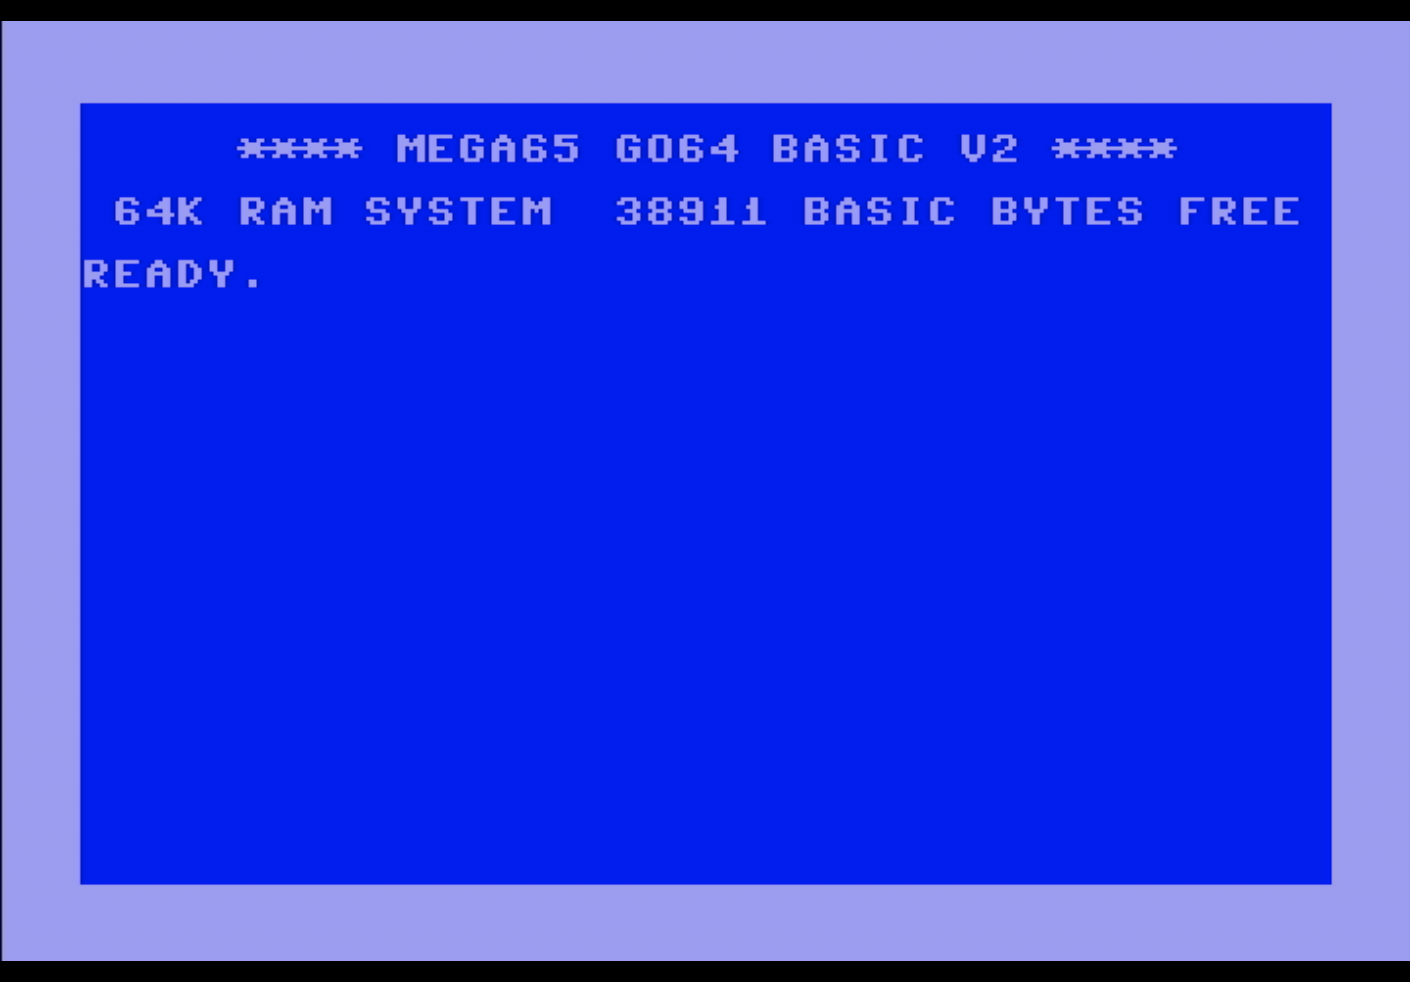
\includegraphics[width=0.7\linewidth]{images/go64.png}
\end{center}

GO64 mode is actually just a temporary re-configuration of the MEGA65. All of the MEGA65's features are still present, including the Freezer menu for mounting D81 disk images.

Much Commodore 64 software can be found on the Internet in the form of D64 disk images. The MEGA65 only supports D81 disk images via the SD card and Freezer menu. You can use a peripheral such as the SD2IEC\index{SD2IEC device} with the MEGA65's IEC port to use D64 disk images. Be sure to obtain an SD2IEC with an independent power supply, and not one that depends on a Commodore 64 tape connector.\footnote{For more information on SD2IEC devices, see: \url{https://www.c64-wiki.com/wiki/SD2IEC}}

\subsection{The ``C64 for MEGA65'' FPGA Core}
\index{Core!C64 core}\index{Commodore 64!Core}

The {\it C64 for MEGA65} FPGA core by MJoergen and sy2002 re-creates the original Commodore 64 computer on MEGA65 hardware with a high degree of accuracy. It does so by completely replacing the MEGA65 core with one that implements the Commodore 64 chipset, including its CPU. MEGA65 features such as the Freezer menu are not available when running the C64 core. Instead, the core provides its own menu for mounting D64 disk images and other features. Press the \specialkey{HELP} key with the core running to access this menu.

% TODO: When the cartridge-to-core configuration feature is complete:
% With the C64 core installed, you can configure the MEGA65 boot process to use the core when a Commodore 64 cartridge is connected, instead of using the less-compatible GO64 mode. ...
% (Refer to chapter \vref{cha:cores})

For information about installing FPGA cores, see chapter \vref{cha:cores}. To download the {\it C64 for MEGA65} core and read important installation instructions, see: \url{https://github.com/MJoergen/C64MEGA65}

\chapter{Configuring Your MEGA65}

\section{Configuring Your MEGA65}
\label{cha:configuringyourmega}
\index{Configuration}

This chapter describes how to configure your MEGA65.

Configuration data is stored on the SD card, so this chapter also describes how to prepare a new SD card. Your MEGA65 comes with an SD card pre-installed. If you configure your MEGA65 using the pre-installed SD card then later install a new SD or microSD card, you will need to set your configuration settings again.

This chapter also introduces the MEGA65 Filehost website, which you can use to download games, apps, tools, and system updates for your computer.

\section{The Configuration Utility}
\label{sec:configuration-utility}
\index{Configuration!Utility}

You can configure your MEGA65 using the Configuration Utility. This includes the settings shown when you switched on the machine for the first time, and many others.

To access the Configuration Utility, switch off the MEGA65, hold the \specialkey{ALT} key and switch it back on. The Utility menu\index{Utility menu} appears with several options. Press \megakey{1} to start the Configuration Utility.

\begin{center}
  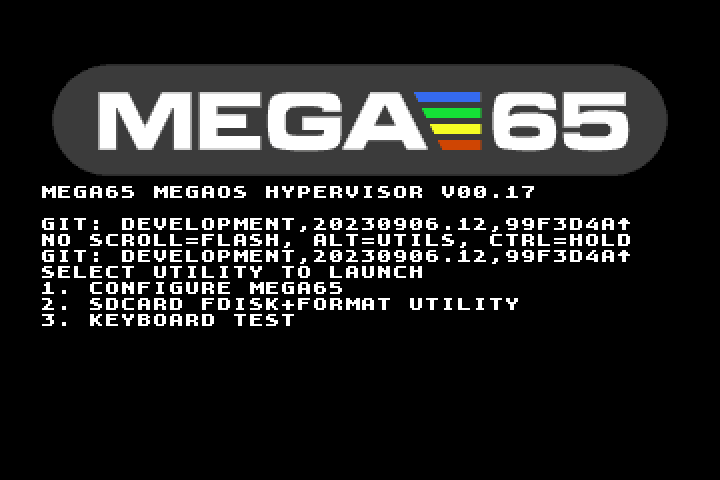
\includegraphics[width=0.7\linewidth]{images/ss-utilmenu.png}
\end{center}

The Configuration Utility includes several pages of settings, which you can navigate using the keyboard or a mouse connected to port 1. Use \megakey{$\leftarrow$} and \megakey{$\rightarrow$} to navigate between pages, and \megakey{$\uparrow$} and \megakey{$\downarrow$} to select items on the page. Press \specialkey{RETURN} or \megakey{SPACE} to toggle a setting or change a value.

\subsection{Input}
\index{Configuration!Mouse}

The {\bf Input} page configures the mouse settings for the two peripheral ports.

\begin{center}
  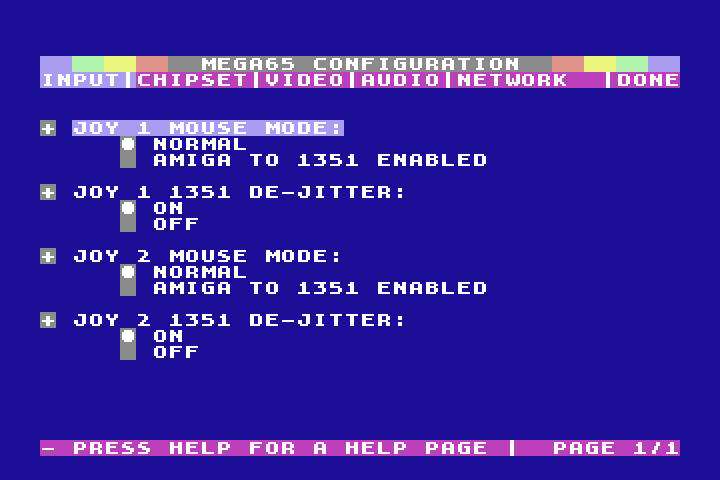
\includegraphics[width=0.7\linewidth]{images/ss-m65config-1.png}
\end{center}

The MEGA65 supports the Commodore 1351 mouse,\index{Commodore 1351 mouse} the Commodore Amiga mouse,\index{Commodore Amiga mouse} or modern equivalents such as a USB mouse connected with a \href{https://retrohax.net/shop/amiga/mouster/}{mouSTer} adapter.\index{mouSTer adapter} The port must be set to the correct mouse type, where {\bf normal} refers to the 1351 mouse. If an Amiga mouse is connected while the port is in the {\bf normal} mode, it may interfere with the behavior of the keyboard.

The {\bf 1351 De-jitter} setting adjusts the sensitivity in Commodore 1351 mouse mode to avoid jitter in the mouse pointer. It is recommended to leave this set to {\bf on} when using a 1351 mouse in {\bf normal} mode.

\subsection{Chipset}
\index{Configuration!Boot Disk}

The {\bf Chipset} page configures several features, including the Real-Time Clock.

\begin{center}
  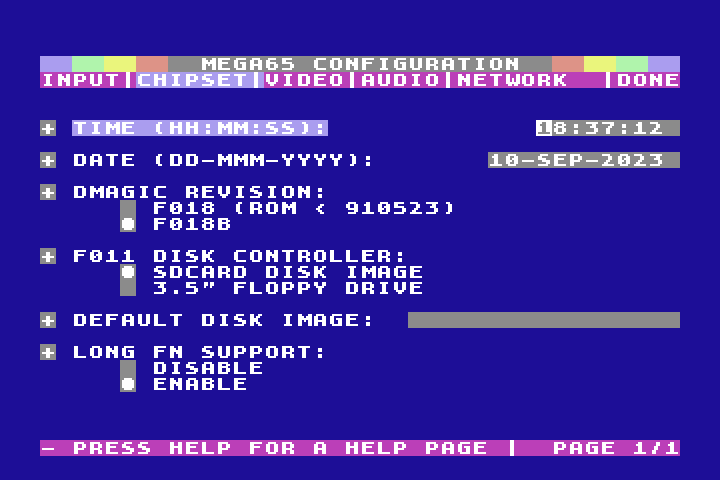
\includegraphics[width=0.7\linewidth]{images/ss-m65config-2.png}
\end{center}

To set the Real-Time Clock, select the time or date field, type the complete value, then press \specialkey{RETURN}.\index{Real-Time Clock!Setting the Date/Time}\index{Configuration!Real-Time Clock} The clock setting takes effect as soon as you press \specialkey{RETURN}, and does not take effect unless you press \specialkey{RETURN}. Note that all other settings are not saved until the end. Only the RTC is updated immediately.

The {\bf DMAGIC revision} field controls the behavior of the DMA controller. In most cases, you want the newer {\bf F018B} setting. The {\bf F018} setting is for backwards compatibility when running the C65 versions of the ROM, and is not always required.

The {\bf F011 disk controller}\index{F011 Disk Controller} field determines whether the MEGA65 looks for a boot disk on the SD card or in the physical 3.5" floppy drive when the computer is switched on.\index{Configuration!Boot Disk} When set to {\bf SDCARD disk image,} the MEGA65 uses the D81 virtual disk image named in the {\bf default disk image} field as the boot disk. When you first get your MEGA65, this is set to the Intro Disk,\index{Intro Disk} named {\tt MEGA65.D81}. You can change this to a different disk. To disable auto-mounting, change the disk name to a filename that does not exist, or rename the {\tt MEGA65.D81} file on the SD card. (Leaving the setting empty will default to {\tt MEGA65.D81}.)

If {\bf F011 disk controller} is set to {\bf 3.5" floppy drive,} the boot process will pause just before the \screentext{READY.} prompt to check if a boot disk is inserted in the drive. If you do not use a physical boot disk, you may wish to leave this set to {\bf SDCARD disk image} for a faster boot process.

{\bf Long FN support} refers to long filename support in the MEGA65 SD card file browser features. Leave this enabled unless there is an issue with reading files with filenames longer than 11 characters.

\subsection{Video}
\index{Configuration!Video}

The {\bf Video} page configures video settings. These are the same settings from the on-boarding configuration, including the PAL or NTSC video mode, Digital Video sound, and CRT emulation.\index{Configuration!On-boarding}\index{Display!Setting PAL/NTSC}

\begin{center}
  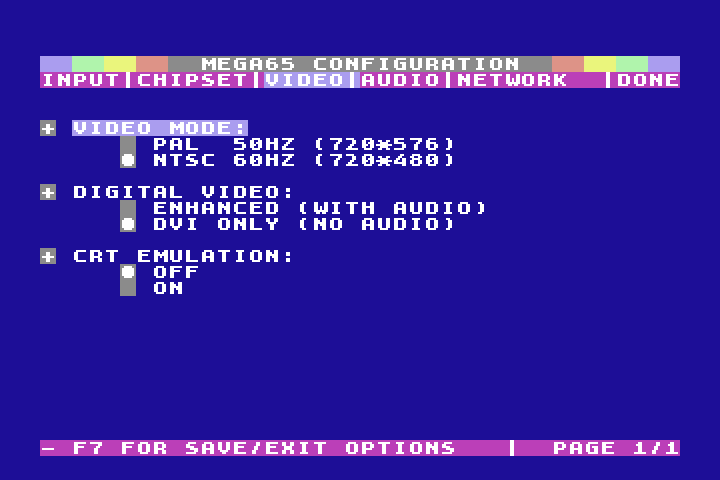
\includegraphics[width=0.7\linewidth]{images/ss-m65config-3.png}
\end{center}

{\bf Video mode} selects between the PAL compatibility mode and the NTSC compatibility mode. You can also change this while running programs using the Freezer menu.

The {\bf Digital Video} setting enables or disables the combined video and audio signal over the Digital Video port. If your Digital Video display has built-in speakers, enable this setting ({\bf Enhanced (with audio)}) to use them. Some DVI displays without built-in speakers require that this is disabled.

{\bf CRT emulation} is an optional setting that makes the picture look more like that of a vintage Cathode Ray Tube display when using a modern flat-panel display.

\subsection{Audio}
\index{Configuration!Audio}

The {\bf Audio} page configures the MEGA65 sound system.\index{Configuration!Audio} In most cases, you can leave these at their default settings.

\begin{center}
  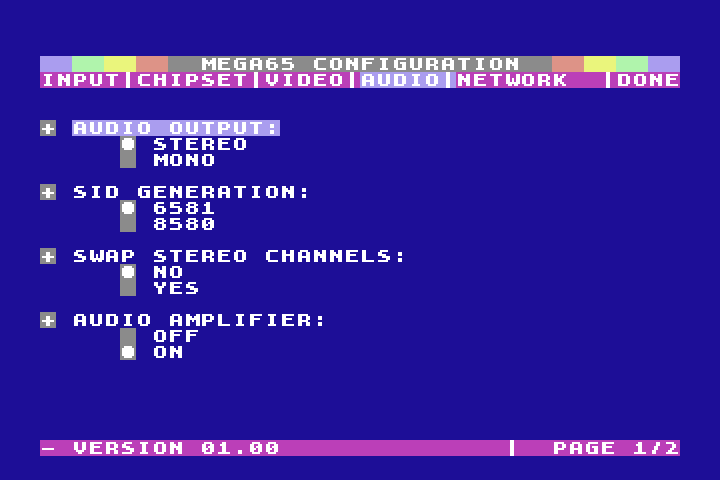
\includegraphics[width=0.7\linewidth]{images/ss-m65config-4.png}
\end{center}

{\bf Audio output} can be configured to use full stereo, or to send a monoaural signal to both speakers. When in stereo mode, various audio devices in the MEGA65 can be panned to the left or right using the audio mixer in the Freezer menu. The default settings pan the four SID chips slightly to the left and right.

{\bf SID generation} selects between the audio emulation of the two models of SID sound chips: the original 6581 used in some Commodore 64s, and the newer 8580 used in later Commodore 64s and 128s. Some Commodore 64 games took advantage of flaws in the 6581 that were fixed in the 8580, and so sound better with the older generation.

{\bf Swap stereo channels} switches the stereo mix to use the opposite speakers.

{\bf Audio amplifier} controls the built-in amplifier on the 3.5mm audio jack. Set this to {\bf on} when using headphones or another device that expects an amplified signal. Set this to {\bf off} for a line-level signal.

\subsection{Network}
\index{Configuration!Network}

The {\bf Network} page gives you the opportunity to adjust the MAC address of the Ethernet port. The MEGA65 does not have a hardware-assigned MAC address. Instead, it uses the value entered here.

If the MAC address is set to all zeros, press the \megakey{R} key to generate a random address. Networking features will not function with a MAC address set to all zeros.\index{Configuration!MAC address}\index{Networking!MAC address}

\begin{center}
  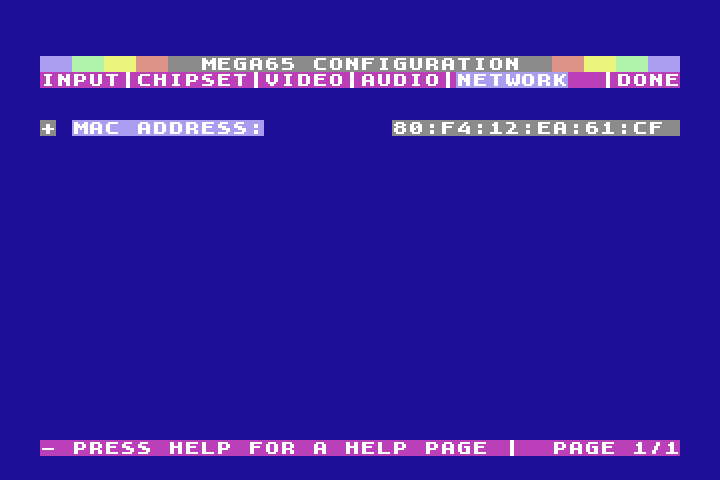
\includegraphics[width=0.7\linewidth]{images/ss-m65config-5.png}
\end{center}

\subsection{Done}

The {\bf Done} page lets you exit the Configuration Utility. If you have made changes that you want to keep, select {\bf Save as defaults and exit.} You can also abandon changes, restore the factory default settings, or completely restart to the on-boarding screen.

\begin{center}
  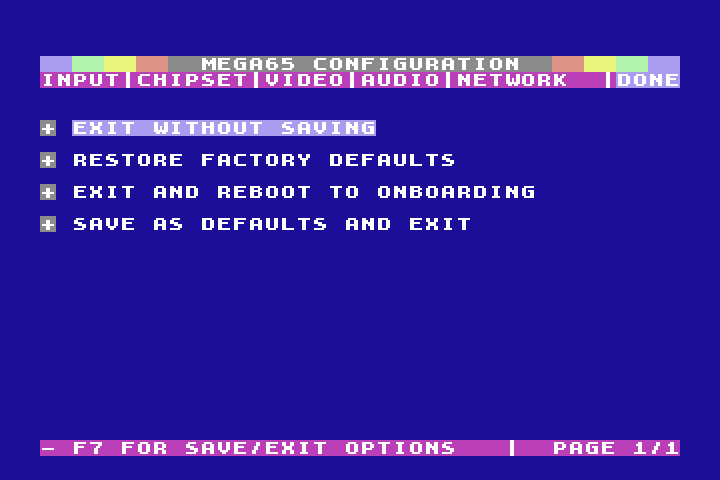
\includegraphics[width=0.7\linewidth]{images/ss-m65config-save.png}
\end{center}

When you exit the Configuration Utility, you will be prompted to ``power-cycle'' the computer. Switch the computer off, then switch it on again.

\section{Introducing SD Cards}
\label{sec:introducing-sd-cards}
\index{SD Cards}
\nopagebreak
Your MEGA65 is equipped with two SD card slots: a full-size SD card slot inside the case accessible from the bottom of the computer, and a microSD card slot accessible from the rear of the computer.\index{SD Cards!Locations} The MEGA65 uses the SD card for storing configuration settings, loading the operating system, updating the firmware, and storing your software and data as virtual disk images.

The MEGA65 includes a full-size SD card installed in the internal SD card slot, pre-populated with the operating system files and bundled software.\footnote{You can recreate the original SD card's contents using files that you can download from the Internet. Nevertheless, you may wish to make a backup of the SD card contents onto your PC.} You can connect your MEGA65 and start using it immediately without setting up a new SD card. You can leave this SD card in place and pretend that it isn't there, as if your MEGA65 is a computer from the 1990s, with a hidden ability to store non-volatile data.

The MEGA65 only uses one of the two SD card slots at one time. If there is a microSD card in the rear slot, the internal SD card is ignored. Which slot you use depends on how you expect to use the computer. As you get more familiar with your MEGA65, you may want to move the SD card between the MEGA65 and your PC to copy files and perform system updates. This is more convenient with the external microSD card slot.

Alternatively, you can connect your MEGA65 to your PC or local network with an Ethernet cable, and use a tool to transfer files between the two computers. The file transfer feature accesses files on the SD card, and uses whichever card slot is active. For more on transferring files, see chapter \vref{cha:transferring-files}.

\section{Preparing a New SD Card}

You can use the microSD memory card slot on the rear of the MEGA65 as persistent storage for the computer's configuration and system files. Having a prepared card in this slot overrides the SD card installed inside the computer. Having a microSD card installed is convenient if you wish to move it between your MEGA65 and your PC.

The following instructions apply to memory cards in either the external microSD card slot or the internal full-size SD card slot.

The MEGA65 supports SD cards of type SDHC, with sizes between 4 gigabytes and 32 gigabytes. Older cards smaller than 4GB and newer SDXC cards larger than 32GB are not expected to work.

An SD card must be prepared by the MEGA65 before use, using the SD Card Utility.\index{SD Card Utility} The utility creates two partitions: a hidden partition for configuration and freeze state data, and a FAT32-compatible partition for disk images and system files. You can access the FAT32 partition by connecting the SD card to your PC.\footnote{If you wish to make a backup of the complete SD card including the hidden partition, you must use a disk utility that copies entire partitions, not just the files on the FAT32 partition.}

An SD card formatted by another computer will {\em not} work with the MEGA65, even if it only erases the FAT32 partition. You {\em must} use the MEGA65 SD Card Utility to format the card.

\subsection{Inserting the SD Card}

Formatting an SD card erases its contents, and this operation cannot be undone. We recommend that you do not erase the internal SD card that came with the computer.

The SD Card Utility will prompt you to select which of the cards currently inserted in the computer to format. As a precaution, you may wish to remove the internal SD card before opening the SD Card Utility. You can reinstall it later, or leave it out of the machine until you need it. This is also a good opportunity to copy the bundled software files (with filenames that end in {\tt .D81}) off of the internal SD card to your PC, so they can be copied back to the new SD card later.

The utility menu is accessible even if no valid SD card is present. You can bootstrap a new system using just a compatible SD card and the SD Card Utility.

Insert the SD card that you wish to prepare before proceeding.

\subsection{The SD Card Utility}
\index{SD Card Utility}

You access the SD Card Utility from the Utility menu.\index{Utility menu} Switch off the MEGA65, hold the \specialkey{ALT} key and switch it on again. From the menu, select option \megakey{2} to start the SD Card Utility (\texttt{SDCARD FDISK+FORMAT UTILITY}).

\begin{center}
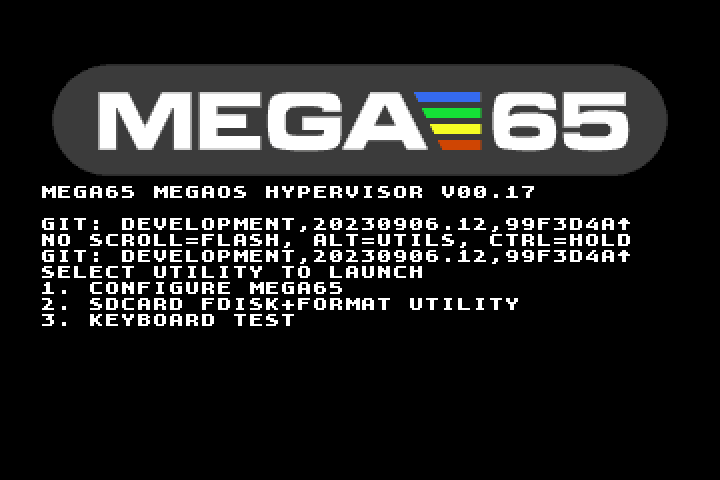
\includegraphics[width=0.7\textwidth]{images/ss-utilmenu.png}
\end{center}

The SD Card Utility opens and looks for SD cards installed in the slots. If you haven't inserted the SD card that you want to prepare yet, do so now, then press \megakey{R} to re-scan.

\begin{center}
  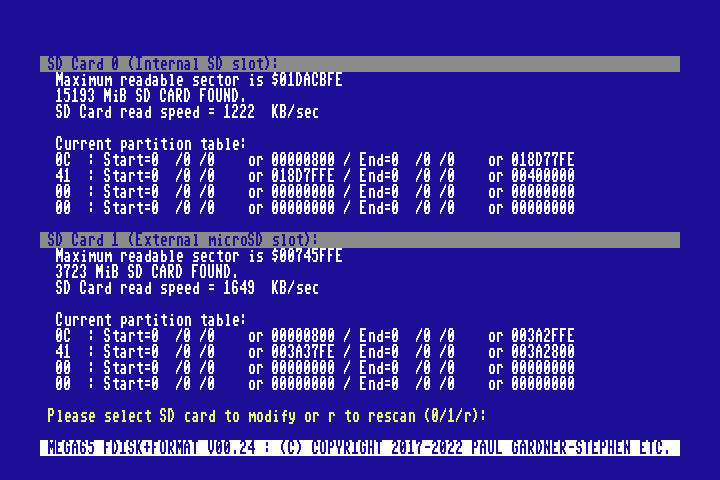
\includegraphics[width=0.7\textwidth]{images/ss-m65fdisk-busselect.png}
\end{center}

Select the card that you want to prepare: \megakey{0} for the internal SD card, \megakey{1} for the external microSD card. If you have two cards installed, {\em be careful to choose the correct card slot.}

The SD Card Utility prompts for confirmation to erase the SD card. As one last precaution, you must type the phrase {\tt DELETE EVERYTHING} in all capital letters, then press \specialkey{RETURN}, to proceed. (If you wish to abort this process, it is safe to switch off the MEGA65 at this time.)

\begin{center}
  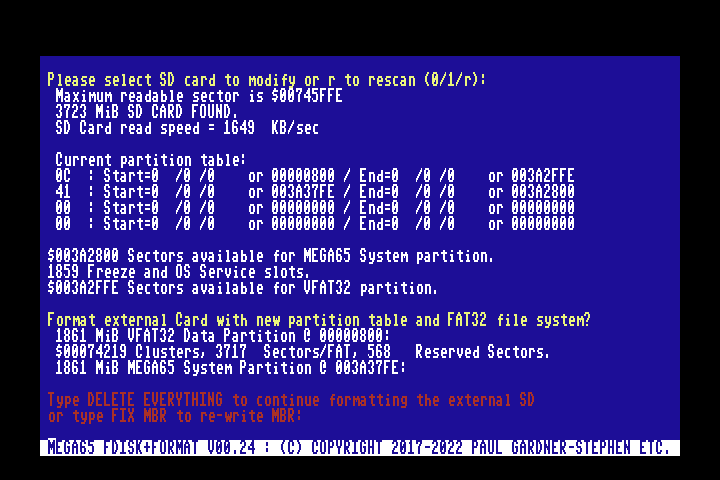
\includegraphics[width=0.7\textwidth]{images/ss-m65fdisk-typesomething.png}
\end{center}

The utility erases the SD card and sets up the partitions. When it is finished, it prompts to install the system files. The system files (with filenames ending in {\tt .M65} and {\tt .ROM}) are embedded in the core, and are copied to the FAT32 partition for use. If you have installed an updated MEGA65 core in slot 1, select it, otherwise select the factory-installed MEGA65 core in slot 0. (If you just received your MEGA65, slot 0 is the only option.)

\begin{center}
  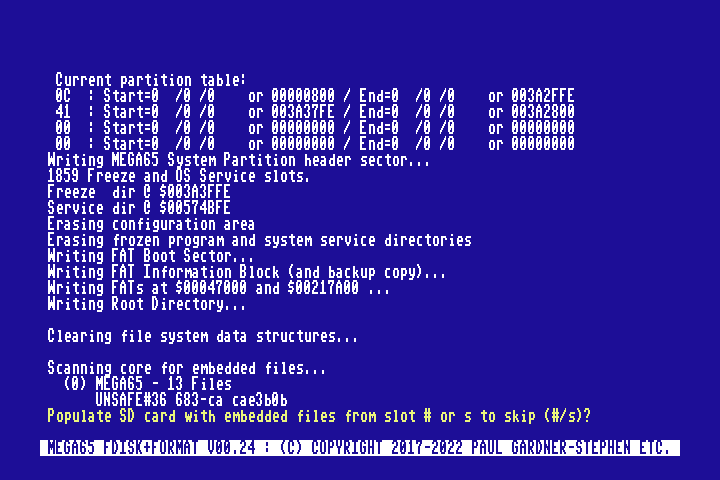
\includegraphics[width=0.7\textwidth]{images/ss-m65fdisk-populate.png}
\end{center}

When prompted, reboot the machine.\footnote{If you select a core that does not have {\tt MEGA65.ROM} as one of the embedded files, the utility will prompt you to move the SD card to your PC to copy this file onto it. This only happens when using a MEGA65 core from somewhere other than an official MEGA65 release package. For more information about cores and obtaining {\tt MEGA65.ROM}, see chapter \vref{cha:cores}.}

\subsection{Obtaining the Bundled Software}

The system files copied to the freshly formatted SD card do not include the bundled software that was included with the original SD card in the internal card slot. You can use your PC to copy these files off of the original SD card, then copy them back onto the new SD card.

The MEGA65 Filehost website\index{Filehost website} hosts all manner of files you can download for your MEGA65. This includes the latest versions of the platform components, alternate cores, and hundreds of games, demos, and applications produced by the MEGA65 community. This also includes the bundled software from the original SD card included with the computer.

If you no longer have the bundled software files, you can obtain them from the MEGA65 Filehost website. Visit the following URL, then search for ``MEGA65 Release SD Card - Intro Disk Extras.''

\url{https://files.mega65.org}

\chapter{Upgrading the MEGA65}

\section{How a MEGA65 Can Be Upgraded}
\label{cha:cores}

The MEGA65 platform consists of three major components:

\begin{enumerate}
  \item The {\bf MEGA65 core},\index{Core} a description of the chipset to run on the FPGA
  \item The {\bf ROM},\index{ROM} code that defines the Commodore-style operating system (KERNAL) and BASIC
  \item {\bf System software} for features such as the Freezer menu\index{Freezer menu}
\end{enumerate}

You can upgrade these components as new releases are published. You can also replace one or more of these components individually. In the case of the core and ROM, you can even have multiple versions installed simultaneously and switch between them. For example, instead of the latest MEGA65 ROM, you can switch to the original Commodore 65 prototype ROM. Or, you could switch to another core that causes your MEGA65 hardware to behave like a different computer entirely, such as a Commodore 64 or a ZX Spectrum.

The ROM and system software are files that reside on the SD card, and upgrading them is as simple as replacing the files. To upgrade the core, you use a process to install a core file into the MEGA65's core flash memory. This chapter describes this process.

\subsection{What is a Core?}
\index{Core!definition}

The MEGA65 hardware architecture is based on a versatile chip called a ``Field Programmable Gate Array,'' or FPGA.\index{Field Programmable Gate Array (FPGA)} This is a special kind of computer chip that can be programmed to impersonate other chips. It does this by configuring a giant array of logic gates to reproduce circuits. FPGAs are not an emulation, but an electronic re-creation of other chips. FPGA code is sometimes referred to as {\em firmware,} a term you may recognize from modern computers and other devices.

Your MEGA65 was programmed at the factory to re-create a chipset based on the original Commodore 65, designed by the MEGA65 team. You can re-program the MEGA65 FPGA to upgrade to new versions of the MEGA65 chipset, or to replace the chipset with that of an entirely different computer!

Each possible chipset is known as a {\em core}. The MEGA65 can store up to eight cores, and you can switch between these cores by accessing a menu when you switch on the computer. You can also use this menu to load a new core from a file on the SD card, a process known as {\em flashing}.

Members of the MEGA65 community have made several useful and fun alternate cores for the FPGA hardware. \href{https://github.com/MJoergen/C64MEGA65}{{\em C64 for MEGA65}} by MJoergen and sy2002 re-creates the original Commodore 64 computer with a high degree of accuracy, perfect for running Commodore 64 games, demos, and applications. Other cores re-create the ZX Spectrum, the Game Boy, and even the original Galaga arcade machine hardware. The MEGA65's FPGA is powerful enough to re-create nearly all 8-bit home computers, and likely some 16-bit computers and consoles such as the Commodore Amiga. The MEGA65 hardware design, board layout, FPGA core, and other information are all available for free under various open-source licenses, so anyone is free to create other cores for the MEGA65 hardware.

\section{Determining the Versions of Things}
\label{sec:versions}

All components of the MEGA65 platform have a version identifier. The MEGA65 can display the version identifiers for all of its components using the MEGA65 Information utility.\index{MEGA65 Information Utility}

To open the MEGA65 Information utility:

\begin{enumerate}
  \item Switch on the MEGA65, and allow it to boot to BASIC.
  \item Open the Freezer:\index{Freezer menu} press and hold \widekey{RESTORE} for one second then release it.
  \item Press \specialkey{HELP}. The MEGA65 Information utility will open.
\end{enumerate}

\begin{center}
  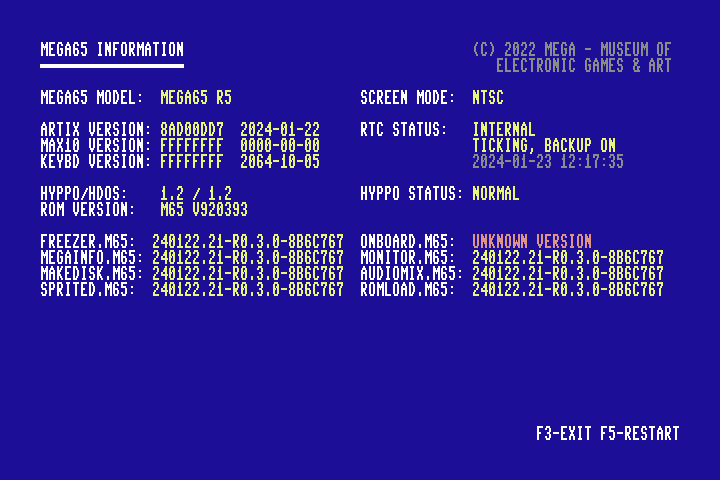
\includegraphics[width=0.7\linewidth]{images/megainfo.png}
\end{center}

Take note of these version identifiers:
\nopagebreak
\begin{center}
\setlength{\tabcolsep}{1mm}
\begin{tabularx}{\textwidth}{|X|p{7cm}|}
  \hline
  {\bf Label and Example} & {\bf Description} \\
  \hline
  MEGA65 Model\newline {\tt MEGA65 R6} & The revision of the hardware. You need to know this when downloading new core files. \\
  \hline
  Artix Version\index{Core!Version}\newline {\tt 8AD00DD7 2024-01-22} & The currently running MEGA65 core. This is a string of eight letters and numbers, and also a build date. \\
  \hline
  ROM Version\index{ROM!Version}\newline {\tt M65 V920393} & The currently running ROM. For MEGA65 ROMs, this is a sequential number, with larger numbers representing newer releases. \\
  \hline
  System files (.M65)\newline {\tt 240122.21-R0.3.0-8B6C767} & Each of the system software files has its own version identifier. Typically, you do not need to know these: you will upgrade these along with each core. The identifier is similar to the core version, but does not always match the currently running core. \\
  \hline
\end{tabularx}
\end{center}

Press \specialkey{F3} to exit to the Freezer, then \specialkey{F3} again to exit to BASIC.

Each core has a separate version for each hardware revision. As of the year 2024, the production models of the MEGA65 have used two different main board revisions, known as ``R3'' (more specifically ``R3A'') and ``R6.''\footnote{The MEGA65 ``DevKit'' model sold in the year 2020 is revision ``R3.'' It is also possible to run the MEGA65 core on certain FPGA development boards, with a separate version of the core file for each.}\index{Hardware revisions}

The MEGA65 core is available for all hardware revisions. If you are installing an alternate core and it is not available for your hardware revision, contact the author of the core.

\section{Obtaining the Latest Files}

You can download the latest MEGA65 core, ROM, and system software from the MEGA65 Filehost website.\index{Filehost website} Due to distribution restrictions for the Commodore 65 ROM code, some files require a Filehost account registered to a MEGA65 owner to access. All owners of the MEGA65 have a license to all versions of this ROM code.\footnote{There is a procedure for non-owners to get the latest MEGA65 ROM, such as to use with the \href{https://github.lgb.hu/xemu/}{Xemu MEGA65 emulator}. This involves downloading \href{https://www.c64forever.com/}{C64 Forever Free Express Edition} from Cloanto, extracting the original Commodore 65 prototype ROM file, then using a tool to apply a patch that you can download from Filehost. The full process is described in the following article: \url{https://mega65.org/rom-faq}}

Visit the following URL in your web browser:

\url{https://files.mega65.org}

\begin{center}
  \fbox{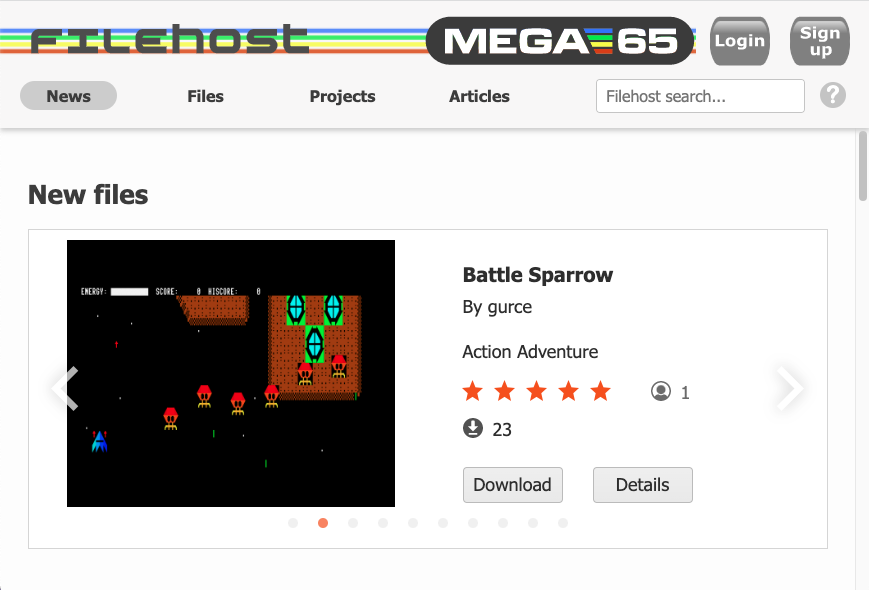
\includegraphics[width=0.7\linewidth]{images/filehost_notsignedin.png}}
\end{center}

To register a Filehost account with your owner code:

\begin{enumerate}
  \item Visit \href{https://files.mega65.org}{the Filehost website}. Click ``Sign Up.'' Follow the prompts to create an account.
  \item Locate your owner code.\index{Owner Code} This is a code printed on a piece of paper that was included with your MEGA65 (possibly inserted into this manual). It looks something like this: {\tt 123-ABC-456}
  \item Click the user icon in the upper-right corner of the Filehost screen. In the pop-up menu, select ``Redeem Code.'' Enter your owner code as prompted.
\end{enumerate}

\begin{center}
  \fbox{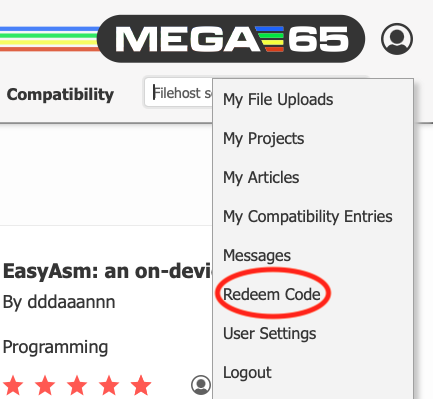
\includegraphics[width=0.4\linewidth]{images/filehost_redeemmenu.png}}
\end{center}

To download the latest release package:

\begin{enumerate}
  \item Click the ``Files'' tab of the Filehost website.
  \item In the search box on the left-hand side, type: ``release'' The list will update to show only files with that word in the title.
  \item Locate the entry named, ``MEGA65 Core Release Package (mega65r6) incl. ROM,'' where ``mega65r6'' matches your hardware revision. (To confirm your hardware revision, open the Freezer menu, then press \specialkey{Help}.)
  \item Click the entry. Confirm that this release package is for your hardware revision, then click ``Download'' to download the file.
\end{enumerate}

\underline{NOTE}: There is an entry for the Release Package that does not include the ROM that is visible to everyone. To ensure you are using a compatible set of files, get the package that says ``incl. ROM.'' If you don't see an entry that says ``incl. ROM,'' check that you are signed in and that you have redeemed a valid owner code.

\begin{center}
  \fbox{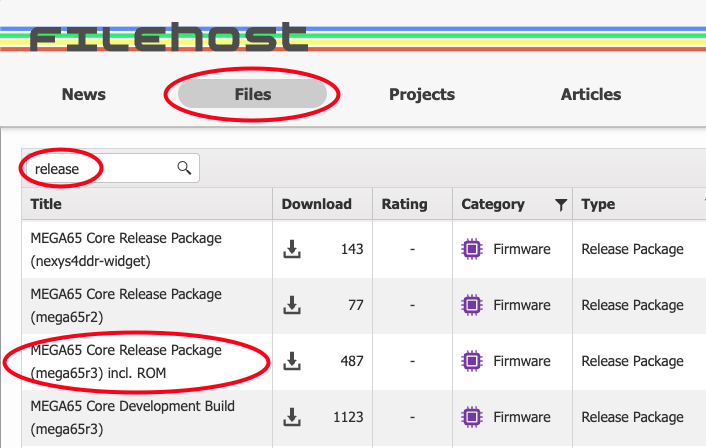
\includegraphics[width=0.7\linewidth]{images/filehost_release.png}}
\end{center}

Extract the downloaded {\tt .7z} archive. You should see a file whose name ends in {\tt .cor}, and a folder of {\tt sdcard-files} that includes one named {\tt MEGA65.ROM}.

\section{The Core Selection Menu}
\index{Core!Core Selection Menu}

The MEGA65 decides which core to load into the FPGA when it starts up. You can interrupt this process to select which core to load.\footnote{Technically, the MEGA65 starts the core in slot 0 to power the core selection menu. After you have made a selection or it chooses a default, it loads the selected core into the FPGA and continues the boot process.}

To open the core selection menu, switch off the computer, then hold the \specialkey{NO\\SCROLL} key and switch on the computer. The core selection menu appears, with the eight core slots numbered 0 through 7.

\begin{center}
  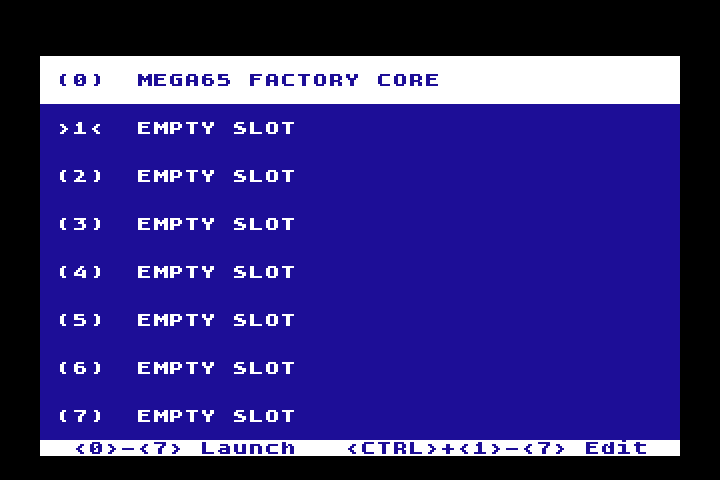
\includegraphics[width=0.7\linewidth]{images/ss-flashmenu.png}
\end{center}

You can select a core to boot using the cursor keys and \specialkey{RETURN}, or you can simply press the number key that corresponds to the slot. The boot process continues with the new core. The MEGA65 will keep running the new core until you switch it off. (Pressing the reset button will not reset which core is being run.)

When you switch on the computer without opening the core selection menu, the MEGA65 looks for a default core. It first checks to see if any core is flagged as the default core (a setting you can change). If none are flagged, then it checks to see if there is a core in slot 1.\footnote{If DIP switch \#4 is in the ``on'' position, the MEGA65 checks slot 2 instead of slot 1. DIP switches are located inside the case, on the main board.} If the slot is empty, it uses slot 0.

Your computer comes with the MEGA65 core in slot 0 installed at the factory. It is recommended that you do not upgrade the factory-installed core unless advised to do so by the MEGA65 team. Instead, install new versions of the MEGA65 core in slot 1.

\section{Upgrading the MEGA65 Core, ROM, and System Files}
\index{Core!Upgrading}\index{ROM!Upgrading}

You can upgrade a core, or install a new core, from the core selection menu. This process reads the {\tt .cor} file from the SD card.

To upgrade the MEGA65 core, ROM, and system files:

\begin{enumerate}
  \item Remove the SD card (or microSD card) from the MEGA65, and connect it to your PC using an SD card reader.\footnote{As an alternative to moving the SD card to your PC, you can transfer files using an Ethernet connection. See chapter \vref{cha:transferring-files}.}
  \item Copy the {\tt .cor} file that you extracted from the {\tt .7z} archive to the SD card.
  \item On your PC, open the {\tt sdcard-files} folder from the {\tt .7z} archive, then copy those files to the SD card, replacing the existing files. Put them in the root of the SD card's file system, not a sub-folder.
  \item Eject the SD card from your PC's operating system, then move it back to the MEGA65.
  \item Open the core selection menu: switch off the MEGA65, then hold \specialkey{NO\\SCROLL} while switching it back on.
  \item Hold \specialkey{CTRL} then press the number of the slot you want to upgrade. The slot editor opens.
  \item Press \specialkey{F3} to load a core file. The file selector opens. Use the cursor keys to select the {\tt .cor} file, then press \specialkey{RETURN}.
  \item Press \specialkey{F8} to flash the core slot. Allow the flashing process to complete. This takes several minutes.
  \item When the flashing process is complete, press any key to return to the core selection menu.
\end{enumerate}

The slot editor looks like this:

\begin{center}
  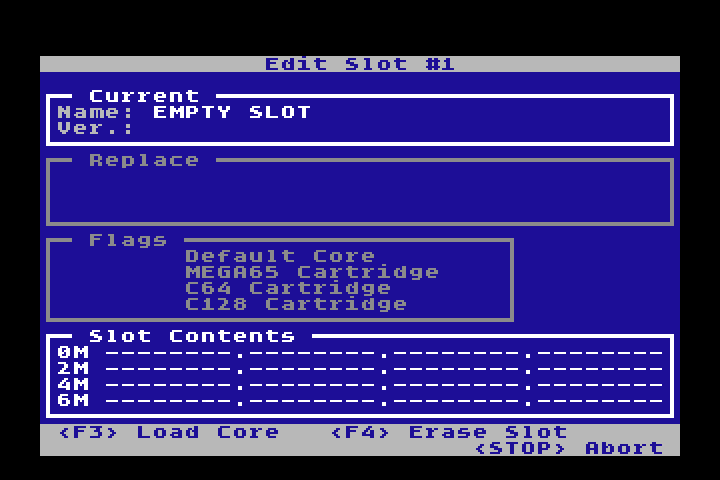
\includegraphics[width=0.7\linewidth]{images/ss-flashmenu-sloteditor.png}
\end{center}

When you load a core file, it prompts you to select the {\tt .cor} file on a screen that looks similar to this:

\begin{center}
  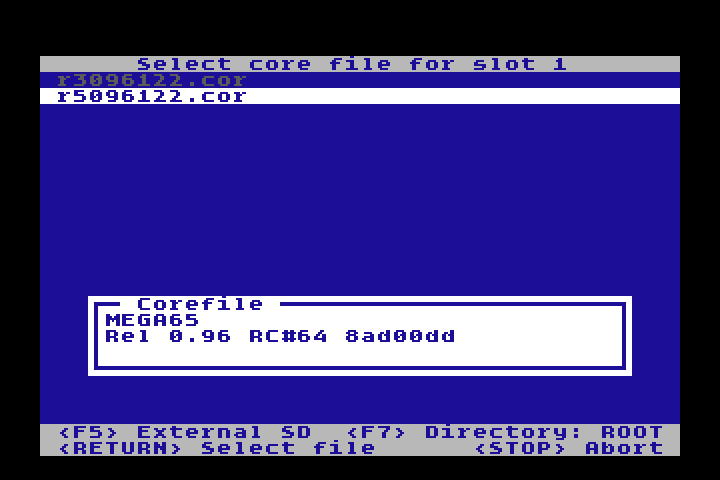
\includegraphics[width=0.7\linewidth]{images/ss-flashmenu-selectcore.png}
\end{center}

Once you have selected the core, the slot editor shows the change it intends to make to the slot. After you start the flashing process, the display shows the progress.

\underline{NOTE}: Do {\em not} switch off your computer or disconnect power until after this step is complete.

\begin{center}
  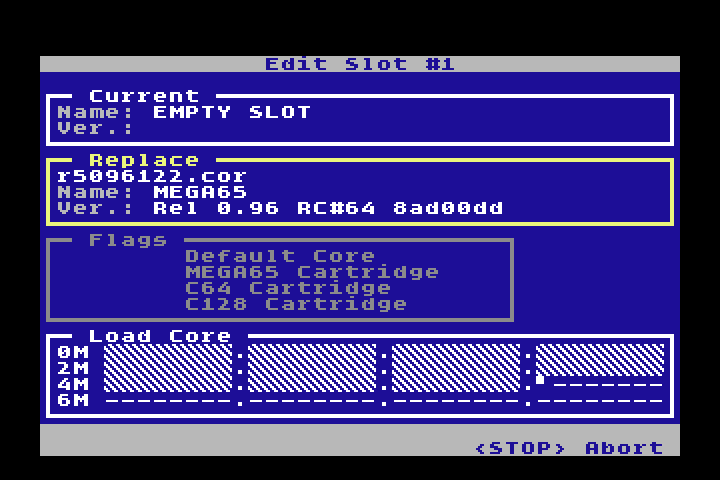
\includegraphics[width=0.7\linewidth]{images/ss-flashmenu-loading.png}
\end{center}

When the message "Core was successfully flashed" is displayed, the process is complete.

\begin{center}
  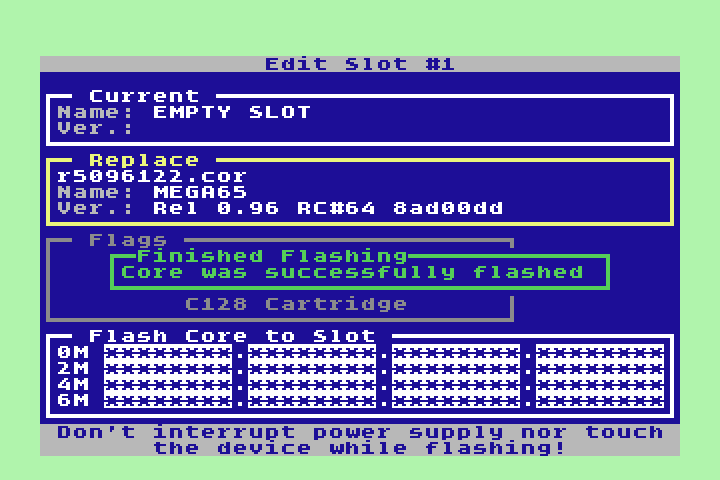
\includegraphics[width=0.7\linewidth]{images/ss-flashmenu-complete.png}
\end{center}

It is now safe to switch off your computer. Press any key to return to the core selection menu, or switch the computer off then on again to start the default core.


\section{Installing Alternate Cores and ROMs}

Installing an alternate core, such as the C64 core,\index{Core!C64 core} uses the same steps for flashing the core to a slot.

It is recommended to use slots 2 through 7 for alternate cores, and reserve slot 1 for the latest MEGA65 core. Of course, there is nothing stopping you from installing an alternate core in slot 1, so that the MEGA65 behaves as a different type of computer when you switch it on. You can always choose the MEGA65 core from the core selection menu.

You can keep more than one version of the MEGA65 ROM on the SD card. When booting the MEGA65 core, you can select one of these ROMs by holding down a number key during boot.

To install alternate ROMs, copy them to the root of the SD card with a filename such as {\tt MEGA65x.ROM}, where {\tt x} is a number between 1 and 7. To boot the alternate ROM, hold the corresponding number key down while the MEGA65 core starts. If you do not hold down a number, it boots to {\tt MEGA65.ROM} by default.

There are several reasons you might want to keep alternate ROMs on your SD card:

\begin{itemize}
  \item You are helping to test a new beta release of the ROM, and do not wish to make the beta version your default ROM.
  \item You want to try the original Commodore 65 prototype ROM. The MEGA65 core maintains backwards compatibility with the C65 ROM that was in progress by Commodore before they cancelled the project. It is buggy and incomplete, but is still an interesting historical artifact.
  \item You want to try an alternate ROM developed by the MEGA65 community. One such ROM is the MEGA65 OpenROM, a project to create an all-new ROM released under an Open Source license without any original Commodore material.
\end{itemize}

Several alternate ROMs came with your MEGA65 SD card, installed at the factory. Try rebooting your computer while holding down a number key to see what happens!

\section{Setting Core Flags}

There are several options ("flags") that you can select for a core in the core editor.

To change flags for a core, edit the core slot. Press the number key that corresponds to the flag to toggle its value. Save the flags to the slot by flashing the result: press \specialkey{F8}. You can either set flags before flashing new core data, or you can flash just the new flag settings without replacing the core data.

To set a core to be the default core used when the MEGA65 is switched on without \specialkey{NO\\SCROLL} held down, set the "Default core" flag. If no core is set as the default core, then slot 1 is used as the default (or slot 2 if DIP switch \#4 is set to on).

The "cartridge" flags determine which core is selected when a cartridge is present in the expansion slot. This allows you to choose a different default core based on the type of the cartridge. For example, you can set the MEGA65 core to handle MEGA65 cartridges, and a different core to handle C64 cartridges. By default, the MEGA65 core will handle C64 cartridges using "GO64" mode. You may prefer to change this to use the C64 core that you install separately.

\begin{center}
  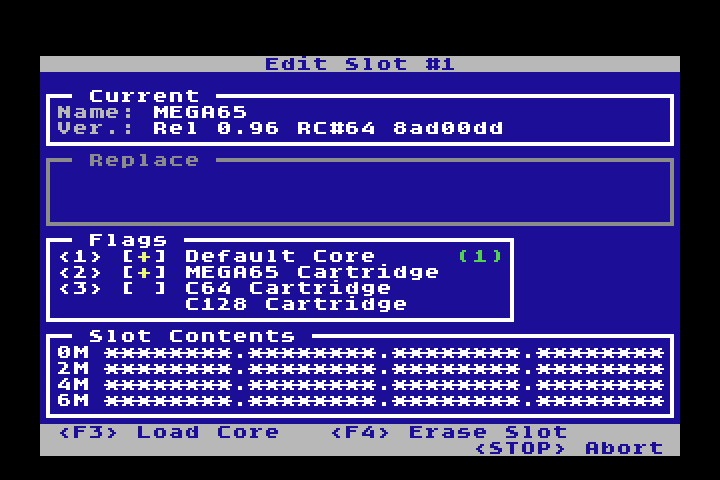
\includegraphics[width=0.7\linewidth]{images/ss-flashmenu-flags.png}
\end{center}

\section{Erasing a Core Slot}

The flashing process replaces whatever is in a core slot with the new core. If a core is already installed in the slot, flashing overwrites the existing core.

If you wish to delete a core and leave the slot empty, edit the slot, press \specialkey{F4} to set the replacement to "Erase slot," then press \specialkey{F8} to flash the slot with empty data.

\section{Upgrading the Factory Core in Slot 0}
\index{Core!Upgrading Slot 0}

It is possible to upgrade the factory-installed MEGA65 core in slot 0. You only need to do this in rare cases, such as if a newer version of the MEGA65 core includes changes or bug fixes for the start-up process. It is recommended that you do not upgrade slot 0 unless the announcement for the release suggests that you do so. Most MEGA65 core upgrades are fully functional in slot 1, without needing to upgrade slot 0.

It is important that at least one core slot contains a functioning MEGA65 core. If something goes wrong during the flashing process, this may result in a non-functioning core in that slot. To help prevent accidents, the procedure for flashing slot 0 is slightly different from that of the other slots, and only an official MEGA65 core can be flashed to slot 0.

{\em Please read these instructions carefully before starting the procedure.} To upgrade the core in slot 0:

\begin{enumerate}
  \item Install the latest MEGA65 core in slot 1, using the procedure described earlier. The core must be in the default non-zero slot to recover from any problems when updating slot 0.
  \item Launch core slot 1 to confirm that it works.
  \item Return to the core selection menu: switch off the MEGA65, then hold \specialkey{NO\\SCROLL} while switching it back on.
  \item Hold the \megasymbolkey and press the comma key to open the editor for slot 0.
  \item Read the information screen, then type the word {\tt CONFIRM} using uppercase letters and press \specialkey{RETURN}.
  \item Repeat the remainder of the flashing procedure to select the core file and flash the slot.
\end{enumerate}

\underline{NOTE}: If you have a revision R3A MEGA65 and have not previously upgraded slot 0, the \megasymbolkey and the comma key will not start the procedure: you have an older slot 0 core that does not have this feature. You can work around this by restarting the core selection menu with slot 1. From the core selection menu, prepare to hold down \specialkey{NO\\SCROLL}, press the \megakey{1} key to boot into the core then immediately press and hold \specialkey{NO\\SCROLL}. The core selection menu re-opens using slot 1. Press \megasymbolkey and the comma key to complete the slot 0 upgrade.

If something goes wrong during the slot 0 flashing process, your MEGA65 may not start correctly. Before doing anything else, switch on your MEGA65, and wait a minute or so. After a while, it should notice that there is no valid core in slot 0, then proceed to start the core in slot 1. You can hold \specialkey{NO\\SCROLL} during this to open slot 1's core selection menu and restart the flashing process.

If the MEGA65 cannot boot any core after several minutes, it may be stuck. You may be able to recover using a device known as a ``JTAG interface'' that connects your PC to the MEGA65 main board. This allows you to inject a bitstream directly into the FPGA. The part is inexpensive but not always available. Contact the MEGA65 team on the Discord (\url{https://mega65.org/chat}) for assistance.

Core slot 0 cannot be assigned flags, such as to be the default core or to be associated with cartridge types. Slot 0 will be used for these purposes if no other core is installed. It is recommended that you keep the latest MEGA65 core in slot 1, in addition to flashing slot 0.


\section{Understanding The Core Booting Process}
\nopagebreak
This section summarises how the MEGA65 selects which core to start with when it is switched on. The process is shown in the following figure:
\nopagebreak
\includegraphics[width=\linewidth]{images/illustrations/flashmenu-flowchart.pdf}

The booting process is governed by two facilities:
\begin{itemize}
  \item The Hypervisor (also known as HYPPO), which operates at a level above the KERNAL. One of its responsibilities is to manage aspects of the boot process. For more details on the Hypervisor, refer to
\ifdefined\printmanual
the {\bf MEGA65 Book}.
\else
 \bookvref{sec:hypervisor-mode}.
\fi
    In the diagram, activities performed by the Hypervisor have been highlighted in green.
  \item The Core Selection Menu program (also known as ``MegaFlash''), which provides a list of available core slots to choose from. In the diagram, activities performed by MegaFlash have been highlighted in blue.
\end{itemize}

When the MEGA65 is switched on, it does the following:
\begin{itemize}
\item Loads the bitstream stored in slot 0 of flash memory. If that is the MEGA65 Factory Core, the MEGA65
  HYPPO Hypervisor starts.
\item If it is the first boot since power-on (which implies that you are running from slot 0), HYPPO starts the Flash Menu program (aka MegaFlash) -- but note that the Flash Menu in
      this mode may not show anything on the screen to indicate that it is running!
\item The Flash Menu then checks if \specialkey{NO\\SCROLL} is being held down.
\item If it is, the Flash Menu program shows its display, allowing you to select or re-flash a core.
\item If \specialkey{NO\\SCROLL} is {\em not} being held down, the Flash Menu program checks if Flash Slot 1 contains a valid
      core.
\item If it does, then the Flash Menu program attempts to load that core.
\item If it succeeds, then the system reconfigures itself for that core, after which the behaviour of the system is
      according to that core.
\item If it fails, the keyboard will go into ``ambulance mode'', showing flashing blue lights to indicate that some
      first-aid is required. Note that in ambulance mode the reset button has no effect: You must switch the
      MEGA65 off and on again.
\end{itemize}

If you have selected a different core in the Core Selection Menu, the process is similar, except that the ambulance lights will appear for only a limited time, as the FPGA will automatically search through the flash memory until it finds a valid core. If it gets to the end of the flash memory, it will start the MEGA65 Factory Core from slot 0 again.

\chapter{Using Disks and Disk Images}

\section{Disk Drives}
\label{cha:using-disks}
\index{Disk Drives}

The MEGA65 has a built-in 3.5" floppy disk drive, and supports Commodore-style external disk drives via the IEC serial port on the back of the computer. The IEC port also supports other external IEC storage devices, such as the SD2IEC.\index{SD2IEC device} Some IEC storage devices can be connected in a chain and used at the same time.

The MEGA65 also includes a ``virtual'' disk drive that can mount D81 or D64 disk image files\index{D81 disk image}\index{D64 disk image} stored on the SD card. Most MEGA65 software that you download from the Internet is in the form of a D81 disk image. Programs for the Commodore 64 are often distributed in the form of a D64 disk image. You can create a new D81 disk image directly from the MEGA65, and start saving your BASIC programs to the SD card without any additional hardware. You can also copy files between physical floppy disks and disk images.

The Intro Disk Menu\index{Intro Disk} that you saw when you first switched on the computer is a program on a D81 disk image, a file named {\tt MEGA65.D81} on the SD card. The MEGA65 is initially configured to boot this disk image automatically. You can change this in the Configuration Utility.\index{Configuration!Utility} (Refer back to chapter \vref{cha:configuringyourmega}.)

You can manage disk drives and virtual disk images from the Freezer menu.\index{Freezer menu} Some of these operations can be performed with BASIC commands such as {\bf MOUNT}.\index{BASIC 65 Commands!MOUNT}

\subsection{Unit Numbers and Drive Numbers}
\index{Disk Drives!Terminology}
\index{Connections!IEC}

Each disk drive (physical or virtual) is accessed via a {\it unit} number.\index{Unit number (IEC devices)} With vintage Commodore computers, the unit number refers to an IEC device connected to the computer. Commodore reserved unit numbers in the range 0 -- 31 for devices of various purposes, with 8 -- 11 reserved for disk drives. If you've ever used a Commodore 64 and typed \screentext{LOAD "*",8,1}, the ``8'' refers to the disk drive connected as unit 8. BASIC 65 disk commands use unit 8 by default, and accept a {\bf U} parameter to change it, such as: \screentext{DLOAD "MYPROGRAM",U9}\index{BASIC 65 Examples!DLOAD}\index{BASIC 65 Examples!LOAD}

With the MEGA65, you can assign a unit number to the virtual disk drive with a disk image mounted, or to the internal 3.5" floppy drive. You must mount a disk image or the internal 3.5" floppy drive to a unit number before it can be used. Any message sent to a unit number assigned to a virtual disk or the internal floppy drive is handled by the MEGA65. All other messages are sent to the IEC serial port.

Disk commands also accept an optional parameter to specify a {\it drive} number.\index{Drive number (IEC devices)} This is only needed when connecting a vintage dual floppy drive via the IEC port, such as the Commodore 4040, 8050, or 8250. Every disk drive assigns drive number 0 to the first drive. Dual-drive units assign a drive number of 1 to the second drive. Dual disk drives are usually equipped with an IEEE-488 interface, and need an IEEE-488 to IEC converter to be used on the MEGA65. BASIC 65 disk commands use drive 0 by default, and accept a {\bf D} parameter to change it.


\section{Using Virtual Disk Images}
\index{Disk Drives!D81 Images}

The MEGA65 provides two ``managed drives'' that supplement drives connected to the IEC port. The first managed drive can be assigned either a D81 or D64 disk image file on the SD card, or it can be assigned to the built-in 3.5" floppy drive. The second managed drive can also be assigned a D81 or D64 disk image file, for up to two virtual disks mounted at the same time.\footnote{Commodore originally intended to release a new external 3.5" floppy drive called the ``1565'' to go with the Commodore 65, connecting to a dedicated non-IEC port. The MEGA65 project has ambitions to someday produce such a drive, and if it does, this would be assigned to the second managed drive.}

The first managed drive can be set to unit 8 or 10, and the second managed drive can be set to unit 9 or 11.

\subsection{Where to Get Disk Image Files}

The MEGA65 Filehost website\index{Filehost website} hosts a library of MEGA65 software produced by the community. You can browse or search for software, download a title, then copy the disk image to the SD card using either your PC or the Ethernet file transfer tool.

\url{https://files.mega65.org/}

\subsection{Mounting Disk Images with the Freezer}

Open the Freezer menu:\index{Freezer menu} hold \widekey{RESTORE} for one second, then release it. Notice the current drive mounting settings in the lower-right of the screen.

\begin{center}
  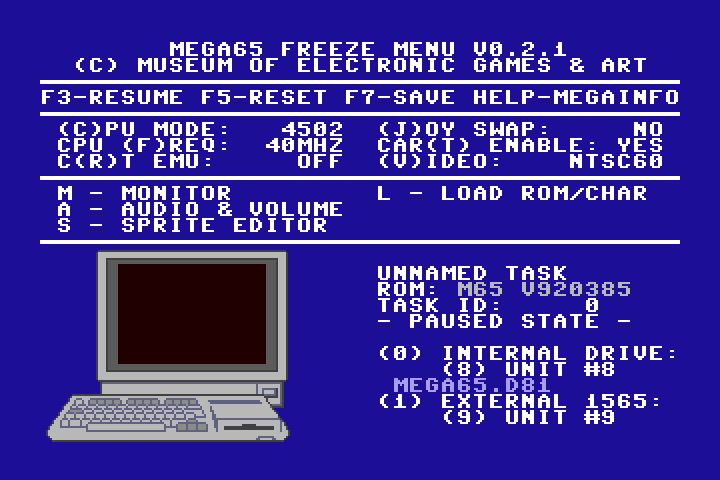
\includegraphics[width=0.7\linewidth]{images/freezer.png}
\end{center}

To mount a disk image on unit 8 or 10, select the first managed drive by pressing \megakey{0}. To mount a disk image on unit 9 or 11, select the second managed drive by pressing \megakey{1}. This opens the SD card file browser.

\begin{center}
  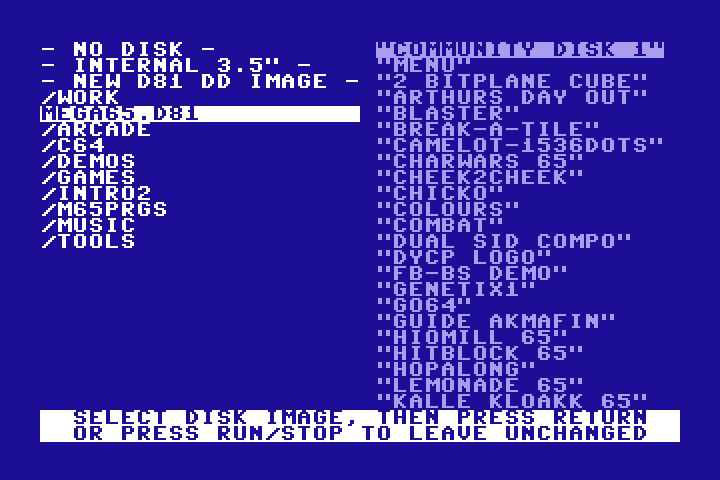
\includegraphics[width=0.7\linewidth]{images/d81-file-browser.png}
\end{center}

Use the cursor keys to select a disk image, then press \widekey{RETURN}. The Freezer screen shows the selected disk image is now associated with the managed drive.

From the main Freezer screen, press \megakey{8} or \megakey{9} to toggle the unit number assigned to the first or second managed drive, respectively.

\subsection{Mounting Disk Images from BASIC}

The BASIC {\bf MOUNT} command\index{BASIC 65 Commands!MOUNT} can mount a disk image from the SD card without having to open the Freezer. This command can be entered at the \screentext{READY} prompt, or be used as part of a program.

To mount a disk image on unit 8, enter {\bf MOUNT} with the full filename in double-quotes, including the {\tt .D81} or {\tt .D64} suffix:

\begin{screencode}
MOUNT "MEGA65.D81"
\end{screencode}

To mount a disk image to unit 9, provide the {\bf U} argument:

\begin{screencode}
MOUNT "MEGA65.D81",U9
\end{screencode}

\subsection{Creating a New Disk Image}
\index{Disk Drives!D81 Images}

You can create a new empty D81 disk image from within the MEGA65 Freezer.\index{Freezer menu}

\begin{enumerate}
\item Open the Freezer.
\item Press \megakey{0} to select the first managed drive.
\item At the top of the file list, select: \screentext{- NEW D81 DD IMAGE -}
\item When prompted, enter a name for the disk. (Omit the {\tt .D81} suffix; this will be added automatically.)
\end{enumerate}

The new disk image is created on the SD card and mounted to the first managed drive. It is formatted and ready to use.

\subsection{Managing SD Card Files in Sub-directories}

Once you have spent some time on Filehost downloading games and applications, you will eventually have a large collection of disk images on your SD card. You may wish to organize these files into sub-directories (folders). You can create these folders with the SD card connected to your PC, or with the Ethernet file transfer tool.

The Freezer supports sub-directories in its file browser. Each sub-directory name begins with a slash (\screentext{/}). Select a folder to list its files. To return to the previous folder, select: \screentext{/..}

The MEGA65 maintains a ``current working directory'' that is used as the base directory for BASIC commands such as {\bf MOUNT}. To change the current working directory from BASIC, use the {\bf CHDIR} command\index{BASIC 65 Commands!CHDIR} with the {\bf U12} argument:\index{BASIC 65 Examples!CHDIR}\index{BASIC 65 Examples!MOUNT}

\begin{screencode}
CHDIR "DEMOS",U12

MOUNT "XANADU.D81"
\end{screencode}

\underline{NOTE}: Support for sub-directories on the SD card is a work in progress. If a disk image in a sub-directory is mounted, it will become un-mounted by any action that changes the current working directory. Some features that use files may not support files in sub-directories. It is not currently possible to create a new disk image in a subdirectory from the Freezer. We hope to improve this in a future update.


\section{Using the Internal 3.5" Floppy Disk Drive}

The MEGA65 has a built-in 3.5" floppy disk drive, similar to what was intended for the Commodore 65. You can use physical floppy disks to store your programs and data. Some MEGA65 software can be purchased on floppy disk.

The internal 3.5" drive must be mounted before it can be used. It can be mounted to unit 8 or unit 10, in the first managed drive.

\subsection{Mounting the 3.5" Drive with the Freezer}

Open the Freezer menu:\index{Freezer menu} hold \widekey{RESTORE} for one second, then release it. Notice the current drive mounting settings in the lower-right of the screen.

Press \megakey{0}, then use the cursor down key to: \screentext{- INTERNAL 3.5" -} Press \widekey{RETURN} to select it. The Freezer menu screen shows that the internal drive is mounted to the first managed disk device.

The \screentext{UNIT \#} for the first device can be either 8 or 10. Press \megakey{8} to toggle between these options. BASIC disk commands default to unit 8, so it is typical to use unit 8 unless you are working with multiple disks at the same time.

The internal 3.5" drive can only be mounted in the first managed drive with unit numbers 8 or 10. It cannot be mounted in the second managed drive (unit numbers 9 or 11).

\subsection{Mounting the 3.5" Drive from BASIC}

You can mount the internal 3.5" disk drive to unit 8 using the BASIC {\bf MOUNT} command. This command works from either the \screentext{READY} prompt or from a program. To mount the internal drive to unit 8, enter the command without arguments:\index{BASIC 65 Examples!MOUNT}

\begin{screencode}
MOUNT
\end{screencode}

The {\bf MOUNT} command can only mount the internal drive to unit 8. You can only mount it to unit 10 from the Freezer menu.

\subsection{DD and HD disks}
\index{Disk Drives!Double-Density (DD) Disks}
\index{Disk Drives!High-Density (HD) Disks}

The MEGA65 disk controller expects a Double Density (DD) floppy disk in the internal 3.5" floppy disk drive.\footnote{It may be possible to support full-capacity HD disks in a future firmware update. The drive hardware is capable of reading HD disks.} Floppy disks are no longer manufactured, and the DD variety can be difficult to find.

You can use a High Density (HD) floppy disk with the drive, with one important modification: you must cover both sides of the hole in the upper-left corner (as seen from the front) of the disk with a small piece of tape. This convinces the drive that the disk is DD, and switches it to a mode compatible with the MEGA65 disk controller. A double-density disk does not have a hole in this location.

\begin{center}
  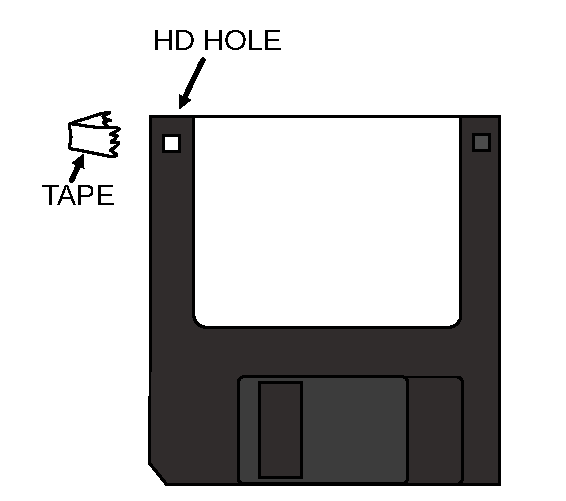
\includegraphics[width=0.75\textwidth]{images/illustrations/floppy_hd.pdf}
\end{center}

\underline{NOTE}: Make sure that the tape covers both sides of the hole.

\subsection{Formatting a Disk}
\index{Disk Drives!Formatting a Disk}

A floppy disk must be formatted before it can be used. The MEGA65's internal 3.5" floppy drive emulates a Commodore 1581 drive, and can use disks formatted in such a drive. You can also format a disk with the MEGA65.

\underline{NOTE}: Formatting a disk erases its contents. Be careful to only do this when you do not need the data on the disk!

To format a physical 3.5" floppy disk using the internal drive:

\begin{enumerate}
\item Open the Freezer.\index{Freezer menu}
\item Mount the internal 3.5" floppy drive to the first managed drive, unit 8.
\item {\it Double-check that unit 8 says:} \screentext{- INTERNAL 3.5" -}
\item Resume the computer: press \megakey{F3}.
\item Insert the floppy disk you wish to format into the internal floppy drive.
\item Enter the BASIC {\bf FORMAT} command, giving it a name ({\tt "MYDISK"}) and a two-character ID ({\tt XX}).\index{BASIC 65 Commands!FORMAT}\index{BASIC 65 Examples!FORMAT}
\begin{screencode}
FORMAT "MYDISK",IXX
\end{screencode}
\item When prompted, enter {\tt YES} and press \widekey{RETURN}.
\end{enumerate}

Formatting the disk takes a minute or so. The drive will make buzzing and clicking noises during the process. Do not switch off the computer or eject the disk until formatting is complete.

You can confirm that the formatting was successful by issuing the {\bf DIR} command.\index{BASIC 65 Commands!DIR} You should see an empty directory listing with the name and ID you specified. Your disk is now ready to use.


\section{Using External IEC Disk Drives}
\index{Connections!IEC}

The MEGA65 works with external disk drives connected to the IEC serial port.

External drives do not need to be mounted. If a unit number is not assigned to the internal 3.5" disk drive or to a disk image, disk operations intended for that unit number will be transmitted to the IEC serial port. It is up to the device connected to the port to recognize its unit number. Some IEC devices have switches that let you set the unit number. Others will only work with a specific number.

If you have an external drive that expects a specific unit number, you will need to make sure the MEGA65 isn't assigning that number to a disk image or the internal drive. Open the Freezer,\index{Freezer menu} then press \megakey{8} or \megakey{9} to toggle the unit number assignments so that they no longer use the needed unit number.\index{Unit number (IEC devices)}

The drive and unit assignments are temporary, and will be reset to their defaults when the MEGA65 is switched off. You will need to re-configure the drive assignments the next time you switch on the computer.


\section{Bootable Disks}
\index{Disk Drives!Bootable Disks}

With older Commodore computers, it was common for software makers to organize the file directory on a floppy disk such that the first file in the list is the main program. The user could then enter the command \screentext{LOAD "*",8,1} to load the main program, and \screentext{RUN} to run it. The asterisk is a wildcard that matches any file, so it matches the first file on the disk, without the user having to type the name of the program.

This method is still common, and the MEGA65 has a quick way to boot such disks: hold \specialkey{SHIFT} and press \specialkey{RUN\\STOP}. This executes the \screentext{RUN "*"} command, which is similar to the familiar command sequence that loads and runs the first program on the disk.\index{BASIC 65 Commands!RUN}

With the C65, Commodore introduced a new way to boot disks. Instead of relying on file order, a disk can have a file named {\tt AUTOBOOT.C65}.\index{AUTOBOOT.C65 file} If this file exists and is a program, the BASIC {\bf BOOT} command will load and run this file.\index{BASIC 65 Commands!BOOT}\index{BASIC 65 Examples!BOOT}

\begin{screencode}
BOOT
\end{screencode}

\subsection{Auto-Booting Disks}

As discussed in chapter \vref{cha:configuringyourmega}, you can use the Configuration Utility\index{Configuration!Utility} to set the MEGA65 to mount either a virtual disk image or the internal 3.5" disk drive automatically during boot.

If the mounted disk is bootable --- that is, it contains a program file named {\tt AUTOBOOT.C65} --- the MEGA65 will load and run the boot program automatically.

This is how the Intro Disk works. The Intro Disk menu is a program named {\tt AUTOBOOT.C65} on the virtual disk image {\tt MEGA65.D81}, which is pre-configured to be the mounted disk on system start-up. When you disable the Intro Disk from its menu, it renames {\tt AUTOBOOT.C65} to {\tt MENU}, such that the disk is no longer considered bootable.

Setting up a boot disk for yourself can be a handy way to configure your computer. You can write a short BASIC program that changes the system font, adjusts the background colour, and sets {\bf KEY} macros to your taste, then save the program as {\tt AUTOBOOT.C65} on a disk that you have configured to mount on system start-up. This program will run every time you switch on your MEGA65.


\section{Accessing the SD Card from BASIC}

Several BASIC 65 commands can operate directly on the MEGA65 SD card as if it were a disk drive. In these cases, the SD card is known as unit 12.

\underline{NOTE}: Unit 12 can only be accessed directly for a few specific operations. It cannot treat the entire SD card as if it were a CBDOS disk.

To list all of the files on the SD card, use the {\bf DIR} command with the \screentext{U12} argument:\index{BASIC 65 Commands!DIR}\index{BASIC 65 Examples!DIR}

\begin{screencode}
DIR U12
\end{screencode}

You can use the optional {\bf P} flag with this command to list the SD card files one page at a time. Press Q to stop at the current page, or any other key to advance to the next page.

\begin{screencode}
DIR U12,P
\end{screencode}

To load or save a PRG file directly from the SD card (that isn't in a disk image), use the \screentext{U12} argument with the {\bf DLOAD} and {\bf DSAVE} commands. You {\em must} include the {\tt .PRG} filename suffix in this case, which is different to using PRG files on disks or disk images.\index{BASIC 65 Commands!DLOAD}\index{BASIC 65 Commands!DSAVE}\index{BASIC 65 Examples!DLOAD}

\begin{screencode}
DLOAD "MYPROGRAM.PRG",U12
\end{screencode}

As shown earlier, the MEGA65 supports sub-directories (sub-folders) on the SD card, and maintains a current working directory for disk operations. To change the current working directory to a subdirectory:\index{BASIC 65 Commands!CHDIR}\index{BASIC 65 Examples!CHDIR}

\begin{screencode}
CHDIR "SUBDIR",U12
\end{screencode}

To change the current working directory to the parent of the current directory:

\begin{screencode}
CHDIR "..",U12
\end{screencode}

The {\bf MOUNT} command can mount a D81 or D64 disk image to a unit number. Even though this command refers to a file on the SD card, it does not use the \screentext{U12} argument. Instead, it uses the {\bf U} argument to set the unit number for the disk being mounted. The {\bf MOUNT} command uses the current working directory set by {\bf CHDIR} to locate the file.


\section{Common Disk Operations}

The following are some examples of common disk operations you can perform at the \screentext{READY} prompt. See the BASIC command reference in appendix \vref{cha:basic-reference} for more information.

Most commands that accept filenames also accept a {\bf U} argument that says which unit has the file. The default unit is 8.\footnote{The default disk unit for BASIC commands is 8 when the computer first starts. You can change it with the {\bf SET DEF} command.\index{BASIC 65 Commands!SET}}

\subsection{DIR}
\index{BASIC 65 Commands!DIR}\index{BASIC 65 Examples!DIR}

To display the directory (list of files) for a disk, use the {\bf DIR} command.

\begin{screencode}
DIR

DIR U9
\end{screencode}

Unlike the Commodore 64 method of loading the disk directory into BASIC memory, the {\bf DIR} command does not modify BASIC memory. It is safe to use {\bf DIR} with a program in memory.

To make larger directories easier to view, {\bf DIR W} (for ``wide'') displays the directory in columns, pausing for each page.

\subsection{DLOAD and RUN}
\index{BASIC 65 Commands!DLOAD}\index{BASIC 65 Examples!DLOAD}
\index{BASIC 65 Commands!RUN}\index{BASIC 65 Examples!RUN}

The {\bf DLOAD} command loads a program from disk into memory. The {\bf RUN} command runs the program currently in memory.

\begin{screencode}
DLOAD "COOLGAME"
RUN
\end{screencode}

You can combine these into one command by providing the filename directly to the {\bf RUN} command.

\begin{screencode}
RUN "COOLGAME"
\end{screencode}

\subsection{DSAVE}
\index{BASIC 65 Commands!DSAVE}\index{BASIC 65 Examples!DSAVE}

The {\bf DSAVE} command saves the BASIC program currently in memory to disk.

\begin{screencode}
DSAVE "MYGAME"
\end{screencode}

By default, this will not overwrite an existing file with the same name. To request that the existing file be overwritten, insert an {\tt @} (at) symbol before the filename, inside the double-quotes.

\begin{screencode}
DSAVE "@MYGAME"
\end{screencode}

Note that save-with-replace is only recommended when using disk images and the 3.5" floppy drive. Older Commodore drives have bugs in this feature that could result in data loss.

\subsection{BACKUP}
\index{BASIC 65 Commands!BACKUP}\index{BASIC 65 Examples!BACKUP}

The {\bf BACKUP} command copies an entire disk from one unit to another. All existing data on the destination disk is erased as part of this process.

\begin{screencode}
BACKUP U8 TO U9
\end{screencode}

You can use {\bf BACKUP} to make disk images from floppy disks, or write disk images to floppy disks, or copy everything from one disk drive to another.

\subsection{COPY}
\index{BASIC 65 Commands!COPY}\index{BASIC 65 Examples!COPY}

The {\bf COPY} command makes a copy of a file. If the source and the destination are different filenames on the same unit, this duplicates the file on the disk.

\begin{screencode}
COPY "MYGAME", U8 TO "MYGAME", U9

COPY "MYGAME" TO "MYGAME-V1"
\end{screencode}

\subsection{RENAME}
\index{BASIC 65 Commands!RENAME}\index{BASIC 65 Examples!RENAME}

The {\bf RENAME} command changes the name of an existing file.

\begin{screencode}
RENAME "MYGAME-V29" TO "MYGAME-FINAL"
\end{screencode}

\subsection{DELETE}
\index{BASIC 65 Commands!DELETE}\index{BASIC 65 Examples!DELETE}

The {\bf DELETE} command deletes a file.

\begin{screencode}
DELETE "JUNKFILE"
\end{screencode}


\subsection{Shortcut Disk Commands}

BASIC 65 provides several shortcuts for common disk commands for use from the \screentext{READY} prompt.

\begin{center}
\begin{tabular}{|l|l|}
\hline
{\bf Shortcut} & {\bf Equivalent Command} \\
\hline
\screentextwide{/} & {\bf LOAD} \\
\hline
$\uparrow$ & {\bf RUN} \\
\hline
$\leftarrow$ & {\bf SAVE} \\
\hline
\screentextwide{@} & {\bf DISK} \\
\hline
\screentextwide{\$} & {\bf DIR} \\
\hline
\end{tabular}
\end{center}

These are intended to be used with a directory listing to launch programs without having to type filenames. For example:

\begin{enumerate}
\item Display the disk's directory listing: type {\bf \$}, press \widekey{RETURN}.
\item Use the cursor keys to move the cursor to the line with the program you want to run.
\item Type {\bf \screentext{$\uparrow$}}, press \widekey{RETURN}.
\end{enumerate}

The selected program loads and runs. Notice that you do not have to clear extra characters from the line. The shortcut knows to ignore everything but the filename in double-quotes, as printed by the directory listing.

\chapter{Transferring Files}

\section{Getting Files to the MEGA65}
\label{cha:transferring-files}
\index{SD Cards!Transferring Files}

While there is plenty of fun to be had writing your own programs for the MEGA65, eventually you will want to run programs written by others. You may also want to back up your MEGA65 programs to your PC for safe keeping.

You can copy D81 virtual disk images to your MEGA65-formatted SD card using any PC, without any special tools or software. Your PC will recognize the data region of the SD card as a FAT32 partition. If you use this method, be aware that some PC operating systems may have unwanted side effects, such as fragmentation of SD card files, or extraneous files created by macOS Finder. These effects are harmless to the data, but may require maintenance to keep the card useful in the MEGA65.\footnote{If the MEGA65 reports a fragmented file, you can use a PC disk defragmentation tool on the data partition. Alternatively, you can copy all files off of the SD card to the PC, re-format the SD card in the MEGA65, then copy the files back from the PC.}

The fastest and most reliable way to transfer files between your PC and your MEGA65 is with an Ethernet cable.\index{Networking!Ethernet} You connect one end of the cable to the RJ45 jack on the rear of the MEGA65. You can connect the other end to your local area network (LAN) router or switch, or connect it directly to your PC. You use software on your PC to initiate file transfers, in either direction: from the PC to the MEGA65, or from the MEGA65 to the PC.

It is also possible to transfer files using a JTAG or UART Serial interface connected to the main board. This is an advanced technique and is not described in this User's Guide. Most people will prefer the Ethernet method.\footnote{JTAG or UART Serial hardware provides access to a debugging interface that may be useful to some programmers. JTAG is also useful for developing FPGA cores. For more information, see the {\it MEGA65 Developer's Guide.}}

\section{Understanding Networking}

The MEGA65 can use Ethernet to connect to or accept connections from other computers on a network. With appropriate software, it can connect to other computers over the Internet.

The MEGA65 Ethernet hardware presents a Media Access Control (MAC) address to the local network.\index{Networking!MAC address} Unlike other Ethernet hardware, the MEGA65's MAC address is not assigned at the factory: it is set in the Configuration Utility. (See chapter \vref{cha:configuringyourmega}.)

To transfer files, you instruct the MEGA65 to make itself available for incoming connections, then use M65Connect (or another tool, such as \texttt{mega65\_ftp}) on your PC to initiate a connection. Your PC's operating system may prompt for permission to grant the tool access to the network when you run it for the first time. The tool uses UDP port 4510 to establish the initial connection with the MEGA65 and assign it a temporary IPv6 address for the file transfer session. This requires a local network router that supports IPv6, which most do.

As an alternative to connecting the MEGA65 to your local network, if your PC has an Ethernet jack, you can connect your MEGA65 directly to your PC with an Ethernet cable. This forms a small local network with no access to the Internet. The procedure for transferring files is the same with a direct connection as with a local network connection.

\section{Obtaining the File Transfer Tools}
\index{M65Connect Application}

{\bf M65Connect} is an application for Windows, Mac, or Linux that facilitates file transfers and other useful features for MEGA65 users. The application has a windowed interface, and also includes command-line tools useful for programming.

To obtain M65Connect:

\begin{enumerate}
\item Visit the MEGA65 Filehost website\index{Filehost website} in a browser: \url{https://files.mega65.org}
\item In the search box in the top right corner, type: ``M65Connect''
\item Select the version of M65Connect for your PC operating system.
\item Click the ``Download'' button.
\item Use your PC to unpack the downloaded archive file.
\end{enumerate}

\subsection{M65Connect for Windows}

The Windows version of M65Connect is in the ``M65Connect'' folder: {\bf M65Connect.exe}. As with most open source software, Microsoft Defender may refuse to run the software, displaying a dialog window. If this happens, click ``More info,'' then click the ``Run anyway'' button that appears.

The command-line tools are in a sub-folder named ``M65Connect Resources,'' such as: {\tt M65Connect Resources\textbackslash{}mega65\_ftp.exe}

\subsection{M65Connect for macOS}

The macOS version of M65Connect is a Mac application bundle: {\bf M65Connect.app}. As with most open source software, macOS does not recognize it as ``signed'' by the developer, and macOS will refuse to run it. To run the application for the first time:

\begin{enumerate}
\item Right-click on the {\bf M65Connect.app} icon. In the pop-up menu, select ``Open.'' A dialog will open.
\item Click the ``Open'' button. The application will open.
\end{enumerate}

On subsequent runs, you can double-click the icon as with any other application.

The command-line tools are inside the application bundle directory, such as: {\tt M65Connect.app/Contents/mega65\_ftp.osx}

\subsection{M65Connect for Linux}

The Linux version of M65Connect is in the ``M65Connect'' folder: {\bf M65Connect}. Double-click it to run.

The command-line tools are in a sub-folder named ``M65Connect Resources,'' such as: {\tt M65Connect Resources/mega65\_ftp}

\section{Enabling Network Listening}
\index{Networking!Network Listening Mode}

By default, the MEGA65 ignores all attempts by other computers to connect to it over the network. Software running on the MEGA65 can listen for network connections, but the MEGA65 does not do this on its own.

To transfer files with M65Connect, you must set the MEGA65 to listen for incoming connection attempts from M65Connect. This requires two steps:

\begin{itemize}
\item Set the DIP switch \#2 on the main board to the ``on'' position.
\item Enable a network listening session by pressing this key combination: \specialkey{SHIFT} + \megakey{\pounds}
\end{itemize}

To set the DIP switch,\index{DIP switches} open the case, as described in \vref{cha:setup}. Locate the DIP switches on the main board, then set DIP switch \#2 to the ``on'' position.

\begin{center}
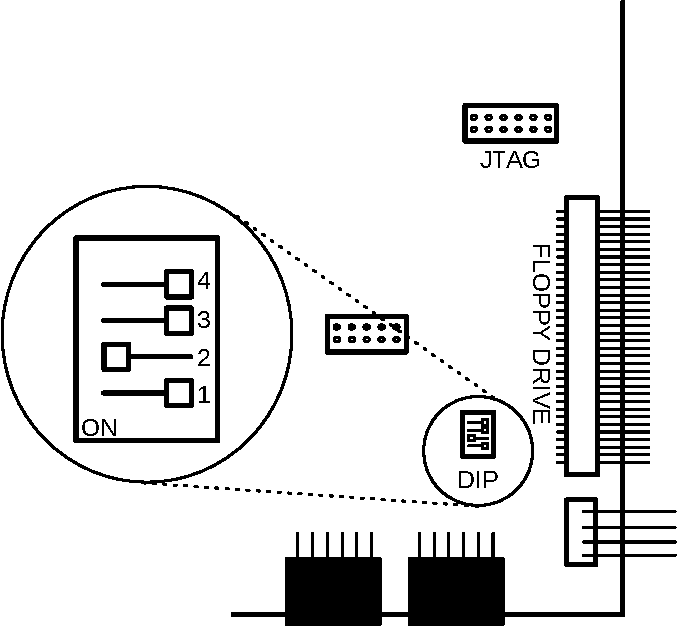
\includegraphics[width=\linewidth]{images/illustrations/mega65-dip2.pdf}
\end{center}

It is safe to leave DIP \#2 in this position for regular operation. It is set to off at the factory to avoid accidental activation.

To enable a network listening session, press \specialkey{SHIFT} + \megakey{\pounds}. The power light blinks between yellow and green when network listening is active.

\begin{center}
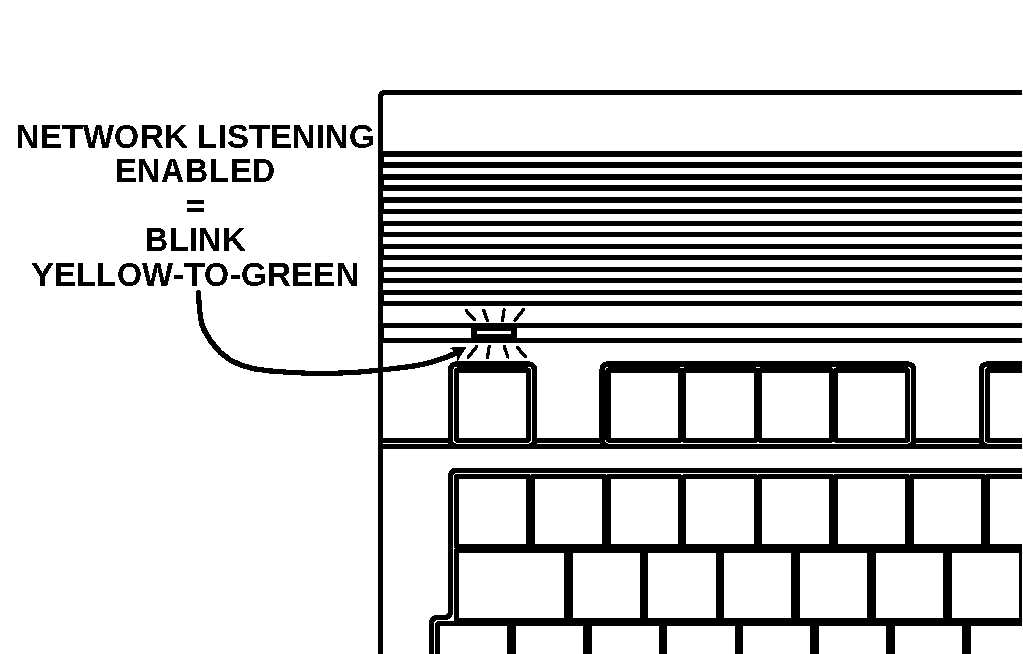
\includegraphics[width=\linewidth]{images/illustrations/mega65-eth-blink.pdf}
\end{center}

\underline{NOTE}: Resetting the computer disables network listening. Press \specialkey{SHIFT} + \megakey{\pounds} to start a new session.

\section{Transferring Files}

To transfer files, you will start a file transfer session using the M65Connect application or the {\tt mega65\_ftp} command-line tool. This connects to the MEGA65 and uploads a file transfer client for use during the session. When you end the session, the MEGA65 resets.

Starting a file transfer session resets the MEGA65. Be sure to save any programs or data before proceeding.

\underline{NOTE}: If you clear memory by resetting the computer, remember to re-enable network listening: press \specialkey{SHIFT} + \megakey{\pounds}, and ensure the power light is blinking.

% \subsection{Transferring Files with M65Connect}
% \index{M65Connect Application}
% TODO: M65Connect instructions are pending an update to M65Connect that implements this procedure.

\subsection{The mega65\_ftp Command-Line Tool}
\index{mega65\_ftp command@\texttt{mega65\_ftp command}}

The {\tt mega65\_ftp} command-line tool initiates a file transfer session with the MEGA65. It can run interactively in the terminal and accept multiple file transfer commands, or it can run non-interactively with those commands provided as arguments.

To start an interactive file transfer session, run the {\tt mega65\_ftp} command, providing the {\tt -e} argument to say you want to use an Ethernet connection.

\begin{verbatim}
% mega65_ftp -e
\end{verbatim}

The tool will upload the file transfer client, and you will see it the client running on the MEGA65. If nothing happens, press Ctrl-C (on the PC) to abort, then double-check that the MEGA65 is connected and that network listening is enabled.

Once connected, the file transfer command prompt looks similar to this:

\begin{verbatim}
MEGA65 SD-Card:/>
\end{verbatim}

To end the session, use the {\tt exit} command. The tool will exit and return to the shell prompt, and the MEGA65 will reset.

\begin{verbatim}
MEGA65 SD-Card:/> exit
%
\end{verbatim}

The following are several useful commands you can use during the file transfer session. Use the {\tt help} command to see a complete list of available commands.

\begin{center}
\begin{tabular}{|l|l|}
\hline
{\bf Command} & {\bf Description} \\
\hline
{\tt put {\it filename}} & Send a file from the PC to the MEGA65. \\
\hline
{\tt get {\it filename}} & Retrieve a file from the MEGA65 to the PC. \\
\hline
{\tt dir} & Display a directory listing of the MEGA65 SD card. \\
\hline
{\tt ldir} & Display a directory listing of the local current working directory. \\
\hline
{\tt mkdir {\it dirname}} & Create a sub-directory on the MEGA65 SD card. \\
\hline
{\tt cd {\it dirname}} & Change the current working directory on the MEGA65 SD card. \\
\hline
{\tt lcd {\it dirname}} & Change the local current working directory. \\
\hline
{\tt help} & Display a list of available commands. \\
\hline
{\tt exit} & End the file transfer session. \\
\hline
\end{tabular}
\end{center}

To invoke {\tt mega65\_ftp} commands without starting an interactive prompt, use the {\tt -c} argument once for each command:

\begin{verbatim}
% mega65_ftp -e -c 'put mydisk.d81' -c 'exit'
\end{verbatim}

The tool will start a session, execute the commands, then terminate. Be sure to issue the {\tt exit} command as the final command to reset the MEGA65, or reset the MEGA65 manually after the file transfer has completed.

%\part{FIRST STEPS IN CODING}
%\chapter{Getting Started in BASIC}
\label{cha:basic-getting-started}

It is possible to code on the MEGA65 in many languages,
however most people start with BASIC.  That makes sense,
because BASIC stands for Beginner's All-purpose Symbolic
Instruction Code: It was made for people like you to get
started with in the world of coding!

A few short words before we dive in: BASIC is a programming
language, and like spoken language it has conventions, grammar
and vocabulary.  Fortunately, it is much quicker and easier
to learn than our complex human languages. But if you pay
attention, you might notice some of these structures, and that
can help you along your path in the world of coding.

If you haven't already read \bookvref{cha:getting-started},
it might be a good idea to do so. This will help you be able to
more confidently interact with the MEGA65 computer.

It's also great to remember that if you really confuse the MEGA65,
you can always get back to the READY. prompt by just pressing the
reset button on the left-hand side of the keyboard, or if that
doesn't help, then by turning it off
and on again using the power switch on the left-hand side of the keyboard.
You don't have to worry about shutting the computer
down properly or any of that nonsense.  The only thing to remember
is that if you had any unsaved work, it will be lost when you switch
the computer off and on again or press the reset button.

Finally, if you don't understand all of the descriptions and information
with an example -- don't worry! We have provided as much information
as we can, so that it is there in case you have questions, encounter problems are
just curious to discover more.  Feel free to skip ahead to the examples
and try things out, and then you can go back and re-read it when you are motivated
to find something out, or help you work though a problem.  And if you don't find
the answer to your problem, send us a message!  There are support forums for the
MEGA65 at \url{https://mega65.net}, and you can
report problems with this guide at:

\url{https://github.com/mega65/mega65-user-guide}

We hope you have as much fun learning to program the MEGA65 as
we have had making it!

\section{Your first BASIC programs}

The MEGA65 was designed to be programmed! When you switch it on,
it takes a couple of seconds to get its house in order, and then
it quickly shows you a ``READY.'' prompt and flashing block called
the cursor.  When the cursor is blinking, it tells you that the
computer is waiting for input.  The ``READY.'' message tells you
that the BASIC programming language is running and ready for you to
start programming.  You don't even need to load any programs --
you can just get started.

\needspace{4cm} % Dont allow following paragraph to separate from
                % following element
Try typing the following into the computer and see what happens:

\begin{screencode}
HELLO COMPUTER
\end{screencode}

\needspace{4cm} % Dont allow following paragraph to separate from
                % following screenshot

To do this, just type the letters as you see them above.  The computer
will already be in uppercase mode, so you don't need to hold \specialkey{SHIFT}
or \specialkey{CAPS\\LOCK} down.  When you have typed "HELLO COMPUTER", press
  \specialkey{RETURN}.  This tells the computer you want it to accept the
  line of input you have typed.  When you do this, you should see a message something
  like the following:

\screenshotwrap{images/getting-started/syntax-error.png}

  If you saw a \screentextwide{SYNTAX ERROR} message something like that one, then congratulations:
  You have succeeded in communicating with the computer!\index{Errors!Syntax}\index{SYNTAX ERROR}
  Error messages sound much nastier than they are.  The MEGA65 uses them, especially
  the syntax error to tell you when it is having trouble understanding what you have
  typed, or what you have put in a program.  They are nothing to be afraid of, and
  experienced programmers get them all the time.

  In this case, the computer was confused because it doesn't understand the word
  ``hello'' or the word ``computer''.  That is, it didn't know what you wanted it to
  do.  In this regard, computers are quite stupid. They know only a few words, and
  aren't particularly imaginative about how they interpret them.

\needspace{4cm} % Dont allow following paragraph to separate from
                % following screenshot

So let's try that again in a way that the computer will understand.  Try typing
  the following in.  You can just type it right away. It doesn't matter that the
  syntax error message can still be seen on the screen.  The computer has already
  forgotten about that by the time it told you \screentextwide{READY.} again.

\begin{screencode}
PRINT "HELLO COMPUTER"
\end{screencode}

Again, make sure you don't use shift or shift-lock while typing it in.  The symbols around
the words \screentextwide{HELLO COMPUTER} are double-quotes.  If you are used to an Australian or American
keyboard, you might discover that they double-quote key is in a rather different place to
where you are used to:  Double-quotes can be typed on the MEGA65 by holding down
\specialkey{SHIFT}, and then pressing \megakey{2}.  Don't forget to press \specialkey{RETURN}
when you are done, so that the computer knows you want it to do something with your input.

If you make a mistake while typing, you can use \specialkey{INST\\DEL} to rub out the mistake
and fix it up.  You can also use the cursor keys to move back and forth on the line while
you edit the line you are typing, but there is a bit of a trick if you have already typed
a double-quote: If you try to use the cursor keys, it will print a funny reversed symbol
instead of moving the cursor.  This is because the computer thinks you want to record
moving the cursor in the text itself, which can be really useful and fun, and which you can
read more about in \bookvref{cha:getting-started}. But for now, if you
make a mistake just press \specialkey{RETURN} and type the messed up line again.

\needspace{4cm} % Dont allow following paragraph to separate from
                % following screenshot
Hopefully now you will see something like the following:

\screenshotwrap{images/getting-started/print-hello-computer.png}

  This time no new \screentextwide{SYNTAX ERROR} message should appear. But if some kind
  of error message has appeared, just try typing in the command again, after
  taking a close look to work out where the mistake might be.

  Instead of an error, we should see \screentextwide{HELLO COMPUTER} repeated underneath
  the line you typed in.  The reason this happened is that the computer
  does understand the word \screentextwide{PRINT}.  It knows that whatever comes after
  the word \screentextwide{PRINT} should be printed to the screen.  We had to put \screentextwide{HELLO
  COMPUTER} inside double-quotes to tell the computer that we want it to be
  printed literally.

  If we hadn't put the double-quotes in, the computer would have thought
  that \screentextwide{HELLO COMPUTER} was the name of a stored piece of information.
  But because we haven't stored any piece of information in such a place,
  the computer will have zero there, so the computer will print the number
  zero. If the computer prints zero or some other number when
  you expected a message of some sort, this can be the reason.

\needspace{4cm} % Dont allow following paragraph to separate from
                % following screenshot
  You can try it, if you like, and you should see something like the following:

  \screenshotwrap{images/getting-started/print-hello-computer-no-quotes.png}

  In the above examples we typed commands in directly, and the computer executed
  them immediately after you pressed \specialkey{RETURN}.  This is why
  typing commands in this way is often called {\em direct mode} or {\em immediate mode}.

  But we can also tell the computer to remember a list of commands to execute one
  after the other.   This is done using the rather unimaginatively named {\em non-direct mode}.
  To use non-direct mode, we just put a number between 0 and 63999 at the start of
  the command.  The computer will then remember that command.  Unlike when we executed
  a direct-mode command, the computer doesn't print \screentextwide{READY.} again. Instead the cursor
  just reappears on the next line, ready for us to type in more commands.

\needspace{4cm} % Dont allow following paragraph to separate from
                % following screenshot
  Let's try that out with a simple little program.  Type in the following three lines of
  input:

\begin{screencode}
1 FOR I = 1 TO 10 STEP 1
2 PRINT I
3 NEXT I
\end{screencode}
\index{FOR}
\index{BASIC 65 Commands!FOR}

\needspace{4cm} % Dont allow following paragraph to separate from
                % following screenshot
When you have done this, the screen should show something like this:

\screenshotwrap{images/getting-started/first-steps-for-loop-programme-1.png}

If it doesn't you
can try again. Don't forget, if you feel that the computer is getting all muddled up,
you can just press the reset button or flip the power switch off and on, at the left-hand side of the
computer to reboot it. This only takes a couple of seconds, and doesn't hurt the MEGA65
in anyway.

We have told the computer to remember three commands, that is, \screentextwide{FOR I = 1 TO 10 STEP 1},
\screentextwide{PRINT I}
and \screentextwide{NEXT I}.  We have also told the computer which order we would like to run them in: The
computer will start with the command with the lowest number, and execute each command that
has the next higher number in turn, until it reaches the end of the list.  So it's a bit like
a reminder list for the computer. This is what we call a program, a bit like the program at
a concert or the theatre, it tells us what is coming up, and in what order.
So let's tell the computer to execute this program.

But first, let's try to guess what will happen.  Let's start with the middle command, \screentextwide{PRINT I}.
We've seen the \screentextwide{PRINT} command, and we know it tells the computer to print things to the screen.
The thing it will try to print is \screentextwide{I}.  Just like before, because there are no double-quotes
around the \screentextwide{I}, it will try to print a piece of stored information.  The piece of information
it will try to print will be the piece associated with the thing \screentextwide{I}.

When we give a piece of
information like this a name, we call it a {\em variable}\index{variable}.  They are called
variables because they can vary.  That is, we can replace the piece of information associated
with the variable called I with another piece of information.  The old piece will be forgotten
as a result.  So if we gave a command like \screentextwide{LET I = 3}, this would replace whatever was stored
in the variable called \screentextwide{I} with the number 3.

Back to our program, we now know that the 2\textsuperscript{nd} command will try to print the piece of information
stored in the variable \screentextwide{I}.  So let's look at the first command: \screentextwide{FOR I = 1 TO 10 STEP 1}.  Although
we haven't seen the \screentextwide{FOR} command before, we can take a bit of a guess at how it works. It looks like
it is going to put something into the variable \screentextwide{I}.  That something seems to have something to do
with the range of number 1 through 10, and a step or interval of 1.  What do you think it will do?

If you guessed
that it will put the values 1, 2, 3, 4, 5, 6, 7, 8, 9 and then 10 into the variable \screentextwide{I}, then you
can give yourself a pat on the back, because that's exactly what it does.  It also helps us to
understand the 3\textsuperscript{rd} command, \screentextwide{NEXT I}: That command tells the computer to put the next value into
the variable \screentextwide{I}.  And here is a little bit of magic: When the computer does that, it goes back
up the list of commands, and continues again from the command after the \screentextwide{FOR} command.

So let's pull that together: When the computer executes the first command, it discovers that it has
to put 10 different values into the variable \screentextwide{I}. It starts by putting the first value in there, which
in this case will be the number 1.
The computer then continues to the second command, which tells the computer to print the piece of
information that is currently stored in the variable called \screentextwide{I}. That will be the number 1, since
that was the last thing the computer was told to put there.  Then the computer proceeds to the
third command, which tells it that it is time to put the next value into the variable \screentextwide{I}.  So the
computer will throw away the number 1 that is currently in the variable \screentextwide{I}, and put the number 2 in
there, since that is the next number in the list.  It will then continue from the 2\textsuperscript{nd} command,
which will cause the computer to print out the contents of the variable \screentextwide{I} again.  Except that this
time \screentextwide{I} has had the number 2 stored in it most recently, so the computer will print the number 2.
This process will repeat, until the computer has printed all ten values that the \screentextwide{FOR} command
indicated it to do.

\needspace{4cm} % Dont allow following paragraph to separate from
                % following screenshot
To see this in action, we need to tell the computer to execute the program of commands we typed in.
We do this by using the \screentextwide{RUN} command. Because we want it to run the program immediately, we
should use immediate mode (remember, this is another name for direct mode).
So just type in the word \screentextwide{RUN} and press \specialkey{RETURN}.  You should then see a display
that looks something like the following:

\screenshotwrap{images/getting-started/first-steps-for-loop-programme-1-running.png}

  You might notice a couple of things here:

  First, the computer has told us it is \screentextwide{READY.} again
  as soon as it finished running the program. This just makes it easier for us to know when we
  can start giving commands to the computer again.

  Second, when the computer got to the bottom of the screen
  it automatically scrolled the display up to make space.  This is quite normal.  What is important
  to remember, is that the computer forgets everything that scrolls off the top.  The only exception
  is if you have told the computer to remember a command by putting a number in front of it.  So
  our program is quite safe for now. We can see that this is the case by typing the \screentextwide{RUN} command a
  couple more times: The program listing will have scrolled off the top of the screen, but we can
  still RUN the program, because the computer has remembered it.  Give it a try!
  Did it work?

\needspace{4cm} % Dont allow following paragraph to separate from
                % following screenshot
  If you wish to see the program of remembered commands, you can use the \screentextwide{LIST}\index{LIST}\index{BASIC 65 Commands!LIST}
  command.  This commands causes the computer to display the remembered program of commands to the screen, like in the display here.
  If you would like to replace any of the commands in the program, you can type a new line that has the same number as the one you
  wish to change.

\screenshotwrap{images/getting-started/first-steps-for-loop-programme-1-listing.png}

\needspace{4cm} % Dont allow following paragraph to separate from
                % following screenshot
  For example, to print the results all on one line, we could modify the second line of the program to \screentextwide{PRINT I;} by
  typing the following line of input and pressing \specialkey{RETURN}:



\begin{screencode}
2 PRINT I;
\end{screencode}

\index{PRINT}
\index{BASIC 65 Commands!PRINT}
%\end{tcolorbox}

\needspace{4cm} % Dont allow following paragraph to separate from
                % following screenshot

You can make sure that the change has been remembered by running the \screentextwide{LIST} command again, as we can see here.
You can then use the \screentextwide{RUN} command to run the modified
program, like this:

\screenshotwrap{images/getting-started/first-steps-for-loop-programme-1-modified.png}

It is quite easy to modify your programs in this way.  As you become more comfortable with the process, there are two
additional helpful tricks:

First, you can give the {\bf LIST} command the number of a command, or line as they are referred to, and it will display only
that line of the program.  Alternatively, you can give a range separated by a minus sign to display only a section of the program,
e.g., \screentextwide{LIST 1 - 2} to list the first two lines of our program.

Second, you can use the cursor keys to move the cursor to a line which has already been remembered and is displayed on the screen. If you
modify what you see on the screen, and then press \specialkey{RETURN} while the cursor is on that line, the BASIC interpreter will
read in the modified line and replace the old version of it.  It is important to note that if you modify multiple lines of the program
at the same time, you must press \specialkey{RETURN} on each line that has been modified. It is good practice to check that the
program has been correctly modified. Use the {\bf LIST}\index{LIST}\index{BASIC 65 Commands!LIST} command again to achieve this.


  \subsection{Exercises to try}

  {\bf 1. Can you make it count to a higher or lower number?}

  At the moment it counts from 1 to 10.  Can you change it to count to 20 instead?  Or to count from 3 to 17?
  Or how about from 14.5 to 21.5? What do you think you would need to reverse the order in which it counts?

  {\em Clue:} You will need to modify the \screentextwide{FOR} command.

  {\bf 2. Can you change the counting step?}

  At the moment it counts by ones, i.e., each number is one more than the last.  Can you change it to count by twos
  instead? Or by halves, so that it counts 1, 1.5, 2, 2.5, 3, \ldots?

  {\em Clue:} You will need to modify the \screentextwide{STEP} clause
  of the \screentextwide{FOR} command.\index{STEP}\index{BASIC 65 Commands!STEP}


  {\bf 3. Can you make it print out one of the times tables?}

  At the moment it prints the answers to the 1 times tables, because it counts by ones.
  Can you make it count by threes, and show the three times tables?

  {\em Clue:} You will need to modify the \screentextwide{FOR} command.

  {\bf 4. Can you make it print out the times tables from 1$\times$1 to 10$\times$10?}

  {\em Clue:} You might like to use ; on the end of \screentextwide{PRINT} command, so that you can have
  more than one entry per line on the screen.\\
  {\em Clue:} The \screentextwide{PRINT} command without any argument will just advance to the start of the next line.\\
  {\em Clue:} You might need to have multiple \screentextwide{FOR} loops, one inside the other.

\section{First steps with text and numbers}

In the last section we started to use both numbers and text.  Text on computers is made by stringing individual letters
and other symbols together.  For this reason they are called {\em strings}.  We also call the individual letters and
symbols {\em characters}.  The name character comes from the printing industry where it refers to each symbol that can be
printed on a page. For computers, it has much the same meaning, and the set of characters that a computer can display
is rather unimaginatively called a {\em character set}.\index{character}\index{character set}\index{string}.

When the MEGA65 expects some form of input, it is typically looking for one of four things:

\begin{enumerate}
\item {\em a keyword} like \screentextwide{PRINT} or \screentextwide{STEP}, which are words that have a special meaning to the computer;
\item {\em a variable name} like \screentextwide{I} or \screentextwide{A\$} that it will then use to either store or retrieve a piece of information;
\item {\em a number} like \screentextwide{42} or \screentextwide{-30.3137}; or
\item {\em a string} like \screentextwide{"HELLO COMPUTER"} or \screentextwide{"23 KILOMETRES"}.
\end{enumerate}

\needspace{4cm} % Dont allow following paragraph to separate from
                % following screenshot
Sometimes you have a choice of which sort of thing you can provide, while other times you have less choice. What
sort of thing the computer will accept depends on what you are doing at the time.  For example, in the previous
section we discovered that when the computer tells us that it is \screentextwide{READY}, that we can give it
a keyword or a number.  Do you think that the computer will accept all four kinds of things when it says
\screentextwide{READY.}?  We already know that keywords and numbers and keywords can be entered, but what about
variable names or strings?  Let's try typing in a variable name, say \screentextwide{N}, and pressing \specialkey{RETURN},
and see what happens.  And then let's try with a string, say \screentextwide{"THIS IS A STRING"}.

\screenshotwrap{images/getting-started/typing-variable-name-or-string}

You should get a syntax error each time, telling you that the computer doesn't understand the input you have given it.
Let's start with when you typed the variable: If you just tell the computer the name of a stored piece of information,
it doesn't have the foggiest idea what you are wanting it to do.  It's the same when you give it a piece of information,
like a string, without telling the computer what to do with it.

But as we discovered in the last section, we can tell the computer that we want to see the piece of information stored
in a variable using the \screentextwide{PRINT} command.  So instead, we could type in \screentextwide{PRINT N}, and
the computer would know what to do, and will print the piece of information stored in the variable called \screentextwide{N}.

In fact, using the \screentextwide{PRINT} command is so common, that programmers got annoyed having to type in the \screentextwide{PRINT}
command all the time, that they made a shortcut: If you type a question mark character, i.e., a \screentextwide{?}, the computer
knows that you mean \screentextwide{PRINT}.  So for example if you type \screentextwide{? N}, it will do the same as typing
\screentextwide{PRINT N}.  Of course, you have to press \specialkey{RETURN} after each command to tell the computer
you want it to process what you typed.  From here on, we will assume that you remember to do that, without being reminded.

\needspace{4cm} % Dont allow following paragraph to separate from
                % following screenshot
The \screentextwide{?} shortcut also works if you are telling the computer to remember a command as part of a program.
So if you type \screentextwide{1 ? N}, and then \screentextwide{LIST}, you will see \screentextwide{1 PRINT N}, as we can see
in the following screenshot:

\screenshotwrap{images/getting-started/print-question-mark}

Like we saw in the last section, the variable \screentextwide{N} has not had a value stored in it, so when the computer looks for
what is there, it finds nothing.  Because \screentextwide{N} is a {\em numeric variable}\index{variable!numeric}, when there is
nothing there, this means zero.  If it was a {\em string variable}\index{variable!string}, then it would have found literally nothing.
We can try that, but first we have to explain how we tell the computer we are talking about a string variable.  We do that by
putting a dollar sign character, i.e., a \screentextwide{\$}, on the end of the variable name. So if we put a \screentextwide{\$} on
the end of the variable name \screentextwide{N}, it will refer to a string variable called \screentextwide{N\$}.

\needspace{4cm} % Dont allow following paragraph to separate from
                % following screenshot
We can experiment with these variables by using the hopefully now familiar
\screentextwide{PRINT} command (or the \screentextwide{?} shortcut)
to see what is in the variables. But we need a convenient way to put
values into them.  Fortunately we aren't the first people wanting to
put values into variables, and so the
\screentextwide{LET}\index{LET}\index{BASIC 65 Commands!LET} exists.
The \screentextwide{LET} command is used to put a value into a
variable.  For example, we can tell the computer:

\begin{screencode}
  LET N = 5.3
\end{screencode}

\needspace{4cm} % Dont allow following paragraph to separate from
                % following screenshot
This tells the computer to put the value 5.3 into the variable
\screentextwide{N}.  We can then use the \screentextwide{PRINT}
command to check that it worked.  Similarly, we can put a value into
the variable \screentextwide{N\$} with something like:

\begin{screencode}
  LET N$ = "THE KING OF THE POTATO PEOPLE"
\end{screencode}

\needspace{4cm} % Dont allow following paragraph to separate from
                % following screenshot
If we try those, we will see something like the following:

\screenshotwrap{images/getting-started/let-command-examples}

\needspace{4cm} % Dont allow following paragraph to separate from
                % following screenshot
We mentioned just before that \screentextwide{N} is a numeric
variable and that \screentextwide{N\$} is a string variable. This
means that we can only put numbers into \screentextwide{N} and
strings into \screentextwide{N\$}.  If we try to put the wrong kind
of information into a variable, the computer will tell us that we have
mis-matched the kind of information with the place we are trying to
put it by giving us a \screentextwide{TYPE MISMATCH
  ERROR}\index{Errors!Type mismatch}\index{Type mismatch error} like
this:

\screenshotwrap{images/getting-started/type-mismatch-errors}

This leads us to a rather important point: \screentextwide{N} and
\screentextwide{N\$} are separate variables, even though they have
similar names.  This applies to all possible variable names: If the
variable name has a \screentextwide{\$} character on the end, it
means it is a string variable quite separate from the similarly named
numeric variable.  To use a bit of jargon, this means that each {\em type}
of variable has their own separate {\em name
  spaces}\index{name spaces}.

(There are also four other variable name
spaces that we haven't talked about yet: integer variables, identified
by having a \screentextwide{\%} character at the end of their name,
e.g., \screentextwide{N\%}, and arrays of numeric, string or integer
variables. But don't worry about those for now.
We'll talk about those a bit later on.)

So far we have only given values to variables in direct mode, or
by using constructions like \screentextwide{FOR} loops.  But we
haven't seen how we can get information from the user when a program
is running.  One way that we can do this, is with the
\screentextwide{INPUT}\index{BASIC 65 Commands!INPUT}\index{INPUT}
command.

\needspace{4cm} % Dont allow following paragraph to separate from
                % following screenshot
\screentextwide{INPUT} is quite easy to use: We just have to say which
variable we would like the input to go into.  For example, to tell the
computer to ask for the user to provide something to put into the
variable \screentextwide{A\$}, we could use something like
\screentextwide{INPUT A\$}.  The only trick with the \stw{INPUT}
command is that it cannot be used in direct mode\index{Direct Mode}.
If you try it, the computer will tell you \stw{ILLEGAL DIRECT
  ERROR}\index{Errors!Illegal Direct}\index{Illegal Direct Error}.
Try it, and you should see something like the following

\screenshotwrap{images/getting-started/illegal-direct-error}

\needspace{4cm}
This means that the \stw{INPUT} command can only be used as part of a
program.  So we can instead do something like the following:

\begin{screencode}
1 INPUT A$
2 PRINT "YOU TYPED "; A$
RUN
\end{screencode}

\needspace{4cm}
What do you think that this will do?  The first line will ask the
computer for something to put into the variable \stw{A\$}, and the
second line will print the string \stw{"YOU TYPED"}, followed by
what the \stw{INPUT} command read from the user.  Let's try it out:

\screenshotwrap{images/getting-started/input-example-1}

Did you expect that to happen? What is this question mark doing there?
The \stw{?} here is the computer's way of telling you that a
program is waiting for some input from you.  This means that the
computer uses the same symbol, \stw{?}, to mean two different things:
If you type it as part of a program or in direct mode, then it is a
short-cut for the \stw{PRINT} command. That's when you type it. But if
the computer shows it to you, it has this other meaning, that the
computer is waiting for you to type something in. There is also a
third way that the computer uses the \stw{?} character. Have you
noticed what it is?  It is to indicate the start of an error
message. For example, a Syntax Error is indicated by \stw{?SYNTAX
 ERROR}. When a character or something has different meanings in
different situations or contexts, we say that it its {\em context
  dependent}\index{context dependent}.

\needspace{4cm}
But returning to our example,  if we now type
something in, and press \specialkey{RETURN} to tell the
computer that you are done, the program will continue, like this:

\screenshotwrap{images/getting-started/input-example-2}

\needspace{4cm}
Of course, we didn't really know what to type in, because the program
didn't give any hints to the user as to what the programmer wanted
them to do. So we should try to provide some instructions.  For
example, if we wanted the user to type their name, we could print a
message asking them to type their name, like this:

\begin{screencode}
  1 PRINT "WHAT IS YOUR NAME"
  2 INPUT A$
  3 PRINT "HELLO "; A$
\end{screencode}

\needspace{4cm}
Now if we run this program, the user will get a clue as to what we
expect them to do, and the whole experience will make a lot more sense
for them:

\screenshotwrap{images/getting-started/input-example-3}

When we run the program, we first see the \stw{WHAT IS YOUR NAME} message
from line 1.  The computer doesn't print the double-quote symbols,
because they only told the computer that the piece of information
between them is a string.  The string itself is only the part in
between.

After this we see the \stw{?} character again and the blinking cursor
telling us that the computer is waiting for some input from us.  The
rest of the programmed is {\em blocked}\index{I/O!blocking}\index{blocked} from continuing until it we type the
piece of information.  Once we type the piece of input, the computer
stores it into the variable \stw{A\$}, and can continue.  Thus when it
reaches line 3 of the program, it has everything it needs, and
prints out both the \stw{HELLO} message, as well as the information
stored in the variable called \stw{A\$}.

Notice that the word \stw{LISTER} doesn't appear anywhere in the
program.  It exists only in the variable.  This ability to process
information that is not part of a program is one of the things that
makes computer programs so powerful and able to be used for so many
purposes. All we have to do is to change the input, and we can get
different output.


\needspace{4cm}
For example, with our program we run it again and again, and give it
different input each time, and the
program will adapt its output to what we type. Pretty nifty, right?
Let's have the rest of the crew try it out:

\screenshotwrap{images/getting-started/input-extra-ignored-1}

We can see that each time the program prints out the message
customised with the input that you typed in\ldots Until we get to
\stw{RIMMER, BSC}. As always, Mr. Rimmer is causing trouble.  In this
case, he couldn't resist putting his Bronze Swimming Certificate
qualification on the end of his name.

We see that the computer has
given us a kind of error message, \stw{?EXTRA IGNORED}\index{Extra
  Ignored}\index{Errors!Extra Ignored}\index{Warnings!Extra Ignored}.
The error is not written in red, and doesn't have the word \stw{ERROR}
on the end.  This means that it is a warning, rather than an error.
Because it is only a warning, the program continues.  But something
has happened: The computer has ignored Mr. Rimmer's \stw{BSC}, that
is, it has ignored the extra input.  This
is because the \stw{INPUT} command doesn't really read a whole line
of input. Rather, it reads {\em one piece of information}.  The
\stw{INPUT} command thinks that a piece of information ends at the end
of a line of input, or when it encounters a comma (\stw{,}) or colon
(\stw{:}) character.\index{, (comma)}\index{: (colon)}

\needspace{4cm}
If you want to include one of those symbols, you need to surround the
whole piece of information in double-quotes.  So, if Mr. Rimmer had
read this guide instead of obsessing over the Space Core Directives,
he would have known to type \stw{"RIMMER, BSC"} (complete with the
double-quotes), to have the program
  run correctly.  It is important that the quotes go around the whole
  piece of information, as otherwise the computer will think that the
  first quote marks the start of a new piece of information.  We can
  see the difference it makes below:

  \screenshotwrap{images/getting-started/input-quoting-1}

\needspace{1.5cm}
While this can all be a bit annoying at times, it has a purpose: The
\stw{INPUT} command can be used to read more than one piece of
information.  We do this by putting more than one variable after the
\stw{INPUT} command, each separated by a comma.  The \stw{INPUT}
command will then expect multiple pieces of information.  For example,
we could ask for someone's name and age, with a program like this:

\begin{screencode}
  1 PRINT "WHAT IS YOUR NAME AND AGE"
  2 INPUT A$, A
  3 PRINT "HELLO "; A$
  4 PRINT "YOU ARE"; A; " YEARS OLD."
\end{screencode}

\needspace{4cm}
If we run this program, we can provide the two pieces of information
on the one line when the computer presents us with the \stw{?} prompt,
for example \stw{LISTER, 3000000}. Note the comma that separates the
two pieces of information, \stw{LISTER} and \stw{3000000}.  It's also
worth noticing that we haven't put any thousands separators into the
number 3,000,000.  If we did, the computer would think we meant three
separate pieces of information, \stw{3}, \stw{000} and \stw{000},
which is not what we meant.  So let's see what it looks like when we
give \stw{LISTER, 3000000} as input to the program:

  \screenshotwrap{images/getting-started/input-multiple-1}

  In this case, the \stw{INPUT}\index{INPUT}
  \index{BASIC 65 Commands!INPUT} command reads the two pieces of
information, and places the first into the variable \stw{A\$}, and the second
into the variable \stw{A}. When the program reaches line 3 it prints
\stw{HELLO} followed by the first piece of information.
Then when it gets to line 4, it prints the string \stw{YOU ARE},
followed by the contents of the variable \stw{A}, which is the number
3,000,000, and finally the string \stw{YEARS OLD}.

It's also possible to just give one piece of information at a time.
In that case, the \stw{INPUT} command will ask for the second piece
of information with a double question-mark prompt, i.e., \stw{??}.
Once it has the second piece of information.  (If we had more than
two variables on the \stw{INPUT} command, it will still present the
same \stw{??} prompt, rather than printing more and more
question-marks.)

\needspace{4cm}
So if we try this with our program, we can see this \stw{?} and
\stw{??} prompts, and how the first piece of information ends up in
\stw{A\$} because it is the first variable in the \stw{INPUT}
command.
The second piece of information ends up in \stw{A} because \stw{A} is
the second variable after the \stw{INPUT} command. Here's how it
looks if we give this input to our program:


\screenshotwrap{images/getting-started/input-multiple-2}

Until now we have been asking the user to input information by using a
\stw{PRINT} command to display the message, and then an \stw{INPUT}
command to tell the computer which variables we would like to have
some information input into.  But, like with the \stw{PRINT} command,
this is something that happens often enough, that there is a shortcut
for it. It also has the advantage that it looks nicer when
running, and makes the program a little shorter. The short cut is to
put the message to show after the \stw{INPUT} command, but before the
first variable.

We can change our program to use this approach.  First, we can
change line 3 to include the prompt after the \stw{INPUT} command.  We
can do this one of two ways: First, we could just type in a new line
3. The computer will automatically replace the old line 3 with the new
one.

But, as we have mentioned a few times now, programmers are lazy
beasts, and so there is a short-cut: If you can see the line on the
screen that you want to change, you can use the cursor keys to
navigate to that line, edit it on the screen, and then press
\specialkey{RETURN} to tell the computer to accept the new version
of the line.\index{Programmes!editing}\index{Programmes!replacing
  lines}\index{Lines!editing}\index{Lines!replacing}

\needspace{4cm}
Either way, you
can check that the changes succeeded by typing the \stw{LIST} command
on any line of the screen that is blank.  This will show the revised
version of the program.  For example:

\screenshotwrap{images/getting-started/replacing-line-1}

\needspace{3cm}
We still have a little problem, though: Line 1 will print the message
\stw{WHAT IS YOUR NAME AND AGE}, and then Line 2 will print it again!
We only want the message to appear once. Thus we would like to change
line 1 so that it doesn't do this any more.  Because there is no other
command on line 1 that we want to keep, that line can just become
empty. So we can type in something like this:

\begin{screencode}
1
\end{screencode}

\needspace{4cm}
We can confirm that the contents of the line have been deleted by
running the \stw{LIST} command again, like this:

\screenshotwrap{images/getting-started/deleting-line-1}

Did you notice something interesting? When we told the computer to
make line 1 of the program empty, it deleted it completely!
That's because the computer thinks that an empty line is of no use.
It also makes sure that your programs don't get all cluttered up
with empty lines if you make lots of changes to your programs.

It is also possible to DELETE a range of lines. For example (but don't do this now), you could delete lines 3-4 with:

\begin{screencode}
  DELETE 3-4
\end{screencode}

You can read more about the DELETE command in the BASIC 65 Command Reference.

\needspace{4cm}
With that out the way, let's run our program and see what happens.
As usual, just type in the \stw{RUN} command and press
\specialkey{RETURN}.  You should see something like this:

\screenshotwrap{images/getting-started/input-comma}

\needspace{2.5cm}
We can see our prompt of \stw{WHAT IS YOUR NAME AND AGE} there, but
now the cursor is appearing without any \stw{?} character. This is
because we put a comma (\stw{,}) after the message in the \stw{INPUT}
command.  To get the question mark, we have to instead put a
semi-colon (\stw{;}) after the message, like this:

\begin{screencode}
INPUT "WHAT IS YOU NAME AND AGE"; A$, A
\end{screencode}

\needspace{4cm}
Now if we run the program, we should see what we are looking for:

\screenshotwrap{images/getting-started/input-semicolon}

  \subsection{Exercises to try}

  {\bf 1. Can you make the program ask someone for their name, and
    then for their favourite colour?}

  At the moment it asks for their name and age. Can you change the
  program so that it reports on their favourite colour instead of
  their age?

  {\em Clue:} What type of information is age? Is it numeric or a
  string? Is it the same type of information as the name of a colour?

  {\bf 2. Can you write a program that asks someone for their name,
    prints the hello message, and then asks for their age and prints
    out that response?}

  \needspace{2cm}
  At the moment, the program expects both pieces of information at
  the same time. This means the program can't print a message about
  the first message until after it has both pieces of information.
  Change the program so that you can have an interaction like the
  following instead:

\begin{screencode}
WHAT IS YOUR NAME? DEEP THOUGHT
HELLO DEEP THOUGHT
WHAT IS THE ANSWER? 42
YOU SAID THE ANSWER IS 42
\end{screencode}

{\em Clue:} You will need more lines in your program, so that you
can have more than one \stw{INPUT} and \stw{PRINT} command.

{\bf 3. Can you write a program that asks several questions, and
  then prints out the list of answers given?}

\needspace{2cm}
Think of several questions you would like to be able to ask someone,
and then write a program that asks them, and remembers the answers
and prints them out with an appropriate message. For example, running
your program could look like this:

\begin{screencode}
  WHAT IS YOUR NAME? FRODO
  HOW OLD ARE YOU? 33
  WHAT IS YOUR FAVOURITE FOOD? EVERYTHING!
  THANK YOU FOR ANSWERING.
  YOUR NAME IS FRODO
  YOU ARE 33 YEARS OLD
  YOU FAVOURITE FOOD IS EVERYTHING!
\end{screencode}

{\em Clue:} You will need more lines in you program, to have the
various \stw{INPUT} and \stw{PRINT} commands.

{\em Clue:} You will need to think carefully about which variable
names you will use.

\section{Making simple decisions}

In the previous section we have learnt how to input text and numeric
data, and how to display it.  However, the programs have just
followed the lines of instruction in order, without any way to decide
what to do, based on what has been input.

In this section we will see how we can take simple decisions using the
\stw{IF}\index{IF}\index{BASIC 65 Commands!IF} and
\stw{THEN}\index{THEN}\index{BASIC 65 Commands!THEN} commands.
The \stw{IF} command checks if something is true or false, and if it
is true, causes the computer to execute the command the comes after
the \stw{THEN} command.

The way the computer decides whether something is true or false is
that it operates on the supplied information using one of several
symbols. These symbols are thus called {\em operators}.  Also, because
the compare two things, they depend on the relationship of the
things.  For this reason they are called {\em relational}
operators.\index{relational operators}\index{operators!relational}
They include the following:

\begin{itemize}
  \item Equals (\stw{=}). For example, \stw{3 = 3} would be true,
    while \stw{3 = 2} would be false.
  \item Less than (\stw{<}). For example, \stw{1 < 3} would be true,
    while both \stw{3 < 3} and \stw{1 < 3} would be false.
  \item Greater than (\stw{>}). For example, \stw{3 > 1} would be
    true, while both \stw{3 > 3} and \stw{1 > 3} would be false.
\end{itemize}

As it is common to want to consider when something might be equal or
greater than, or equal or less than, there are short cuts for
this. Similarly, if you wish to test if something is not equal to
something else, there is a relational operator for this, too:

\begin{itemize}
\item Unequal, which we normally say as {\em not equal}\index{not
  equal}\index{unequal}\index{<> (not equal to)}
  (\stw{<>}). This is different to the mathematical symbol for not
  equal, $\ne$, because the MEGA65's character set does not include a
  character that looks like that. So the programmers who created BASIC
  for the MEGA65 used the greater than and less than signs together
  to mean either less than or greater than, that is, not equal to.
  For example, \stw{1 <> 3} would be true,
    while \stw{3 <> 3} would be false.
  \item Less than or equal to (\stw{<=}). For example, \stw{1 < 3} and
    \stw{3 <= 3} would be true,
    while both \stw{4 < 3} would be false.
  \item Greater than or equal to (\stw{>=}). For example, \stw{3 >= 1}
    and \stw{3 >= 3} would be
    true, while both \stw{1 >= 3} would be false.
\end{itemize}

A good trick if you have trouble remembering which way the \stw(<) and \stw(>)
signs go, the side with more ends of lines is the one that needs to
have more. For example, the \stw(<) symbol has one point on the left, but
two ends of lines on the right-hand side.  So for something to be true
with \stw(<), the number on the left-hand side needs to be less than the number
on the right-hand side.  This trick even works for the equals sign, \stw(=),
because it has the same number of ends on both sides, so you can
remember that the numbers on both sides need to be equal.  It also
works when you have two symbols together, like \stw(>=), it is true if
the condition is true for any of the symbols in it. So in this case
the \stw(>) symbol has more ends on the left than the right, so if the
number on the left is bigger than the number on the right, it will be
true. But also because the \stw(=) symbol has two ends on each side,
it will be true if the two numbers are the same.

\needspace{2cm}
Using these relational operators, we can write a line that will do
something, but only if something is true or false.  Let's try this
out, with a few examples:

\begin{screencode}
  IF -2 < 0 THEN PRINT "-2 IS A NEGATIVE NUMBER"
  IF 2 < 0 THEN PRINT "2 IS A NEGATIVE NUMBER"
  IF 0 < -2 THEN PRINT "-2 IS A POSITIVE NUMBER"
  IF 0 < 2 THEN PRINT "2 IS A POSITIVE NUMBER"
\end{screencode}

\needspace{4cm}
These commands work fine in direct mode, so you can just type them
directly into the computer to see what they will do.  This can be
handy for testing whether you have the logic correct when planning an
\stw{IF} -- \stw{THEN} command.  If you type in those commands, you
should see something like the following:

\screenshotwrap{images/getting-started/if-then-less-than-examples}

We can see that only the \stw{PRINT} commands that followed an
\stw{IF} command that has a true value were executed. The rest
were silently ignored by the computer.  But we can of course include
these into a program. So let's make a little program that will ask
for two numbers, and say whether they are equal, or if one is greater
or less than the other.  Before you have a look at the program, have
a think about how you might do it, and see if you can figure it out.
The clue we will give you, is that the \stw{IF} command also accepts the name of
a variables, not just numbers. So you can do something like \stw{IF A
  > B THEN PRINT "SOMETHING"}. The program will be on the next page, to stop you peeking before you
have a think about it!

\pagebreak

Did you have a go?  There are lots of different ways it could be done,
but here is what we came up with:

\begin{screencode}
1 INPUT "WHAT IS THE FIRST NUMBER"; A
2 INPUT "WHAT IS THE SECOND NUMBER"; B
3 IF A = B THEN PRINT "THE NUMBERS ARE EQUAL"
4 IF A > B THEN PRINT "THE FIRST NUMBER IS BIGGER"
5 IF B > A THEN PRINT "THE SECOND NUMBER IS BIGGER"
\end{screencode}

We can then run the program as often as we like, and the computer
can tell us which of the two numbers we give it is biggest, or if they
are equal:

\screenshotwrap{images/getting-started/if-compare-variables-1}

Notice how in this program, we didn't use fixed numbers in the
\stw{IF} command, but instead gave variable names instead.  This is
one of the very powerful things in computer programming, together
with being able to make decision based on data. By being able to refer
to data by name, regardless of its current value or how it got there,
the programmer can create very flexible programs.

Let's think about a bit of a more interesting example: a ``guess the
number'' game.\index{Guess the number}\index{Games!Guess the number}
For this, we need to have a number that someone has to guess, and then
we need to accept guesses, and indicate whether the guess was correct
or not. If the guess is incorrect, we should tell the user if the
correct number is higher or lower.

We have already learned most the ingredients to make such a program: We
can use \stw{LET} to set a variable to the secret number, \stw{INPUT}
to prompt the user for their guess, and then \stw{IF}, \stw{THEN} and
\stw{PRINT} to tell the user whether their guess was correct or not.
So let's make something. Again, if you like, stop and think and
experiment for a few minutes to see if you can make such a program
yourself.

Here is how we have done it.  But don't worry if you have done it in a
quite different way: There are often many ways to write a program to
perform a particular task.

\begin{screencode}
1 SN=23
2 PRINT "GUESS THE NUMBER BETWEEN 1 AND 100"
3 INPUT "WHAT IS YOUR GUESS"; G
4 IF G<SN THEN PRINT "MY NUMBER IS BIGGER"
5 IF G>SN THEN PRINT "MY NUMBER IS SMALLER"
6 IF G=SN THEN PRINT "CONGRATULATIONS! YOU GUESSED MY NUMBER!"
\end{screencode}

\needspace{4cm}
The first line puts our secret number into the variable \stw{SN}.
The second line prints a message telling the user what they are
supposed to do. The third line asks the user for their guess, and puts
it into the variable \stw{G}. The
fourth, fifth and sixth lines then check whether the guess is correct
or not, and if not, which message it should print. This is done by
using the \stw{IF} command and an appropriate relative operator to
make each decision.  This works well, to a point. For example:

\screenshotwrap{images/getting-started/guess-number-1}

We can see that it prints the message, and it asks for a guess, and
responds appropriately. But if we want to guess again, we have to use
the \stw{RUN} command again for each extra guess. That's a bit poor
from the user's perspective. However that is unlikely to be a problem
for long, because the user can see the secret number in the listing on
the screen!

So we would like to fix these problems.  Let's start with hiding the
listing.  We previously mentioned that when the screen scrolls,
anything that was at the top of the screen disappears.  So we could
just make sure the screen scrolls enough, that any listing that was
visible is no longer visible. We could do this using \stw{PRINT} and a
\stw{FOR} loop.  The screen is 25 lines, so we could do something
like:

\begin{screencode}
FOR I = 1 to 25
PRINT
NEXT I
\end{screencode}

But there are better ways.  If you hold down \specialkey{SHIFT},
and then press \specialkey{CLR\\HOME}, it clears the
screen.  This is much simpler and more convenient. But how can we do
something like that in our program?  It turns out to be very simple:
You can type it while entering a string!  This is because the keyboard
works differently based on whether you are in {\em quote
  mode}\index{quote mode}.

Quote mode is just a fancy way of
describing what happens when you type a double-quote character into
the computer: Until you type another double-quote or press the
\specialkey{RETURN}.  You might remember we mentioned the problem of
funny symbols coming up when using the cursor keys. We didn't want to
distract you at the time, but that is a symptom of being in quote mode:
In quote mode many special keys show a symbol that represents them,
rather than taking their normal action.  For example, if you press the
cursor left key while in quote mode, a \stw{Ƣ} symbol appears. If you
press the cursor right key, a \stw{Ž}, up \stw{Ʊ}, down \stw{ű} and the
\specialkey{CLR\\HOME} a \stw{ų}, and if you are holding down
\specialkey{SHIFT} and press \specialkey{CLR\\HOME} a \stw{Ƴ}.

\needspace{3cm}
So let's use this to make the second line clear the screen when it
prints the \stw{GUESS THE NUMBER BETWEEN 1 AND 100} message.  The
first time you try it is a bit confusing, but once you get the hang of
it, it is quite easy.  What we want in the end is a line that looks
like this:

\begin{tcolorbox}[colback=black,coltext=white]
\verbatimfont{\codefont}
\begin{verbatim}
2 PRINT "ƳGUESS THE NUMBER BETWEEN 1 AND 100"
\end{verbatim}
\end{tcolorbox}

To do this, start by typing \stw{2 PRINT "}.  Then hold the
\specialkey{SHIFT} key down, and press \specialkey{CLR\\HOME}.
Your line should now look like \stw{2 PRINT"Ƴ}.  If so, you have
succeeded! You can now finish typing the line as normal.  When you
have done that, you can use the \stw{LIST} command as usual, to make
sure that you have successfully modified the program.   You should
see your modified line with the \stw{Ƴ} symbol in it.

\screenshotwrap{images/getting-started/guess-number-2}

\needspace{2cm}
If you now run the program by typing in \stw{RUN} and pressing
\specialkey{RETURN} as usual, the 2\textsuperscript{nd} line tells
the compute to clear the screen before printing the rest of the message, like this:

\screenshotwrap{images/getting-started/guess-number-3}

This hides the listing from the user, so that they can't immediately see
what our secret number is. We can type our guess in, the same as before,
but just like before, after one guess it returns to the \stw{READY.}
prompt.  We really would like people to be able to make more than one
guess, without needing to know that they need to run the program
again.

\needspace{3cm}
There are a few ways we could do this. We already saw the \stw{FOR} --
\stw{NEXT} pattern. With that, we could make the program give the
user a certain number of guesses.  If we followed the \stw{NEXT}
command with another program line, we could even tell the user when
they have taken too many guesses.  So let's have a look at our
program and see how we might do that.  Here is our current listing again:

\begin{screencode}
1 SN=23
2 PRINT "ƳGUESS THE NUMBER BETWEEN 1 AND 100"
3 INPUT"WHAT IS YOUR GUESS"; G
4 IF G<SN THEN PRINT "MY NUMBER IS BIGGER"
5 IF G>SN THEN PRINT "MY NUMBER IS SMALLER"
6 IF G=SN THEN PRINT "CONGRATULATIONS! YOU GUESSED MY NUMBER!"
\end{screencode}

If we want the user to have multiple guesses, we need to have lines 2
through 6 run multiple times.  This makes our life a bit tricky,
because it means we need to insert a line between line 1 and 2. But
unless you are a mathemagican, there are no whole numbers between 1
and 2, and the MEGA65 doesn't understand line numbers like 1.5.

\needspace{4cm}
Fortunately, the MEGA65 has the
\stw{RENUMBER}\index{RENUMBER}\index{BASIC 65 Commands!RENUMBER}
\index{Lines!renumbering}
command.  This command can be typed only in direct mode. When
executed, it changes the line numbers in the program, while keeping
them in the same order.  The new numbers are normally multiples of 10,
so that you have lots of spare numbers in between to add extra lines.
For example, if we use it on our program, it will renumber the lines
to 10, 20, \ldots, 60. We can see that this has happened by using the
\stw{LIST} command:

\screenshotwrap{images/getting-started/renumber-1}

\needspace{3cm}
Now our life is much easier: We can choose any  number that is between
10 and 20 to put our \stw{FOR} command into.  It's a common choice to
use the middle number, so that if you think of other things you want
to add in later, you have the space to do it.  So let's add a
\stw{FOR} command to give the user 10 chances to guess the number.  We
can use any variable name we like for this, except for \stw{G} and
\stw{SN}, because we are using those. It would be very confusing if we
mixed those up!  So let's add a line like this:

\begin{screencode}
15 FOR I = 1 TO 10 STEP 1
\end{screencode}

\needspace{3cm}
Now we need a matching \stw{NEXT I} after line 60.  Let's keep the
nice pattern of adding 10 to work out the next line number, and put it
as line 70:

\begin{screencode}
70 NEXT I
\end{screencode}

\needspace{4cm}
We can type those lines in, and then use \stw{LIST} command to make
sure the result is correct:

\screenshotwrap{images/getting-started/guess-number-4}

That's looking pretty good.  But there are a couple of little problems still.
Can you work out what they might be? What will happen now after the user makes a guess?
What will happen if they run out of guesses?

If you worked out that making a guess that the screen will be
immediately cleared, you can give yourself a pat on the back! The user
will hardly have time to see the message. Worse, if they guess the
number correctly, they won't know, and the program will keep going.
We'd really like the program to stop or end, once the user makes a
correct guess.

\index{STOP}\index{BASIC 65 Commands!STOP}
\index{END}\index{BASIC 65 Commands!END}
\index{CONT}\index{BASIC 65 Commands!CONT}
We can do this using either the \stw{STOP} or
\stw{END} commands.  These two commands are quite similar.  The main
difference is that if you \stw{STOP} a program, the computer tells
you where it has stopped, and you have the chance to continue the
program using the \stw{CONT} command.  The \stw{END} command, on the
other hand, tells the computer that the program has reached its end,
and it should go back to being \stw{READY}.  The \stw{END} command
makes more sense for our program, because after the user has guessed
the number, there isn't any reason to continue.

Now we need a way to be able tell the computer to do two different
things when the user makes a correct guess. We could just add an extra
\stw{IF} command after line 60 which prints the congratulations
message, e.g., \stw{65 IF G=SN THEN END}.

But we can be a bit more
elegant than that: There is a way to have multiple commands on a
single line.  If you remember back to when we were learning about the
\stw{INPUT} command, you might remember that there were two different
characters that separate pieces of information: \stw{,} and\index{, (comma)}
\stw{:}\index{: (colon)}. The second one, \stw{:}, is called a colon, and can also be
used to separate BASIC commands on a single line.  So if we want to
change line 60 to \stw{PRINT} the message of congratulations and then
\stw{END} the program, we can just add \stw{: END} to the end of the
line. The line should look like this:\index{: (colon)}

\begin{screencode}
  60 IF G=SN THEN PRINT "CONGRATULATIONS! YOU GUESSED MY NUMBER!": END
\end{screencode}

That solves that problem.  But it would also be nice to not clear the
screen after every guess, so that the user can see what their last
guess was, and whether it was bigger or smaller than the number.  To
do this, we can remove the clear-screen code from line 20, and add a
new print command to a lower line number, so that it clears the screen
once at the start of the program, before the user gets to start
guessing.

\needspace{2cm}
For example, we could it put in line 5, so that it happens
as the absolute first action of the program.  As we mentioned
earlier, the line numbers themselves aren't important: All that is
important is to remember that the computer starts at the lowest line
number, and runs the lines in order.  Anyway, let's make those changes
to our program:

\begin{screencode}
  20 PRINT "GUESS THE NUMBER BETWEEN 1 AND 100"
  5 PRINT "Ƴ"
\end{screencode}

\needspace{4cm}
If you type those lines in, and \stw{LIST} the program again, you
should see something like the following:

\screenshotwrap{images/getting-started/guess-number-5}

\needspace{4cm}
We can now \stw{RUN} the program, and see whether it worked. Let's try it!

\screenshotwrap{images/getting-started/guess-number-6}

The screen still clears, which is good.  Can you notice one little
difference already, though?  There is a blank line above the first
message. This is because our \stw{PRINT} command in line 5 goes to
the next row on the screen after it has printed the clear-screen character.  We can
fix this by putting a \stw{;} (semi-colon) character at the end of the
\stw{PRINT} command.  This tells the \stw{PRINT} command that it
shouldn't go to the start of the next row on the screen when it has
done everything.  So if we change line 5 to \stw{5 PRINT "Ƴ";} this
will make the empty space at the top the screen disappear.

\needspace{4cm}
But back to our program, we can now make guesses, and the program
will tell us whether each guess is more or less than the correct
number.  And after 10 guesses, it stops asking for guesses, and goes
back to the \stw{READY.} prompt, like this:

\screenshotwrap{images/getting-started/guess-number-7}

\needspace{2cm}
It would be nice to tell the user if they have run out of
guesses. We need to add this message after the \stw{NEXT} command.
We should also be nice and tell them what the secret number was,
instead of leaving them wondering.
So let's add the line to the end of our program as line 80:

\begin{screencode}
80 PRINT "SORRY! YOU RAN OUT OF GUESSES. MY NUMBER WAS"; SN
\end{screencode}

\needspace{4cm}
Now if the user doesn't guess the number, they will get a useful
message, like this:

\screenshotwrap{images/getting-started/guess-number-8}

\subsection{Exercises to try}

{\bf 1. Can you make the program ask at the start for the secret number?}

At the moment the program sets the secret number to 23 every
time. To make the game more interesting it would be great to ask the
first user for the secret number, and then start the rest of the game,
so that someone else can try to guess the number.

{\em Clue:} You will need change the line that sets the \stw{SN} variable
so that it can be read from the first user. You might find the
\stw{INPUT} statement useful.

{\bf 2. Can you make the program ask for the user's name and give
  personalised responses?}

At the moment, the program displays very simple messages. It would
be nice to ask the user their name, and then use their name to produce
personalised messages, like \stw{SORRY DAVE, BUT THAT NUMBER IS TOO
  SMALL}.

{\em Clue: You will need to add a line early in the program to ask
  the user their name.}

{\em Clue: You might like to review how we used the \stw{PRINT}
  command, including with \stw{;} to print more than one thing on a line.}

{\bf 3. Can you improve the appearance of the messages with colours and better spacing?}

We haven't really made the program particularly pretty.  It would be
great to use colours.

{\em Clue: You might like to add more \stw{PRINT} commands to improve
  the spacing and layout of the messages.}

{\em Clue: You might like to use either the colour codes
  in the messages you \stw{PRINT}}

{\em Clue: You might also like to use the \stw{FOREGROUND},
\stw{BACKGROUND} and \stw{BORDER} commands to set the colour of the
text, screen background and border.
\index{FOREGROUND}\index{BASIC 65 Commands!FOREGROUND}
\index{BACKGROUND}\index{BASIC 65 Commands!BACKGROUND}
\index{BORDER}\index{BASIC 65 Commands!BORDER}}


{\bf 4. Can you make the program say if a guess is ``warmer'' or ``colder'' than the previous guess?}

At the moment the program just tells you if the guess is higher or
lower than the secret number.  It would be great if it could tell you
if a guess is getting closer or further away with each guess: When
they get closer, it should tell the user that they are getting ``warmer'',
and ``colder'' when they get further away.

This is quite a bit more involved than the previous exercises, and
requires you to work out some new things.

{\em Clue: You will need to remember the previous guess in a different
  variable, and then compare it with the last one: Is it nearer or
  further away. You might need to have \stw{IF} commands that have
  another \stw{IF} after the first one, or to learn how to use the
  \stw{AND} operator.\index{AND}\index{BASIC 65 Operators!AND}}

\section{Random numbers and chance}

We'll come back to the Guess The Number game shortly, but let's take a
detour first. Through a maze. Let's hope we can get back out before
the end of the lesson!  Let's look at a simple way to make a
maze. This program has been known for a long time.  It works by
choosing at random whether to display a {\symbolfont{M}} or a
{\symbolfont{N}} symbol.  These symbols are obtained by holding down
\specialkey{SHIFT} and tapping either the N or M keys.  You
can see the symbols on the front of those keys.  While they are shown
on the keys with a box around them, the box does not appear, only the
diagonal line.  It turns out that printing either of these two
characters at random draws a decent looking maze.

\needspace{4cm}
Let's give it a try.  To be able to do this, we need a way to generate
randomness.  The MEGA65 has the \stw{RND(1)} function to do this.  This
function works like a variable, but each time you try to use it, it
gives a different result.  Let's see how that works.  Type in the
following:\index{RND()}\index{BASIC 65 Functions!RND}

\begin{screencode}
PRINT RND(1)
\end{screencode}

Each time you type this, it will give a different answer, as you can
see here:

\screenshotwrap{images/getting-started/rnd-1}

We can see that this gives us several different results: \stw{1.07870447E-03},
\stw{.793262171}, \stw{.44889513}, \stw{.697215893}.  Each of these is
a number between 0 and 1, even the first one.  The first one is
written in {\em scientific notation}\index{scientific notation}.  The
\stw{E-03} means that the value is $1.07870447\times10^{-3}$ =
0.000107870447.  That is, the \stw{E-03} means to move the decimal
place three places to the left. If there is a \stw{+} after \stw{E},
then it means to move the decimal place to the right. For example,
\stw{1.23456E+3} represents the number 1234.56.

\needspace{3cm}
Now, we promised a maze, so we better give you one. We can use this
\stw{RND(1)} to pick between these two symbols.  The first one has a
character code of 205, and the second one conveniently 206.  This
means that if we add the result of \stw{RND(1)} to 205.5, we will get
a number between 205.5 and 206.5.  Half the time it will be
$205.something$, and the other half of the time it will be $206.something$.
We can use this to print one or the other characters by using the
\stw{CHR\$()} function that returns the character corresponding to the
number we put between the brackets.  This means we can do something
like:

\begin{screencode}
  LET C = 205.5+RND(1)
  PRINT CHR$(C);
\end{screencode}

\needspace{3cm}
This will print one or the other of these symbols each time. We could
use this already to print the maze by doing this over and over, making
a loop. We could use \stw{FOR} and \stw{NEXT}. But in this case, we
want it to go forever, that is, each time the program gets to the
end, we want it to go to the start again.  The people who created
BASIC really weren't very creative, so the command to do this is
called \stw{GOTO}\index{GOTO}\index{BASIC 65 Commands!GOTO}.  You put
the number of the line that you want to be executed next after it,
e.g., \stw{GOTO 1}.  We can use this to write our little maze
program so that it will run continuously:

\begin{screencode}
10 LET C = 205.5+RND(1)
20 PRINT CHR$(C);
30 GOTO 10
\end{screencode}

\needspace{4cm}
If you \stw{RUN} this program, it will start drawing a maze forever,
that looks like the screen shot below.  You can stop it at any time by
pressing \specialkey{RUN STOP}, or you can pause it by
pressing \specialkey{NO\\SCROLL}, and unpause it by pressing
\specialkey{NO\\SCROLL} again\index{NO SCROLL}. If you press
\specialkey{RUN STOP}, the computer will
tell you where it was up to at the time. In the case of the screenshot
below, it was working on line 10:

\screenshotwrap{images/getting-started/rnd-2}

\needspace{2cm}
That works nicely, and draws a very famous maze \cite{montfort201210}.
We can, however, make the program smaller.  We don't need to put the
result of the calculation of which symbol to display on a separate
line.  We can put the calculation directly into brackets for the
\stw{CHR\$()} function:

\begin{screencode}
10 PRINT CHR$(205.5+RND(1));
20 GOTO 10
\end{screencode}

\needspace{2cm}
And we can use what we learnt about the \stw{:} (colon) symbol, and
put the \stw{GOTO} command onto the same line as the \stw{PRINT}
command:

\begin{screencode}
10 PRINT CHR$(205.5+RND(1));: GOTO 10
\end{screencode}

Can you see how there are often many ways to get the same effect from
a program? This is quite normal. For complex programs, there are
many, many ways to get the same function.  This is one of the areas
in computer programming where you can be very creative.

But back to the topic of randomness. It's all well and good using
these random numbers between 0 and 1 for drawing a maze, but it's a
bit tricky to ask people to get a really long decimal.  If we want a
number in the range 1 to 100, we can multiply what we get from
\stw{RND(1)} by 100. If we do that, it gets a bit better, but we will
still get numbers like \stw{55.0304651}, \stw{30.3140154},
\stw{60.2505497} and \stw{.759229916}.

\needspace{3cm}
That's closer, but we really want to get rid of those fractional
parts. That is, we want whole numbers or {\em integers}.  BASIC has
the \stw{INT()} function that works like the \stw{RND(1)} function,
except that whatever number you put in the brackets, it will return
just the whole part of that.  So for example \stw{INT(2.18787)} will
return the value \stw{2}. As we said just now, it chops off the
fractional part, that is, it always rounds down. So even if we do
\stw{INT(2.9999999)} the result will still be \stw{2}, not \stw{3}.
This means that if we multiply the result of \stw{RND(1)} by 100, we
will get a number in the range of 0 -- 99, not 1 -- 100. This is nice
and easy to fix: We can just add 1 to the result.  So to generate an
integer, that is a whole number, that is between 1 and 100 inclusive,
we can do something like:

\begin{screencode}
  PRINT INT(RND(1)*100) + 1
\end{screencode}

\needspace{3cm}
That looks much better. So let's type in our ``guess the number''
program again. But this time, we replace the place where we set
our secret number to the number 23, to instead set it to a random
integer between 1 and 100.  Don't peek at the solution just yet. Have a
think about how we can use the above to set \stw{SN} to a random
integer between 1 and 100.  Once you have your guess ready, have a
look what we came up with below. You might have made a different
program that can do the same job. That's quite fine, too!

\begin{screencode}
10 SN=INT(RND(1)*100)+1
20 PRINT "Ƴ"
30 FOR I = 1 TO 10 STEP 1
40 PRINT "GUESS THE NUMBER BETWEEN 1 AND 100"
50 INPUT"WHAT IS YOUR GUESS"; G
60 IF G<SN THEN PRINT "MY NUMBER IS BIGGER"
70 IF G>SN THEN PRINT "MY NUMBER IS SMALLER"
80 IF G=SN THEN PRINT "CONGRATULATIONS! YOU GUESSED MY NUMBER!": END
90 NEXT I
100 PRINT "SORRY, YOU HAVE RUN OUT OF GUESSES"
\end{screencode}

Now we don't have to worry about someone guessing the number, and we
don't need someone else to pick the number for us. This makes the
program much more fun to play.  Can you beat it?


\subsection{Exercises to try}

{\bf 1. Can you make the maze program make different mazes?}

The maze program currently displays equal numbers of {\symbolfont{N}}
and {\symbolfont{M}}. Can you change the program to print twice as
many of one than the other?  How does the maze look then?

{\em Clue: We used \stw{205.5} so that when we add a random number
  between 0 and 1, we end up with $205.something$ half the time and
  $206.something$ the other half of the the time.  If you reduce
  \stw{205.5} towards \stw{205}, or increase it towards \stw{206} you
  will change the relative proportion of each character that appears.}

{\bf 2. Can you modify the ``guess my number'' program to choose a
  number between 1 and 10?}

At the moment, the program picks a number between 1 and 100.  Modify
the program so that it picks a number from a different range. Don't
forget to update the message printed to the user.  Do they still need
10 guesses? Change the maximum number of guesses they get before
losing to a more suitable amount.

{\em Clue: You will need to modify the line that sets \stw{SN}, as
  well as the \stw{PRINT} message that gives instruction to the user.}

{\bf 3. Set the screen, border and text colour to random colours}

Modify either the maze or ``guess my number'' program to use
random colours.  How might you make sure that the text is always
visible?

{\em Clue: Use the \stw{FOREGROUND}, \stw{BACKGROUND} and \stw{BORDER}
  commands to set the colours. Use colour numbers between 0 and 15,
  inclusive.
  You can put a calculation at the end of
  these commands in place of a simple number.}

{\em Clue: To make sure you don't set the text colour to the same as
  the background, you might like to calculate which background colour
  you wish to use and keep it in one variable, and then calculate the
  text colour to use and store it in a different variable. If the two
  variables have the same number, then you need to change one of
  them.}

{\bf 4. Make the ``guess my number'' program randomly choose between
  two different greeting messages when it starts.}

The ``guess my number'' program currently always prints the same
message every time it starts.  Modify it so that it prints one of two
possible messages each time.

{\em Clue: Use \stw{RND(1)} to obtain a random number. If that number
  is less than some threshold, print the first message, else print the
  second message.}

{\em Clue: It might be easier if you store the random number in a
  variable, so that you can use two \stw{IF} statements to decide
  whether to print each message.}

{\em Clue: If you use \stw{<} (less than) as the relational operator
  in one of the \stw{IF} statements, you will need to use the opposite
  in the other one.  The opposite of less than is greater than or
  equal to.}


%\part{SOUND AND GRAPHICS}
%
%
\newcommand{\blkb}{\cellcolor[rgb]{0,0,0}\textcolor{white} 0 }
\newcommand{\bwn}{\cellcolor[rgb]{.26,.22,0}\textcolor{white} 9 }
\newcommand{\ora}{\cellcolor[rgb]{.44,.31,.15}8 }
\newcommand{\red}{\cellcolor[rgb]{.6,.4,.35}A }
\newcommand{\lgr}{\cellcolor[rgb]{.58,.58,.58}F }
\newcommand{\yel}{\cellcolor[rgb]{1.,.95,0.}7 }

\newcommand{\redb}{\cellcolor[rgb]{.6,.4,.35} 1 }

\chapter{Graphics}
\label{cha:graphics}

Let's have some fun with graphics!
In this part of the book, we want to examine the MEGA65's graphics modes by walking through example code in machine language and BASIC to get to know the various options of the MEGA65 in the area of graphics. First of all, it is important to know that the MEGA65 supports three different basic graphics modes:

\begin{itemize}
	\item Bitmap graphics
	\item Graphics based on character sets
	\item Bitplanes
\end{itemize}


\section*{Bitmap Graphics}

In bitmap graphics every pixel of a graphic is stored separately. The way the pixels are held in memory varies from system to system and in most cases depends on the performance of the hardware. If memory were unlimited, the easiest way to remember a pixel is to save its RGB-values in three separate bytes. Example: 0xFFFFFF for white would result in three values to be stored: \$FF, \$FF and \$FF. To be honest, this is too simple and not really efficient. Let’s think about another way. Why not define a colour table (or colour palette) and store the RGB values once and finally only reference the colour by its index in the table? This will save us a lot of memory! Let's imagine we would create a colourful 8x8 bitmap to represent an "A" on the screen. Colourful means, we want it in some brownish colours. The colour table for it may look like this:

\begin{center}
\begin{tabular}{|l|l|}
\hline
	Index & Colour \\
\hline
	\blkb & Black \\
	\bwn & Brown \\
	\ora & Orange \\
	\red & Light Red \\
	\lgr & Light Grey \\
	\yel & Yellow \\
\hline
\end{tabular}
\end{center}

The colour values, by the way, are exact the same as the colour values from the standard C64 colour palette. Next we design the "A". Each pixel references a value from the colour table above.


\begin{center}
\begin{tabular}{|m{6pt}|m{6pt}m{6pt}m{6pt}m{6pt}m{6pt}m{5pt}m{6pt}m{6pt}|}
\hline
	& 7 & 6 & 5 & 4 & 3 & 2 & 1 & 0 \\
\hline
	0 & \blkb & \blkb & \blkb & \blkb & \blkb & \blkb & \blkb & \blkb \\
	1 & \red & \lgr & \yel & \lgr & \red & \ora & \blkb & \blkb \\
	2 & \lgr & \lgr & \blkb & \blkb & \ora & \red & \blkb & \blkb \\
	3 & \yel & \yel & \blkb & \blkb & \ora & \red & \blkb & \blkb \\
	4 & \yel & \lgr & \lgr & \red & \red & \red & \blkb & \blkb \\
	5 & \lgr & \red & \blkb & \blkb & \ora & \red & \blkb & \blkb \\
	6 & \red & \red & \blkb & \blkb & \red & \red & \blkb & \blkb \\
	7 & \ora & \bwn & \blkb & \blkb & \ora & \red & \blkb & \blkb \\
\hline
\end{tabular}
\end{center}

But how much memory does this little graphic use?

If we create a one-dimensional array, we will get an array with 64 elements, because our graphic consists of 8x8 pixels = 64 colour values that have to be saved. If we transfer that to the memory of the MEGA65, it means that we have 64 bytes to store in memory. However, full-screen graphics are made up of far more pixels. On the C64 and of course also on the MEGA65, 320x200 pixels are required to generate a graphic that fills the entire screen. If we transfer this to our array, we would have a total of 64,000 entries. Converted to the memory of the MEGA65, that is 64,000 bytes or nearly 64 kilobytes of data! If we now also consider that the good old C64 only had 64K of RAM available, we recognize the drama! That's just too much data! We need strategies to reduce our bitmap data. On the C64, we had two types of bitmap graphics, each with their own mechanisms to minimise memory usage as much as possible.

\begin{itemize}
	\item Hires
	\item Multicolour (MCM)
\end{itemize}


\subsection*{Hires}

First, a bitmap is divided into blocks of 8x8 pixels each. In order to achieve the full resolution of 320x200 pixels, 40 of such blocks next to each other builds up a line. If we now build up 25 lines, we arrive at a graphic that fills the complete screen.

\begin{adjustbox}{width=\textwidth,center}
\begin{footnotesize}
\begin{tabular}[h]{|C{10pt}|C{5pt}|C{5pt}|C{5pt}|C{5pt}|C{5pt}|C{5pt}|C{5pt}|C{5pt}|C{5pt}|C{5pt}|C{5pt}|C{5pt}|C{5pt}|C{5pt}|C{5pt}|C{5pt}|C{5pt}|C{5pt}|C{5pt}|C{5pt}|C{5pt}|C{5pt}|C{5pt}|C{5pt}|C{5pt}|C{5pt}|C{5pt}|C{5pt}|C{5pt}|C{5pt}|C{5pt}|C{5pt}|C{5pt}|C{5pt}|C{5pt}|C{5pt}|C{5pt}|C{5pt}|C{5pt}|C{5pt}|}
\hline
  &   &   &  &  &  &   &   &   &   & 1  & 1  & 1  & 1  & 1  & 1  & 1  & 1  & 1  & 1  & 2  & 2  & 2  & 2  & 2  & 2  & 2  & 2  & 2  & 2  & 3  & 3  & 3  & 3  & 3  & 3  & 3  & 3  & 3  & 3  & 4  \\
  & 1 & 2 & 3& 4& 5& 6 & 7 & 8 & 9 &  0 & 1  &  2 &  3 &  4 &  5 &  6 &  7 &  8 &  9 &  0 &  1 &  2 &  3 &  4 &  5 &  6 &  7 &  8 &  9 &  0 &  1 &  2 &  3 &  4 &  5 &  6 &  7 &  8 &  9 &  0 \\
\hline
   1 & & & & & & & & & & & & & & & & & & & & & & & & & & & & & & & & & & & & & & & & \\\hline
   2 & & & & & & & & & & & & & & & & & & & & & & & & & & & & & & & & & & & & & & & & \\\hline
   3 & & & & & & & & & & & & & & & & & & & & & & & & & & & & & & & & & & & & & & & & \\\hline
   4 & & & & & & & & & & & & & & & & & & & & & & & & & & & & & & & & & & & & & & & & \\\hline
   5 & & & & & & & & & & & & & & & & & & & & & & & & & & & & & & & & & & & & & & & & \\\hline
   6 & & & & & & & & & & & & & & & & & & & & & & & & & & & & & & & & & & & & & & & & \\\hline
   7 & & & & & & & & & & & & & & & & & & & & & & & & & & & & & & & & & & & & & & & & \\\hline
   8 & & & & & & & & & & & & & & & & & & & & & & & & & & & & & & & & & & & & & & & & \\\hline
   9 & & & & & & & & & & & & & & & & & & & & & & & & & & & & & & & & & & & & & & & & \\\hline
  10 & & & & & & & & & & & & & & & & & & & & & & & & & & & & & & & & & & & & & & & & \\\hline
  11 & & & & & & & & & & & & & & & & & & & & & & & & & & & & & & & & & & & & & & & & \\\hline
  12 & & & & & & & & & & & & & & & & & & & & & & & & & & & & & & & & & & & & & & & & \\\hline
  13 & & & & & & & & & & & & & & & & & & & & & & & & & & & & & & & & & & & & & & & & \\\hline
  14 & & & & & & & & & & & & & & & & & & & & & & & & & & & & & & & & & & & & & & & & \\\hline
  15 & & & & & & & & & & & & & & & & & & & & & & & & & & & & & & & & & & & & & & & & \\\hline
  16 & & & & & & & & & & & & & & & & & & & & & & & & & & & & & & & & & & & & & & & & \\\hline
  17 & & & & & & & & & & & & & & & & & & & & & & & & & & & & & & & & & & & & & & & & \\\hline
  18 & & & & & & & & & & & & & & & & & & & & & & & & & & & & & & & & & & & & & & & & \\\hline
  19 & & & & & & & & & & & & & & & & & & & & & & & & & & & & & & & & & & & & & & & & \\\hline
  20 & & & & & & & & & & & & & & & & & & & & & & & & & & & & & & & & & & & & & & & & \\\hline
  21 & & & & & & & & & & & & & & & & & & & & & & & & & & & & & & & & & & & & & & & & \\\hline
  22 & & & & & & & & & & & & & & & & & & & & & & & & & & & & & & & & & & & & & & & & \\\hline
  23 & & & & & & & & & & & & & & & & & & & & & & & & & & & & & & & & & & & & & & & & \\\hline
  24 & & & & & & & & & & & & & & & & & & & & & & & & & & & & & & & & & & & & & & & & \\\hline
  25 & & & & & & & & & & & & & & & & & & & & & & & & & & & & & & & & & & & & & & & & \\\hline
\end{tabular}
\end{footnotesize}
\end{adjustbox}

Splitting into blocks makes sense because this gives us the chance to reduce the data drastically. Each line of a 8x8 block are 8 bits, so why not forget the colour indexes and just say each pixel set represents a "1" in the line and each pixel not set corresponds to "0".

\begin{center}
\begin{tabular}{|C{12pt}|C{12pt}C{12pt}C{12pt}C{12pt}C{12pt}C{12pt}C{12pt}C{12pt}|R{24pt}|R{24pt}|}
\hline
	& 7 & 6 & 5& 4& 3&  2& 1& 0 & dec & hex \\
\hline
0 & \blkb & \blkb & \blkb & \blkb & \blkb & \blkb & \blkb & \blkb &   0 & 00 \\
1 & \blkb & \redb & \redb & \redb & \redb & \blkb & \blkb & \blkb & 120 & 78 \\
2 & \redb & \redb & \blkb & \blkb & \redb & \redb & \blkb & \blkb & 204 & CC \\
3 & \redb & \redb & \blkb & \blkb & \redb & \redb & \blkb & \blkb & 204 & CC \\
4 & \redb & \redb & \redb & \redb & \redb & \redb & \blkb & \blkb & 252 & FC \\
5 & \redb & \redb & \blkb & \blkb & \redb & \redb & \blkb & \blkb & 204 & CC \\
6 & \redb & \redb & \blkb & \blkb & \redb & \redb & \blkb & \blkb & 204 & CC \\
7 & \redb & \redb & \blkb & \blkb & \redb & \redb & \blkb & \blkb & 204 & CC \\
\hline
\end{tabular}
\end{center}

As shown above now you can easily convert the bits of each line to its hex value and you finally get 8 bytes of data. This is the central idea in hires graphics and with this concept you save a lot of memory. Here in this example it's 8 bytes versus the prior example where 64 bytes were needed to manage all the colour references.
Let's count it up for a full screen picture: We have 40x25 blocks, that is 1000 blocks in total. Each block is 8 bytes, so will result in "only" 8K for a full screen picture.\\

This is a brilliant solution, but now have a problem: We lost the colours!\\

If you look at the first figure, it was very colourful. But do we really need so many colours? This is the second important concept in hires bitmap graphics: Less colours means less memory. In fact hires mode limits you to \textbf{two colours} per 8x8 pixel block. This information is stored in the Screen-RAM, not in the Colour-RAM as one might assume. And again the idea why is really clever: In Screen-RAM you can hold values between \$00 and \$FF whereas in the Colour-RAM it makes only sense to store values between \$0 and \$0F to reference one specific colour from the C64 colour palette which consists of 16 colours (\$0-\$F). On the MEGA65 you can have even more colours and you are able to tweak the default colours, but this will be explained later.\\

Back to the Screen-RAM. Here you store \textbf{two colours} for each 8x8 block. If you split the byte into its high and low nibble, you have the chance to put a background and a foreground colour into it! The hex value \$0a for example can be seen as \$0 (high nibble) and \$a (low nibble). This way we'll get a black background and light red for the pixels in the block. In the end this means, a fullscreen hires bitmap will consume not 8 but 9 Kilobytes. 8K for the raw bitmap data as mentioned earlier and another 1K for the colours inside the Screen-RAM.\\

\subsection*{Programming simple Hires Bitmaps}

Let's code! But let's do it in BASIC first before we switch over to machine language. In order to bring bitmap graphics to the screen, we need to configure the VIC IV chip. There are several things VIC needs to know before it can find and read bitmap data. You have to do the following:

\begin{itemize}
	\item Make sure to have activated the VIC-registers you need (remember the MEGA65 offers different versions of the VIC-chip)
	\item Set the resolution
	\item Define a location for the bitmap data
	\item And finally turn on bitmap mode
\end{itemize}

All these settings can be configured in different registers of your MEGA65. A reference of the existing registers for the graphics chip (which of course is the VIC) can be found in \bookvref{cha:viciv}.

Your MEGA65 contains one graphics chip, the \textbf{VIC IV}, which builds on its two predecessors and adds new functions in the form of additional registers to it. These two predecessors are the \textbf{VIC II} as it was used in the original Commodore 64 and the \textbf{VIC III aka "Bill"} as it was planned for the Commodore 65.

It is important to understand that these different VIC-versions build on each other, think of it as modes you can turn on or off.
VIC III expands the existing registers of the VIC II while the VIC IV provides you with all existing registers of VIC II and VIC III, building on them by adding new functionality to previously unused registers. This means in \bookvref{cha:viciv} not only the registers for the VIC IV are important to know, but also those from VIC II and VIC III depending on which VIC-mode you have activated or not. Please keep this in mind.

\textbf{Make sure to have activated the VIC-registers you need} - what does this mean? Generally speaking, you use the new register \$D02F hex or 53295 decimal to switch between VIC-modes (i.e., to add or remove specific registers). In order to switch you use some kind of a "knocking-sequence" by poking two specific values one after the other:

\begin{tabular}{|l|l|l|}
	\hline
	VIC & 1st hex/dec & 2nd hex/dec \\
	\hline
	II  & \$00/0 & \$00/0\\
	III & \$A5/165 & \$96/150\\
	IV  & \$47/71 & \$53/83\\
	\hline
\end{tabular}

By the way, the two values you use to activate the VIC IV are the ASCII characters "G" and "S". These are the initials of the creator of the VIC IV: Assoc. Prof. Paul Gardner-Stephen. Funny easteregg, isn't it?

It is important to understand that, when you turn on your MEGA65, the computer will start in C64 mode and then looks for a C65-compatible ROM. If a C64 cartridge is detected or the MEGA-key is pressed the system stays in C64 mode. In this case, you only have the C64 registers available. If the system finds a C65 ROM, available registers will be activated. In case of the MEGA65 ROM this means, you can access all VIC-registers (II,III and IV). When you issue the GO64 command, the system will restrict you to the VIC II registers - but remember - by poking the knock-sequence as explained above you can add the registers again! This means it doesn't matter in which "mode" you are. All features are available from everywhere. The MEGA65 is a really flexible machine!


In this chapter we assume your are in a C65 mode using the standard MEGA65 ROM with BASIC65.


Next step is to \textbf{set the resolution}. According to the registers in \bookvref{cha:viciv} you can do this by using \$D031 hex, or 53297 decimal. This register is provided by VIC III. The C65 comes with a 80 column display, the C64 only had 40. In order to realize 80 columns, the graphics chip needs to be able to handle higher resolutions. When you turn on the computer you are in 80 column mode with 25 lines which is a 640x200 resolution. In order to show classic Bitmaps you need to reduce it down to 320x200 (which are the 40 columns and 25 lines as already shown in the table before). The C64 was not able to view 640x200, so no need for a register to control it on the VIC II. The C65 on the other hand is able to do both so you can use \$D031 to switch between them.  If you manipulate it by its bits you can control even more: resolution (databit 7, H640), C65 fast mode (databit 6, FAST) or turning off and on the new Bitplane-Mode as an alternative to classic bitmap- or char-based graphics (databit 4, BPM). There are also some registers which were planned, but never implemented. For example a H1280-Mode on databit 2 which should make the C65 able to scale up to 1280x200 or 1280x400. See \bookvref{cha:viciv} for all the intricate details.

The next question is, how can we control specific bits in a register? If you turn on your computer and enter the following command

\begin{screencode}
PRINT PEEK($D031)
 224
\end{screencode}

you get back a decimal value like 224. The decimal value does not help, you need to convert the number into its binary representation.

\begin{tabular}{|l|l|l|l|l|l|l|l|l|}
	\hline
	Bit 7 & Bit 6 & Bit 5 & Bit 4 & Bit 3 & Bit 2 & Bit 1 & Bit 0 & Decimal value \\
	H640 & FAST & ATTR & BPM & V400 & H1280 & MONO & INT & ~ \\
	\hline
    1 & 1 & 1 & 0 & 0 & 0 & 0 & 0 & 224 \\
    0 & 1 & 1 & 0 & 0 & 0 & 0 & 0 & 96 \\
	\hline
\end{tabular}

The first line in the table shows the binary number for decimal 224, this should be the case when you turn on your MEGA65. Databit 7, H640-mode is activated as expected. In the second line you see the value you have to use when you want to reduce down to 320x200: databit 7 is set to 0, so H640-mode is turned off.

\begin{screencode}
POKE $D031,96
\end{screencode}

But wait, poking the value directly is not always the correct way. If you know exactly what you do or better which state each bit of the register should have, can you continue like this. Storing the value 96 means setting all the databits. This is not always what we want. In some cases we might manipulate one specific bit, for instance databit 7 for the resolution while keeping the other bits in their existing state. You can achieve this with logical operations using the AND or OR operator.

\begin{tabular}{ ccc }
	~ & ~ & ~ \\
	% first table (AND)
	\begin{tabular}{ |c|c| }
		\hline
		Operation & Result \\
		\hline
		0 AND 0 & 0  \\
		1 AND 0 & 0  \\
		0 AND 1 & 0  \\
		1 AND 1 & 1  \\
		\hline
	\end{tabular} &
    % some space between the two tables
	\begin{tabular}{c}
	    \hspace{1cm} \\
	\end{tabular}
	% second table (OR)
	\begin{tabular}{ |c|c| }
   	    \hline
        Operation & Result \\
		\hline
		0 OR 0 & 0  \\
		1 OR 0 & 1  \\
		0 OR 1 & 1  \\
		1 OR 1 & 1  \\
		\hline
	\end{tabular} \\
\end{tabular}

The logic tables above are important because they show how the bits will be modified if you put an operator on it. If you think about the idea of logical operations in the example that follows, you will see that you can use AND to reset/clear a specific bit to zero (via a mask), and use OR can be used to set the bit to 1. To be honest, this method can not only be used to set a single bit, but also to change any number of bits but to keep things simple we modify only one. Back to the "bad" poke of 96 what we've seen above, it could be better written like this:

\begin{screencode}
  POKE $D031, PEEK($D031) AND 127 :REM RESET BIT 7 (i.e., set it to zero)
  POKE $D031, PEEK($D031) OR 128  :REM SET BIT 7 (i.e., set it to one)
\end{screencode}

So that you understand these operations, again you need to convert each decimal number into its binary format. Next we apply the AND / OR operations bit by bit according to the rules in the prior logic tables.
\begin{tabular}{ ccc }
	~ & ~ & ~ \\
	\begin{tabular}{|l|l|l|}
		\hline
		~ &  Binary & Decimal\\
		\hline
		~ & 11100000 & 224\\
		AND & 01111111 & 127\\
		\hline
		Result & 01100000 & 96\\
		\hline
	\end{tabular} &
	% some space between the two tables
	\begin{tabular}{c}
		\hspace{1cm} \\
	\end{tabular}
	\begin{tabular}{|l|l|l|}
		\hline
		~ &  Binary & Decimal\\
		\hline
		~ & 01100000 & 96\\
		OR & 10000000 & 128\\
		\hline
		Result & 11100000 & 224\\
		\hline
	\end{tabular} \\
\end{tabular}

You can test this, by the way, with some simple PRINT commands:

\begin{screencode}
PRINT 224 AND 127
  96

PRINT 96 OR 128
  224
\end{screencode}

Armed with this knowledge, we can now start configuring the VIC to show bitmap graphics. For this we have to fine-tune a number of registers but before we can start with that, we need to understand a bit more about the graphics chip, how it is organised and most importantly how it accesses the memory.

\underline{Side-note}:

An alternative approach available in BASIC 65 for setting/clearing bits is to use the new {\bf SETBIT} and {\bf CLRBIT} commands. For assembly coders, you have the new {\bf SMBx} (set bit x) and {\bf RMBx} (reset bit x) instructions available to you.

\subsection*{VIC IV organization and memory access basics}

In contrast to the cpu of your MEGA65, which can address 64KB at once, the VIC unfortunately is not able to this. It can only see 16KB, so you have to define exactly which 16KB it is allowed to see. To achieve this, the 64KB of Bank 0 (this is the memory bank where VIC is living and getting its data) is divided into blocks of 16KB each. These 16KB blocks are called "video banks" or "VIC banks".

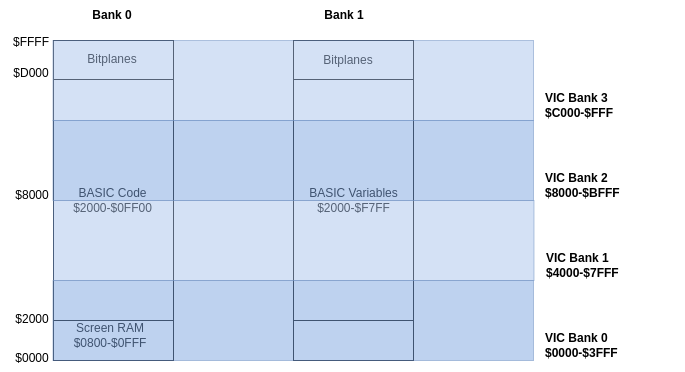
\includegraphics[width=\linewidth]{images/graphics/vic-banks.png}

Independent of the VIC, the memory management of the Commodore 65 or MEGA65 is somewhat more complex than that of the previous model. This is because there is more memory available in the machine: For the Commodore 65 128KB where planned (potentially expandable to 1MB), while the MEGA65 comes with 384KB of chip RAM + 8MB of attic RAM (potentially expandable to 256MB). As already mentioned, the processor is not able to address the whole range of memory. Only 64KB can be seen. For this reason, the memory is divided into blocks, 64KB each, and these blocks are called "banks".

The system can have up to 16 banks and certain banks also have certain tasks. Banks 0 and 1 are RAM, which means you can read and write to them, while banks 2 and 3 are ROM and not so easy to override.

Bank 0 (from the perspective of the BASIC 65 operating system that runs when you power the system on) is called the system bank. It contains regions such as:

\begin{itemize}
  \item The screen RAM, which occupies the memory range \$0800-\$2000 (by default)
  \item Memory-mapped VIC registers (if they have been mapped in, and by default, they are)
\end{itemize}

By the way, the BASIC65 implementation itself is stored in ROM (bank 3), while the C64's BASIC is also stored in ROM (bank 2).

If you want to know more about memory management in general please have a look at \bookvref{cha:memory-map}. In BASIC - sorry to say - the situation gets even more complex. Right after turning on the computer you are in Bank 128 which is a special bank with a special memory configuration. You can use the command BANK to switch between banks. A problem here is, that you can easily lose track of what is in which bank or in which bank you are currently working. It's actually a bit easier when working in machine language. For more information about the BANK-command and banks in general, please look into \bookvref{BASIC 65 Commands!BANK}. Please keep in mind that you need to know about banks before you can safely use PEEK, POKE or SYS. Otherwise you may wonder why your program does not behave as expected. We will come back to this later. Back to graphics.

Let's begin to write a simple BASIC program to show hires bitmap graphics. If you followed this chapter carefully up to this point, you should have no trouble understanding the following lines of code:

\begin{screencode}
10 POKE $D020,0 : POKE $D021,0          :REM MAKE SCREEN BLACK
20 POKE $D031, PEEK($D031) AND 127      :REM SET RESOLUTION
30 POKE $DD02, 3                        :REM MAKE VIRTUAL CIA-2 READ- AND WRITEABLE
40 POKE $$DD00, PEEK($DD00) AND 252 OR 2:REM SELECT VIDEO BANK 1
\end{screencode}

As you have seen in the illustration on the page before, the VIC chip divides the memory into 4 video banks of 16KB each. It is important to understand that you do not use a register of the VIC to define the video bank inside the (memory-)bank 0, instead you use the data bits 0 and 1 of \$DD00 or 56576 decimal. This used to be a register of the CIA-2 chip on the Commodore 64 but in your MEGA65 it is implemented as a virtual register. The "preparation" needed to set the video bank happens in line 30 while in the following line the video bank itself is set. By the way, when you convert the decimal value 3 (line 30) into its binary format, it is 00000011 and proves: the data bits 0 and 1 are set to 1, so reading and writing is activated.

\begin{tabular}{|c|c|l|l|}
	\hline
	Bits & VIC bank & Memory Area & BASIC \\
	\hline
	 \textbf{00} & 3 & \$C000-\$FFFF & ... AND 252 OR 0 :REM AND 11111100 OR 000000\textbf{00} \\
	 \textbf{01} & 2 & \$8000-\$BFFF & ... AND 252 OR 1 :REM AND 11111100 OR 000000\textbf{01} \\
	 \textbf{10} & 1 & \$4000-\$7FFF & ... AND 252 OR 2 :REM AND 11111100 OR 000000\textbf{10} \\
	 \textbf{11} & 0 & \$0000-\$3FFF & ... AND 252 OR 3 :REM AND 11111100 OR 000000\textbf{11} \\
	\hline
\end{tabular}

The table shows which bits must be set to select a video bank.

%\input{sprites}
%\input{sound}

%\part{APPENDICES}

\begin{appendices}

  \def\drivedefinition{
{\bf drive} drive \# in dual drive disk units. \\
The drive \# defaults to {\bf 0} and can be omitted on single drive units
such as the 1541, 1571, or 1581.
}

\def\unitdefinition{
{\bf unit} device number on the IEC bus.
Typically in the range from 8 to 11 for disk units.
If a variable is used, it must be placed in brackets.
The unit \# defaults to {\bf 8}.
}

\def\filenamedefinition{
{\bf filename} the name of a file. Either a quoted string such as \screentext{"DATA"}, or
a string expression in brackets such as \screentext{(FI\$)}.
}

\def\dirnamedefinition{
{\bf dirname} the name of a directory. Either a quoted string such as \screentext{"SOMEDIR"}, or
a string expression in brackets such as \screentext{(DR\$)}.
}

  \input{appendix-basic65-condensed}
  \chapter{Special Keyboard Controls and Sequences}


\section{PETSCII Codes and CHR\$}

\label{appendix:asciicodes}

In BASIC,  \screentext{PRINT CHR\$(X)} can be used to print a character from a PETSCII code.
Below is the full table of PETSCII codes you can print by index.  For example, while in the default uppercase/graphics mode, by
using index 65 from the table below as: \screentext{PRINT CHR\$(65)} you will
print the letter \screentext{A}. You can read more about {\bf CHR\$} on page \pageref{chrcommand}.

You can also do the reverse with the ASC statement.  For example:
\screentext{PRINT ASC("A")} will output \screentext{65}, which matches the
code in the table.

\underline{Note}: Function key (F1-F14 + HELP) values in this table are not intended to be printed via \screentext{CHR\$()},
but rather to allow function-key input to be assessed in BASIC programs via the GET / GETKEY commands.

\index{Keyboard!PETSCII Codes and CHR\$}
\begin{adjustwidth}{}{-2cm}
\begin{multicols}{4}
\begin{description}[align=left,labelwidth=0.2cm]
    \item [0]
    \item [1]   \small{ALTERNATE PALETTE}
    \item [2]   \small{UNDERLINE ON}
    \item [3]
    \item [4]   \small{DEFAULT PALETTE}
    \item [5]   \small{WHITE}
    \item [6]
    \item [7]   \small{BELL}
    \item [8]
    \item [9]   \specialkey{TAB}
    \item [10]  \small{LINEFEED}
%   \item [11]  \footnotesize{DISABLE \specialkey{SHIFT}\megasymbolkey}
    \item [11]  DISABLE \\ \specialkey{SHIFT}\megasymbolkey
%   \item [12]  \footnotesize{ENABLE \specialkey{SHIFT}\megasymbolkey}
    \item [12]  ENABLE \\ \specialkey{SHIFT}\megasymbolkey
    \item [13]  \specialkey{RETURN}
    \item [14]  \small{LOWER CASE}
    \item [15]  \small{BLINK/FLASH ON}
    \item [16]  F9
    \item [17]  \megakey{$\downarrow$}
    \item [18]  \specialkey{RVS ON}
    \item [19]  \specialkey{CLR HOME}
    \item [20]  \specialkey{INST DEL}
    \item [21]  F10 / BACK WORD
    \item [22]  F11
    \item [23]  F12 / NEXT WORD
    \item [24]  SET/CLEAR TAB
    \item [25]  F13
    \item [26]  F14 / BACK TAB
    \item [27]  \small{ESCAPE}
    \item [28]  \small{RED}
    \item [29]  \megakey{$\rightarrow$}
    \item [30]  \small{GREEN}
    \item [31]  \small{BLUE}
    \item [32]  \megakey{SPACE}
    \item [33]  !
    \item [34]  "
    \item [35]  \#
    \item [36]  \$
    \item [37]  \%
    \item [38]  \&
    \item [39]  '
    \item [40]  (
    \item [41]  )
    \item [42]  *
    \item [43]  +
    \item [44]  ,
    \item [45]  -
    \item [46]  .
    \item [47]  /
    \item [48]  0
    \item [49]  1
    \item [50]  2
    \item [51]  3
    \item [52]  4
    \item [53]  5
    \item [54]  6
    \item [55]  7
    \item [56]  8
    \item [57]  9
    \item [58]  :
    \item [59]  ;
    \item [60]  <
    \item [61]  =
    \item [62]  >
    \item [63]  ?
    \item [64]  @
    \item [65]  A
    \item [66]  B
    \item [67]  C
    \item [68]  D
    \item [69]  E
    \item [70]  F
    \item [71]  G
    \item [72]  H
    \item [73]  I
    \item [74]  J
    \item [75]  K
    \item [76]  L
    \item [77]  M
    \item [78]  N
    \item [79]  O
    \item [80]  P
    \item [81]  Q
    \item [82]  R
    \item [83]  S
    \item [84]  T
    \item [85]  U
    \item [86]  V
    \item [87]  W
    \item [88]  X
    \item [89]  Y
    \item [90]  Z
    \item [91]  [
    \item [92]  \pounds
    \item [93]  ]
    \item [94]  \megakeywhite{$\uparrow$}
    \item [95]  \megakeywhite{$\leftarrow$}
    \item [96]  \graphicsymbol{C}
    \item [97]  \graphicsymbol{A}
    \item [98]  \graphicsymbol{B}
    \item [99]  \graphicsymbol{C}
    \item [100] \graphicsymbol{D}
    \item [101] \graphicsymbol{E}
    \item [102] \graphicsymbol{F}
    \item [103] \graphicsymbol{G}
    \item [104] \graphicsymbol{H}
    \item [105] \graphicsymbol{I}
    \item [106] \graphicsymbol{J}
    \item [107] \graphicsymbol{K}
    \item [108] \graphicsymbol{L}
    \item [109] \graphicsymbol{M}
    \item [110] \graphicsymbol{N}
    \item [111] \graphicsymbol{O}
    \item [112] \graphicsymbol{P}
    \item [113] \graphicsymbol{Q}
    \item [114] \graphicsymbol{R}
    \item [115] \graphicsymbol{S}
    \item [116] \graphicsymbol{T}
    \item [117] \graphicsymbol{U}
    \item [118] \graphicsymbol{V}
    \item [119] \graphicsymbol{W}
    \item [120] \graphicsymbol{X}
    \item [121] \graphicsymbol{Y}
    \item [122] \graphicsymbol{Z}
    \item [123] \graphicsymbol{+}
    \item [124] \graphicsymbol{-}
    \item [125] \graphicsymbol{B}
    \item [126] \graphicsymbol{\textbackslash}
    \item [127] \graphicsymbol{]}
    \item [128]
    \item [129] \small{ORANGE}
    \item [130] \small{UNDERLINE OFF}
    \item [131]
    \item [132] HELP
    \item [133] F1
    \item [134] F3
    \item [135] F5
    \item [136] F7
    \item [137] F2
    \item [138] F4
    \item [139] F6
    \item [140] F8
    \item [141] \specialkey{SHIFT}\specialkey{RETURN}
    \item [142] \small{UPPERCASE}
    \item [143] \small{BLINK/FLASH OFF}
    \item [144] \small{BLACK}
    \item [145] \megakey{$\uparrow$}
    \item [146] \specialkey{RVS OFF}
    \item [147] \specialkey{SHIFT}\specialkey{CLR HOME}
    \item [148] \specialkey{SHIFT}\specialkey{INST DEL}
    \item [149] \small{BROWN}
    \item [150] \small{PINK}
    \item [151] \small{DK. GREY}
    \item [152] \small{GREY}
    \item [153] \small{LT. GREEN}
    \item [154] \small{LT. BLUE}
    \item [155] \small{LT. GREY}
    \item [156] \small{PURPLE}
    \item [157] \megakey{$\leftarrow$}
    \item [158] \small{YELLOW}
    \item [159] \small{CYAN}
    \item [160] \megakey{SPACE}
    \item [161] \graphicsymbol{k}
    \item [162] \graphicsymbol{i}
    \item [163] \graphicsymbol{t}
    \item [164] \graphicsymbol{[}
    \item [165] \graphicsymbol{g}
    \item [166] \graphicsymbol{=}
    \item [167] \graphicsymbol{m}
    \item [168] \graphicsymbol{/}
    \item [169] \graphicsymbol{?}
    \item [170] \graphicsymbol{v}
    \item [171] \graphicsymbol{q}
    \item [172] \graphicsymbol{d}
    \item [173] \graphicsymbol{z}
    \item [174] \graphicsymbol{s}
    \item [175] \graphicsymbol{n}
    \item [176] \graphicsymbol{a}
    \item [177] \graphicsymbol{e}
    \item [178] \graphicsymbol{r}
    \item [179] \graphicsymbol{w}
    \item [180] \graphicsymbol{h}
    \item [181] \graphicsymbol{j}
    \item [182] \graphicsymbol{l}
    \item [183] \graphicsymbol{y}
    \item [184] \graphicsymbol{u}
    \item [185] \graphicsymbol{p}
    \item [186] \graphicsymbol{\{}
    \item [187] \graphicsymbol{f}
    \item [188] \graphicsymbol{c}
    \item [189] \graphicsymbol{x}
    \item [190] \graphicsymbol{v}
    \item [191] \graphicsymbol{b}
\end{description}
\end{multicols}
\end{adjustwidth}

\underline{Note 1}: Codes from 192 to 223 are equal to 96 to 127. Codes from 224 to 254 are equal to 160 to 190,
and code 255 is equal to 126.

\underline{Note 2}: While using lowercase/uppercase mode (by pressing \megasymbolkey + \specialkey{SHIFT}), be aware that:
\begin{itemize}
  \item The uppercase letters in region 65-90 of the above table are replaced with lowercase letters.
  \item The graphical characters in region 97-122 of the above table are replaced with uppercase letters.
  \item PETSCII's lowercase (65-90) and uppercase (97-122) letters are in ASCII's uppercase (65-90) and lowercase (97-122) letter regions.
\end{itemize}


\section{Control codes}
\label{appendix:controlcodes}
\index{Keyboard!CTRL}
\begin{center}
\setlength{\def\arraystretch{1.5}\tabcolsep}{6pt}
\begin{longtable}{c|L{5.5cm}}
	\textbf{Keyboard Control} & \textbf{Function}\\
   \hhline{==}
	\endhead

  \multicolumn{2}{l}{\textbf{Colours}} \\
  \hhline{==}
\specialkey{CTRL} + \megakey{1} to \megakey{8} &
Choose from the first range of colours. More information on the colours
    available is under the BASIC {\bf BACKGROUND} command on page \pageref{colourtable}.\\
\hline
\megasymbolkey + \megakey{1} to \megakey{8} &
Choose from the second range of colours.  \\
\hline
\specialkey{CTRL} + \megakey{E} &
Restores the colour of the cursor back to the default (white).\\
\hline
\specialkey{CTRL} + \megakey{D} &
Switches the VIC-IV to colour range 0-15 (default colours). These colours can be accessed with \specialkey{CTRL} and keys \megakey{1} to \megakey{8} (for the first 8 colours), or \megasymbolkey and keys \megakey{1} to \megakey{8} (for the remaining 8 colours).\\
\hline
\specialkey{CTRL} + \megakey{A} &
Switches the VIC-IV to colour range 16-31 (alternate/rainbow colours). These colours can be accessed with \specialkey{CTRL} and keys \megakey{1} to \megakey{8} (for the first 8 colours), or \megasymbolkey and keys \megakey{1} to \megakey{8} (for the remaining 8 colours).\\
  \hhline{==}
  \multicolumn{2}{l}{\textbf{Tabs}} \\
  \hhline{==}
\specialkey{CTRL} + \megakey{Z} &
Tabs the cursor to the left. If there are no tab positions remaining, the cursor will remain at the start of the line.\\
\hline
\specialkey{CTRL} + \megakey{I} &
Tabs the cursor to the right. If there are no tab positions remaining, the cursor will remain at the end of the line.\\
\hline
\specialkey{CTRL} + \megakey{X} &
Sets or clears the current screen column as a tab position.
 Use \specialkey{CTRL} +\megakey{Z} and \megakey{I}  to jump back and forth to all positions set with \megakey{X}.\\
  \hhline{==}
  \multicolumn{2}{l}{\textbf{Movement}} \\
  \hhline{==}
\specialkey{CTRL} + \megakey{Q} &
Moves the cursor down one line at a time. Equivalent to \megakey{$\downarrow$}.\\
\hline
\specialkey{CTRL} + \megakey{J} &
Moves the cursor down a position. If you are on a long line of BASIC code that has extended to two lines, then the cursor will move down two rows to be on the next line.\\
\hline
\specialkey{CTRL} + \megakey{]} &
Equivalent to \megakey{$\rightarrow$}.\\
\hline
\specialkey{CTRL} + \megakey{T} &
Backspace the character immediately to the left and to shift all rightmost characters one position to the left. This is equivalent to \specialkey{INST DEL}.\\
\hline
\specialkey{CTRL} + \megakey{M} &
Performs a carriage return, equivalent to \specialkey{RETURN}.\\

  \hhline{==}
  \multicolumn{2}{l}{\textbf{Word movement}} \\
  \hhline{==}

\specialkey{CTRL} + \megakey{U} &
Moves the cursor back to the start of the previous word. If there are no words
between the current cursor position and the start of the line, the cursor will move to the first column of the current line.\\
\hline
\specialkey{CTRL} + \megakey{W} &
Advances the cursor forward to the start of the next word. If there are no words between the cursor and the end of the line,
the cursor will move to the first column of the next line.\\

  \hhline{==}
  \multicolumn{2}{l}{\textbf{Scrolling}} \\
  \hhline{==}

\specialkey{CTRL} + \megakey{P} &
Scroll BASIC listing down one line. Equivalent to \megakey{F9}.\\
\hline
\specialkey{CTRL} + \megakey{V} &
Scroll BASIC listing up one line. Equivalent to \megakey{F11}.\\
\hline
\specialkey{CTRL} + \megakey{S} &
Equivalent to \specialkey{NO\\SCROLL}.\\

  \hhline{==}
  \multicolumn{2}{l}{\textbf{Formatting}} \\
  \hhline{==}

\specialkey{CTRL} + \megakey{B} &
Enables underline text mode. You can disable underline mode by pressing \specialkey{ESC}, then \megakey{O}.\\
\hline
\specialkey{CTRL} + \megakey{O} &
Enables flashing text mode. You can disable flashing mode by pressing \specialkey{ESC}, then \megakey{O}.\\
\hline

  \hhline{==}
  \multicolumn{2}{l}{\textbf{Casing}} \\
  \hhline{==}

\specialkey{CTRL} + \megakey{N} &
Changes the text case mode from uppercase to lowercase.\\
\hline
\specialkey{CTRL} + \megakey{K} &
Locks the uppercase/lowercase mode switch usually performed with \megasymbolkey + \specialkey{SHIFT}.\\
\hline
\specialkey{CTRL} + \megakey{L} &
Enables the uppercase/lowercase mode switch that is performed with the \megasymbolkey + \specialkey{SHIFT}.\\

  \hhline{==}
  \multicolumn{2}{l}{\textbf{Miscellaneous}} \\
  \hhline{==}

\specialkey{CTRL} + \megakey{G} &
Produces a bell tone.\\
\hline
\specialkey{CTRL} + \megakey{[} &
Equivalent to pressing \specialkey{ESC}.\\
\hline
\specialkey{CTRL} + \megakey{*} &
Enters the Matrix Mode Debugger.\\
\hline

\end{longtable}
\end{center}


\section{Shifted codes}
\label{appendix:shiftedcodes}
\index{Keyboard!Shift Keys}
\begin{center}
\setlength{\def\arraystretch{1.5}\tabcolsep}{6pt}
\begin{longtable}{c|L{5.5cm}}
	\textbf{Keyboard Control} & \textbf{Function}\\
  \hhline{==}
	\endhead

\specialkey{SHIFT} + \specialkey{INST DEL} &
Insert a character at the current cursor position and move all characters to the right by one position.\\
\hline
\specialkey{SHIFT} + \specialkey{HOME} &
Clear home, clear the entire screen, and move the cursor to the home position.\\
\hline

\end{longtable}
\end{center}



\section{Escape Sequences}
\label{escape-sequences}
\index{Keyboard!Escape Sequences}
To perform an Escape Sequence, press and release \specialkey{ESC},
then press one of the following keys to perform the sequence:

\begin{center}
\setlength{\def\arraystretch{1.5}\tabcolsep}{6pt}
\begin{longtable}{c|L{5.5cm}}
	\textbf{Key} & \textbf{Sequence}\\
  \hhline{==}
	\endhead

  \multicolumn{2}{l}{\textbf{Editor behaviour}} \\
  \hhline{==}

\specialkey{ESC} \megakey{X} &
Clears the screen and toggles between 40 and 80-column modes.\\
\hline

\specialkey{ESC} \megakey{4} &
Clears the screen and switches to 40 column mode.\\
\hline

\specialkey{ESC} \megakey{8} &
Clears the screen and switches to 80 column mode.\\
\hline

\specialkey{ESC} \megakey{@} &
%TODO the megakey with @ shows the label far smaller than any other key.
% Perhaps it needs more styling?
Clears a region of the screen, starting from the current cursor position, to the end of the screen.\\
\hline

\specialkey{ESC} \megakey{O} &
Cancels the quote, reverse, underline, and flash modes.\\

  \hhline{==}
  \multicolumn{2}{l}{\textbf{Scrolling}} \\
  \hhline{==}
% TODO for some reason this doesn't leave enough space (the keys overlap with the hhline)
\specialkey{ESC} \megakey{V} &
Scrolls the entire screen up one line.\\
\hline
\specialkey{ESC} \megakey{W} &
Scrolls the entire screen down one line.\\
\hline
\specialkey{ESC} \megakey{L} &
Enables scrolling when \megakey{$\downarrow$} is pressed at the bottom of the screen.\\
\hline
\specialkey{ESC} \megakey{M} &
Disables scrolling. When pressing \megakey{$\downarrow$} at the bottom of the screen, the cursor will move to the top of the
screen. However, when pressing \megakey{$\uparrow$} at the top of the screen, the cursor will remain on the first line.\\
  \hhline{==}
  \multicolumn{2}{l}{\textbf{Insertion and deletion}} \\
  \hhline{==}
\specialkey{ESC} \megakey{I} &
Inserts an empty line at the current cursor position and moves all subsequent lines down one position.\\
\hline
\specialkey{ESC} \megakey{D} &
Deletes the current line and moves lines below the cursor up one position.\\
\hline
\specialkey{ESC} \megakey{P} &
Erases all characters from the cursor to the start of the current line.\\
\hline
\specialkey{ESC} \megakey{Q} &
Erases all characters from the cursor to the end of the current line.\\
  \hhline{==}
  \multicolumn{2}{l}{\textbf{Movement}} \\
  \hhline{==}
\specialkey{ESC} \megakey{J} &
Moves the cursor to the start of the current line.\\
\hline
\specialkey{ESC} \megakey{K} &
Moves the cursor to the last non-whitespace character on the current line.\\
\hline
\specialkey{ESC} \megakeywhite{$\uparrow$} &
\index{Keyboard!Cursor Keys}
Saves the current cursor position. Use \specialkey{ESC} \megakeywhite{$\leftarrow$} (next to \megakey{1}) to move it
    back
to the saved position. Note that the \megakeywhite{$\uparrow$} used here is next to \widekey{RESTORE}.\\
\hline
\specialkey{ESC} \megakeywhite{$\leftarrow$} &
Restores the cursor position to the position stored via a prior a press of the \specialkey{ESC}
    \megakeywhite{$\uparrow$}
(next to \widekey{RESTORE}) key sequence. Note that the \megakeywhite{$\leftarrow$} used here is next to \megakey{1}.\\
\hline
\specialkey{ESC} \specialkey{HOME} &
Restores the cursor position to the position stored via a prior a press of \specialkey{HOME}.\\

  \hhline{==}
  \multicolumn{2}{l}{\textbf{Windowing}} \\
  \hhline{==}
\specialkey{ESC} \megakey{T} &
Sets the top-left corner of the windowed area.
All typed characters and screen activity will be restricted to the area. Also see \specialkey{ESC} \megakey{B}.
Windowed mode can be disabled by pressing \specialkey{CLR HOME} twice. \\
\hline
\specialkey{ESC} \megakey{B} &
Sets the bottom right corner of the windowed area.
All typed characters and screen activity will be restricted to the area. Also see \specialkey{ESC} \megakey{T}.
Windowed mode can be disabled by pressing \specialkey{CLR HOME} twice.\\
  \hhline{==}
  \multicolumn{2}{l}{\textbf{Cursor behaviour}} \\
  \hhline{==}
\specialkey{ESC} \megakey{A} &
Enables auto-insert mode. Any keys pressed will be inserted at the current cursor position, shifting all characters
on the current line after the cursor to the right by one position.\\
\hline
\specialkey{ESC} \megakey{C} &
Disables auto-insert mode, reverting back to overwrite mode.\\
\hline
\specialkey{ESC} \megakey{E} &
Sets the cursor to non-flashing mode.\\
\hline
\specialkey{ESC} \megakey{F} &
Sets the cursor to regular flashing mode.\\
  \hhline{==}
  \multicolumn{2}{l}{\textbf{Bell behaviour}} \\
  \hhline{==}
\specialkey{ESC} \megakey{G} &
Enables the bell which can be sounded using \specialkey{CTRL} and \megakey{G}.\\
\hline
\specialkey{ESC} \megakey{H} &
Disable the bell so that pressing \specialkey{CTRL} and \megakey{G} will have no effect.\\
  \hhline{==}
  \multicolumn{2}{l}{\textbf{Colours}} \\
  \hhline{==}
\specialkey{ESC} \megakey{U} &
\label{appendix:escape-colours}
Switches the VIC-IV to colour range 0-15 (default colours). These colours can be accessed with \specialkey{CTRL} and keys \megakey{1} to \megakey{8} (for the first 8 colours), or \megasymbolkey and keys \megakey{1} to \megakey{8} (for the remaining colours).\\
\hline
\specialkey{ESC} \megakey{S} &
Switches the VIC-IV to colour range 16-31 (alternate/rainbow colours). These colours can be accessed with \specialkey{CTRL} and keys \megakey{1} to \megakey{8} (for the first 8 colours), or \megasymbolkey and keys \megakey{1} to \megakey{8} (for the remaining colours).\\
\hline
  \hhline{==}
  \multicolumn{2}{l}{\textbf{Tabs}} \\
  \hhline{==}
\specialkey{ESC} \megakey{Y} &
Set the default tab stops (every 8 spaces) for the entire screen.\\
\hline
\specialkey{ESC} \megakey{Z} &
Clears all tab stops. Any tabbing with \specialkey{CTRL} and \megakey{I} will move the cursor to the end of the line.\\
\hline
\end{longtable}
\end{center}

  \chapter{Screen Editor Keys}

\section{Screen Editor Keys}

The following key combinations perform actions in the MEGA65 screen editor.

In some cases, a program can print the equivalent PETSCII codes to perform the same actions. For example, \specialkey{CTRL} + \megakey{G}, which plays a bell sound, can be printed by a program as \screentext{CHR\$(7)}. To print an \specialkey{ESC} sequence, use \screentext{CHR\$(27)} to represent the \specialkey{ESC} key, followed by the next key in the sequence.

\section{Control codes}
\label{appendix:controlcodes}
\index{Keyboard!CTRL}
\begin{center}
\setlength{\def\arraystretch{1.5}\tabcolsep}{6pt}
\begin{longtable}{c|L{5.5cm}}
	\textbf{Keyboard Control} & \textbf{Function}\\
   \hhline{==}
	\endhead

  \multicolumn{2}{l}{\textbf{Colours}} \\
  \hhline{==}
\specialkey{CTRL} + \megakey{1} to \megakey{8} &
Choose from the first range of colours. See appendix \vref{appendix:colourtable} for the list of colours in the system palette.\\
\hline
\megasymbolkey + \megakey{1} to \megakey{8} &
Choose from the second range of colours.  \\
\hline
\specialkey{CTRL} + \megakey{E} &
Restores the colour of the cursor back to the default (white).\\
\hline
\specialkey{CTRL} + \megakey{D} &
Switches the VIC-IV to colour range 0-15 (default colours). These colours can be accessed with \specialkey{CTRL} and keys \megakey{1} to \megakey{8} (for the first 8 colours), or \megasymbolkey and keys \megakey{1} to \megakey{8} (for the remaining 8 colours).\\
\hline
\specialkey{CTRL} + \megakey{A} &
Switches the VIC-IV to colour range 16-31 (alternate/rainbow colours). These colours can be accessed with \specialkey{CTRL} and keys \megakey{1} to \megakey{8} (for the first 8 colours), or \megasymbolkey and keys \megakey{1} to \megakey{8} (for the remaining 8 colours).\\
  \hhline{==}
  \multicolumn{2}{l}{\textbf{Tabs}} \\
  \hhline{==}
\specialkey{CTRL} + \megakey{Z} &
Tabs the cursor to the left. If there are no tab positions remaining, the cursor will remain at the start of the line.\\
\hline
\specialkey{CTRL} + \megakey{I} &
Tabs the cursor to the right. If there are no tab positions remaining, the cursor will remain at the end of the line.\\
\hline
\specialkey{CTRL} + \megakey{X} &
Sets or clears the current screen column as a tab position.
 Use \specialkey{CTRL} +\megakey{Z} and \megakey{I}  to jump back and forth to all positions set with \megakey{X}.\\
  \hhline{==}
  \multicolumn{2}{l}{\textbf{Movement}} \\
  \hhline{==}
\specialkey{CTRL} + \megakey{Q} &
Moves the cursor down one line at a time. Equivalent to \megakey{$\downarrow$}.\\
\hline
\specialkey{CTRL} + \megakey{J} &
Moves the cursor down a position. If you are on a long line of BASIC code that has extended to two lines, then the cursor will move down two rows to be on the next line.\\
\hline
\specialkey{CTRL} + \megakey{]} &
Equivalent to \megakey{$\rightarrow$}.\\
\hline
\specialkey{CTRL} + \megakey{T} &
Backspace the character immediately to the left and to shift all rightmost characters one position to the left. This is equivalent to \specialkey{INST DEL}.\\
\hline
\specialkey{CTRL} + \megakey{M} &
Performs a carriage return, equivalent to \specialkey{RETURN}.\\

  \hhline{==}
  \multicolumn{2}{l}{\textbf{Word movement}} \\
  \hhline{==}

\specialkey{CTRL} + \megakey{U} &
Moves the cursor backward to the start of the previous word. If there is no previous word on the current line, it moves to the first column of the current line, then to the previous line, until a line with a word is encountered.\\
\hline
\specialkey{CTRL} + \megakey{W} &
Advances the cursor forward to the start of the next word. If there is no next word on the current line, it moves to the first column of the next line, until a line with a word is encountered.\\

  \hhline{==}
  \multicolumn{2}{l}{\textbf{Scrolling}} \\
  \hhline{==}

\specialkey{CTRL} + \megakey{P} &
Scroll BASIC listing down one line. Equivalent to \megakey{F9}.\\
\hline
\specialkey{CTRL} + \megakey{V} &
Scroll BASIC listing up one line. Equivalent to \megakey{F11}.\\
\hline
\specialkey{CTRL} + \megakey{S} &
Equivalent to \specialkey{NO\\SCROLL}.\\

  \hhline{==}
  \multicolumn{2}{l}{\textbf{Formatting}} \\
  \hhline{==}

\specialkey{CTRL} + \megakey{B} &
Enables underline text mode. You can disable underline mode by pressing \specialkey{ESC}, then \megakey{O}.\\
\hline
\specialkey{CTRL} + \megakey{O} &
Enables flashing text mode. You can disable flashing mode by pressing \specialkey{ESC}, then \megakey{O}.\\
\hline

  \hhline{==}
  \multicolumn{2}{l}{\textbf{Casing}} \\
  \hhline{==}

\specialkey{CTRL} + \megakey{N} &
Changes the text case mode from uppercase to lowercase.\\
\hline
\specialkey{CTRL} + \megakey{K} &
Locks the uppercase/lowercase mode switch usually performed with \megasymbolkey + \specialkey{SHIFT}.\\
\hline
\specialkey{CTRL} + \megakey{L} &
Enables the uppercase/lowercase mode switch that is performed with the \megasymbolkey + \specialkey{SHIFT}.\\

  \hhline{==}
  \multicolumn{2}{l}{\textbf{Miscellaneous}} \\
  \hhline{==}

\specialkey{CTRL} + \megakey{G} &
Produces a bell tone.\\
\hline
\specialkey{CTRL} + \megakey{[} &
Equivalent to pressing \specialkey{ESC}.\\
\hline
\specialkey{CTRL} + \megakey{*} &
Enters the Matrix Mode Debugger.\\
\hline

\end{longtable}
\end{center}


\section{Shifted codes}
\label{appendix:shiftedcodes}
\index{Keyboard!Shift Keys}
\begin{center}
\setlength{\def\arraystretch{1.5}\tabcolsep}{6pt}
\begin{longtable}{c|L{5.5cm}}
	\textbf{Keyboard Control} & \textbf{Function}\\
  \hhline{==}
	\endhead

\specialkey{SHIFT} + \specialkey{INST DEL} &
Insert a character at the current cursor position and move all characters to the right by one position.\\
\hline
\specialkey{SHIFT} + \specialkey{HOME} &
Clear home, clear the entire screen, and move the cursor to the home position.\\
\hline

\end{longtable}
\end{center}



\section{Escape Sequences}
\label{escape-sequences}
\index{Keyboard!Escape Sequences}
To perform an Escape Sequence, briefly press and release \specialkey{ESC},
then press one of the following keys to perform the sequence.

\begin{center}
\setlength{\def\arraystretch{1.5}\tabcolsep}{6pt}
\begin{longtable}{c|L{5.5cm}}
	\textbf{Key} & \textbf{Sequence}\\
  \hhline{==}
	\endhead

  \multicolumn{2}{l}{\textbf{Editor behaviour}} \\
  \hhline{==}

\specialkey{ESC} \megakey{X} &
Clears the screen and toggles between 40 $\times$ 25 and 80 $\times$ 25 text modes.\\
\hline

\specialkey{ESC} \megakey{4} &
Clears the screen and switches to 40 $\times$ 25 text mode.\\
\hline

\specialkey{ESC} \megakey{8} &
Clears the screen and switches to 80 $\times$ 25 text mode.\\
\hline

\specialkey{ESC} \megakey{5} &
Switches to 80 $\times$ 50 text mode.\\
\hline
\multicolumn{2}{L{7cm}}{
  Note that some programs expect to be started in 80 $\times$ 25 mode,
  and may not behave correctly when started in 80 $\times$ 50 mode.} \\
\hline

\specialkey{ESC} \megakey{@} &
%TODO the megakey with @ shows the label far smaller than any other key.
% Perhaps it needs more styling?
Clears a region of the screen, starting from the current cursor position, to the end of the screen.\\
\hline

\specialkey{ESC} \megakey{O} &
Cancels the quote, reverse, underline, and flash modes.\\

  \hhline{==}
  \multicolumn{2}{l}{\textbf{Scrolling}} \\
  \hhline{==}
% TODO for some reason this doesn't leave enough space (the keys overlap with the hhline)
\specialkey{ESC} \megakey{V} &
Scrolls the entire screen up one line.\\
\hline
\specialkey{ESC} \megakey{W} &
Scrolls the entire screen down one line.\\
\hline
\specialkey{ESC} \megakey{L} &
Enables scrolling when \megakey{$\downarrow$} is pressed at the bottom of the screen.\\
\hline
\specialkey{ESC} \megakey{M} &
Disables scrolling. When pressing \megakey{$\downarrow$} at the bottom of the screen, the cursor will move to the top of the
screen. However, when pressing \megakey{$\uparrow$} at the top of the screen, the cursor will remain on the first line.\\
\hline
\specialkey{ESC} \megakey{N} &
Enables "line pushing:" typing or printing in the rightmost column pushes subsequent lines down by one.\\
\hline
\specialkey{ESC} \megakey{R} &
Disables "line pushing:" typing or printing in the rightmost column moves the cursor to the beginning of the next line, but does not push any lines. Disable both line pushing (\specialkey{ESC} \megakey{R}) and scrolling (\specialkey{ESC} \megakey{M}) to allow {\bf PRINT}ing in the rightmost column without disturbing the rest of the display.\\
\hhline{==}
  \multicolumn{2}{l}{\textbf{Insertion and deletion}} \\
  \hhline{==}
\specialkey{ESC} \megakey{I} &
Inserts an empty line at the current cursor position and moves all subsequent lines down one position.\\
\hline
\specialkey{ESC} \megakey{D} &
Deletes the current line and moves lines below the cursor up one position.\\
\hline
\specialkey{ESC} \megakey{P} &
Erases all characters from the cursor to the start of the current line.\\
\hline
\specialkey{ESC} \megakey{Q} &
Erases all characters from the cursor to the end of the current line.\\
  \hhline{==}
  \multicolumn{2}{l}{\textbf{Movement}} \\
  \hhline{==}
\specialkey{ESC} \megakey{J} &
Moves the cursor to the start of the current line.\\
\hline
\specialkey{ESC} \megakey{K} &
Moves the cursor to the last non-whitespace character on the current line.\\
\hline
\specialkey{ESC} \megakeywhite{$\uparrow$} &
\index{Keyboard!Cursor Keys}
Saves the current cursor position. Use \specialkey{ESC} \megakeywhite{$\leftarrow$} (next to \megakey{1}) to move it
    back
to the saved position. Note that the \megakeywhite{$\uparrow$} used here is next to \widekey{RESTORE}.\\
\hline
\specialkey{ESC} \megakeywhite{$\leftarrow$} &
Restores the cursor position to the position stored via a prior a press of the \specialkey{ESC}
    \megakeywhite{$\uparrow$}
(next to \widekey{RESTORE}) key sequence. Note that the \megakeywhite{$\leftarrow$} used here is next to \megakey{1}.\\
\hline
\specialkey{ESC} \specialkey{HOME} &
Restores the cursor position to the position stored via a prior a press of \specialkey{HOME}.\\

  \hhline{==}
  \multicolumn{2}{l}{\textbf{Windowing}} \\
  \hhline{==}
\specialkey{ESC} \megakey{T} &
Sets the top-left corner of the windowed area.
All typed characters and screen activity will be restricted to the area. Also see \specialkey{ESC} \megakey{B}.
Windowed mode can be disabled by pressing \specialkey{CLR HOME} twice. \\
\hline
\specialkey{ESC} \megakey{B} &
Sets the bottom right corner of the windowed area.
All typed characters and screen activity will be restricted to the area. Also see \specialkey{ESC} \megakey{T}.
Windowed mode can be disabled by pressing \specialkey{CLR HOME} twice.\\
  \hhline{==}
  \multicolumn{2}{l}{\textbf{Cursor behaviour}} \\
  \hhline{==}
\specialkey{ESC} \megakey{A} &
Enables auto-insert mode. Any keys pressed will be inserted at the current cursor position, shifting all characters
on the current line after the cursor to the right by one position.\\
\hline
\specialkey{ESC} \megakey{C} &
Disables auto-insert mode, reverting back to overwrite mode.\\
\hline
\specialkey{ESC} \megakey{E} &
Sets the cursor to non-flashing mode.\\
\hline
\specialkey{ESC} \megakey{F} &
Sets the cursor to regular flashing mode.\\
  \hhline{==}
  \multicolumn{2}{l}{\textbf{Bell behaviour}} \\
  \hhline{==}
\specialkey{ESC} \megakey{G} &
Enables the bell which can be sounded using \specialkey{CTRL} and \megakey{G}.\\
\hline
\specialkey{ESC} \megakey{H} &
Disable the bell so that pressing \specialkey{CTRL} and \megakey{G} will have no effect.\\
  \hhline{==}
  \multicolumn{2}{l}{\textbf{Colours}} \\
  \hhline{==}
\specialkey{ESC} \megakey{U} &
\label{appendix:escape-colours}
Switches the VIC-IV to colour range 0-15 (default colours). These colours can be accessed with \specialkey{CTRL} and keys \megakey{1} to \megakey{8} (for the first 8 colours), or \megasymbolkey and keys \megakey{1} to \megakey{8} (for the remaining colours).\\
\hline
\specialkey{ESC} \megakey{S} &
Switches the VIC-IV to colour range 16-31 (alternate/rainbow colours). These colours can be accessed with \specialkey{CTRL} and keys \megakey{1} to \megakey{8} (for the first 8 colours), or \megasymbolkey and keys \megakey{1} to \megakey{8} (for the remaining colours).\\
\hline
  \hhline{==}
  \multicolumn{2}{l}{\textbf{Tabs}} \\
  \hhline{==}
\specialkey{ESC} \megakey{Y} &
Set the default tab stops (every 8 spaces) for the entire screen.\\
\hline
\specialkey{ESC} \megakey{Z} &
Clears all tab stops. Any tabbing with \specialkey{CTRL} and \megakey{I} will move the cursor to the end of the line.\\
\hline
\end{longtable}
\end{center}

  \chapter{Screen Codes}

\section{Screen Codes}

\label{appendix:screencodes}

A text character is represented in screen memory by a screen code. There are
256 possible screen codes, each referring to an image in the current character
set.

A complete character set contains two groups of 256 images, one for the
uppercase mode and one for the lowercase mode, for a total of 512 images. Only
one mode can be displayed at a time. The built-in character sets use the first
128 characters of each group for normal characters and the next 128 for
reversed versions of the same characters.

In BASIC, the {\bf T@\&()} special array provides access to the characters on
the screen using column and row indexes. The values in this special array are
screen codes. The {\bf FONT} command changes between the built-in character
sets. The {\bf CHARDEF} command changes the image associated with a screen
code.

\underline{Note}: Screen codes are different to PETSCII codes. PETSCII codes
are used to store, transmit, and receive textual data, and control the way
strings are printed to the screen. When a PETSCII character is printed to the
screen, the corresponding screen code is written to screen memory. For a list
of PETSCII codes, see appendix \vref{appendix:asciicodes}.

The following table lists the screen codes. When a code produces a different
character based on the mode, the character is listed as ``uppercase /
lowercase.''

\index{Keyboard!Screen Codes}
\begin{adjustwidth}{}{-2cm}
\begin{multicols}{4}
\begin{description}[align=left,labelwidth=0.2cm]
    \item [0]   @
    \item [1]   A / a
    \item [2]   B / b
    \item [3]   C / c
    \item [4]   D / d
    \item [5]   E / e
    \item [6]   F / f
    \item [7]   G / g
    \item [8]   H / h
    \item [9]   I / i
    \item [10]  J / j
    \item [11]  K / k
    \item [12]  L / l
    \item [13]  M / m
    \item [14]  N / n
    \item [15]  O / o
    \item [16]  P / p
    \item [17]  Q / q
    \item [18]  R / r
    \item [19]  S / s
    \item [20]  T / t
    \item [21]  U / u
    \item [22]  V / v
    \item [23]  W / w
    \item [24]  X / x
    \item [25]  Y / y
    \item [26]  Z / z
    \item [27]  [
    \item [28]  \pounds
    \item [29]  ]
    \item [30]  $\uparrow$
    \item [31]  $\leftarrow$
    \item [32]  space
    \item [33]  !
    \item [34]  "
    \item [35]  \#
    \item [36]  \$
    \item [37]  \%
    \item [38]  \&
    \item [39]  '
    \item [40]  (
    \item [41]  )
    \item [42]  *
    \item [43]  +
    \item [44]  ,
    \item [45]  -
    \item [46]  .
    \item [47]  /
    \item [48]  0
    \item [49]  1
    \item [50]  2
    \item [51]  3
    \item [52]  4
    \item [53]  5
    \item [54]  6
    \item [55]  7
    \item [56]  8
    \item [57]  9
    \item [58]  :
    \item [59]  ;
    \item [60]  <
    \item [61]  =
    \item [62]  >
    \item [63]  ?
    \item [64]  \graphicsymbol{C}
    \item [65]  \graphicsymbol{A} / A
    \item [66]  \graphicsymbol{B} / B
    \item [67]  \graphicsymbol{C} / C
    \item [68]  \graphicsymbol{D} / D
    \item [69]  \graphicsymbol{E} / E
    \item [70]  \graphicsymbol{F} / F
    \item [71]  \graphicsymbol{G} / G
    \item [72]  \graphicsymbol{H} / H
    \item [73]  \graphicsymbol{I} / I
    \item [74]  \graphicsymbol{J} / J
    \item [75]  \graphicsymbol{K} / K
    \item [76]  \graphicsymbol{L} / L
    \item [77]  \graphicsymbol{M} / M
    \item [78]  \graphicsymbol{N} / N
    \item [79]  \graphicsymbol{O} / O
    \item [80]  \graphicsymbol{P} / P
    \item [81]  \graphicsymbol{Q} / Q
    \item [82]  \graphicsymbol{R} / R
    \item [83]  \graphicsymbol{S} / S
    \item [84]  \graphicsymbol{T} / T
    \item [85]  \graphicsymbol{U} / U
    \item [86]  \graphicsymbol{V} / V
    \item [87]  \graphicsymbol{W} / W
    \item [88]  \graphicsymbol{X} / X
    \item [89]  \graphicsymbol{Y} / Y
    \item [90]  \graphicsymbol{Z} / Z
    \item [91]  \graphicsymbol{+}
    \item [92]  \graphicsymbol{-}
    \item [93]  \graphicsymbol{B}
    \item [94]  \graphicsymbol{>}  %/ TODO: inverted checker
    \item [95]  \graphicsymbol{]} %/ TODO: back slashes
    \item [96]  space
    \item [97]  \graphicsymbol{j}
    \item [98]  \graphicsymbol{i}
    \item [99]  \graphicsymbol{t}
    \item [100] \graphicsymbol{[}
    \item [101] \graphicsymbol{g}
    \item [102] \graphicsymbol{=}
    \item [103] \graphicsymbol{m}
    \item [104] \graphicsymbol{/}
    \item [105] \graphicsymbol{?} %/ TODO: forward slashes
    \item [106] \graphicsymbol{n}
    \item [107] \graphicsymbol{q}
    \item [108] \graphicsymbol{d}
    \item [109] \graphicsymbol{z}
    \item [110] \graphicsymbol{s}
    \item [111] \graphicsymbol{p}
    \item [112] \graphicsymbol{a}
    \item [113] \graphicsymbol{e}
    \item [114] \graphicsymbol{r}
    \item [115] \graphicsymbol{w}
    \item [116] \graphicsymbol{h}
    \item [117] \graphicsymbol{j}
    \item [118] \graphicsymbol{l}
    \item [119] \graphicsymbol{y}
    \item [120] \graphicsymbol{u}
    \item [121] \graphicsymbol{p}
    \item [122] \graphicsymbol{\{} %/ TODO: checkmark
    \item [123] \graphicsymbol{f}
    \item [124] \graphicsymbol{c}
    \item [125] \graphicsymbol{x}
    \item [126] \graphicsymbol{v}
    \item [127] \graphicsymbol{b}
\end{description}
\end{multicols}
\end{adjustwidth}

\underline{Note}: In the built-in character sets, codes 128-255 are reversed versions of 0-127.

% TODO: Remove this once we have real images representing this.
\underline{Note}: In the lowercase group, 94 is an inverted version of \graphicsymbol{=}. 95 is a diagonal line pattern. 105 is the diagonal line pattern in the other direction. 122 is a checkmark.

  \chapter{Supporters \& Donors}


The MEGA65 would not have been possible to create without the generous support of many organisations and individuals.

We are still compiling these lists, so apologies if we haven't included you yet. If you know anyone we have left out, please let us know, so that we can recognise the contribution of everyone who has made the MEGA65 possible, and into the great retro-computing project that it has become.

\section{Organisations}

{\bf The MEGA Museum of Electronic Games \& Art e.V. Germany} \\
\megakey{Everything}

{\bf Trenz Electronic, Germany} \\
\megakey{Motherboard}
\megakey{Manufacturing}
\megakey{Sales}

{\bf Hintsteiner, Austria} \\
\megakey{Case}

{\bf GMK, Germany} \\
\megakey{Keyboard}

{\bf KEVAG Telekom, Germany} \\
\megakey{Web Hosting}

\newpage
\section{Contributors}

\begin{mega65thanks}

\begin{minipage}{\linewidth}
  {\large\bf Andreas Liebeskind} \\
  \textit{(libi in paradize)} \\
  CFO MEGA eV
\end{minipage}

\begin{minipage}{\linewidth}
  {\large\bf Thomas Hertzler} \\
  \textit{(grumpyninja)} \\
  USA spokesman
\end{minipage}

\begin{minipage}{\linewidth}
  {\large\bf Russell Peake} \\
  \textit{(rdpeake)} \\
  Bug herding
\end{minipage}

\begin{minipage}{\linewidth}
  {\large\bf Alexander Nik Petra} \\
  \textit{(n0d)} \\
  Early case design
\end{minipage}

\begin{minipage}{\linewidth}
  {\large\bf Ralph Egas} \\
  \textit{(0-limits)} \\
  Business advisor
\end{minipage}

\begin{minipage}{\linewidth}
  {\large\bf Lucas Moss} \\
  MEGAphone PCB design
\end{minipage}

\begin{minipage}{\linewidth}
  {\large\bf Daren Klamer} \\
  \textit{(Impakt)} \\
  Manual proof-reading
\end{minipage}

\begin{minipage}{\linewidth}
  {\large\bf Daniël Mantione}  \\
  \textit{(dmantione)} \\
  C64 hardware guru
\end{minipage}

\columnbreak

\begin{minipage}{\linewidth}
  {\large\bf Dr. Canan Hastik} \\
  \textit{(indica)} \\
  Chairwoman MEGA eV
\end{minipage}

\begin{minipage}{\linewidth}
  {\large\bf Simon Jameson} \\
  \textit{(Shallan)} \\
  Platform enhancements
\end{minipage}

\begin{minipage}{\linewidth}
  {\large\bf Stephan Kleinert} \\
  \textit{(ubik)} \\
  Destroyer of BASIC 10
\end{minipage}

\begin{minipage}{\linewidth}
  {\large\bf Wayne Johnson} \\
  \textit{(sausage)} \\
  Manual additions
\end{minipage}

\begin{minipage}{\linewidth}
  {\large\bf L. Kleiss} \\
  \textit{(LAK132)} \\
  MegaWAT presentation software
\end{minipage}

\begin{minipage}{\linewidth}
  {\large\bf Maurice van Gils }  \\
  \textit{(Maurice)}  \\
  BASIC 65 example programs
\end{minipage}

\begin{minipage}{\linewidth}
  {\large\bf Andrew Owen}  \\
  \textit{(Cheveron)} \\
  Keyboard, Sinclair support
\end{minipage}

\begin{minipage}{\linewidth}
  {\large\bf Adam Barnes}  \\
  \textit{(amb5l)} \\
  HDMI expert and board revision
\end{minipage}

\begin{minipage}{\linewidth}
  {\large\bf Wayne Rittimann, Jr.} \\
  \textit{(johnwayner)} \\
  Bug squashing on all levels
\end{minipage}

\end{mega65thanks}


\newpage
\section{Supporters}

\begin{small}
% page 1
\setlength{\tabcolsep}{1mm}
\begin{tabular}{p{4cm}p{4cm}p{4cm}}
3c74ce64 & Arne Neumann & Christian Gräfe \\
8-Bit Classics & Arne Richard Tyarks & Christian Heffner \\
@11110110100 & Axel Klahr & Christian Kersting \\
Aaron Smith & Balaz Ondrej & Christian Schiller \\
Achim Mrotzek & Barry Thompson & Christian Streck \\
Adolf Nefischer & Bartol Filipovic & Christian Weyer \\
Adrian Esdaile & Benjamin Maas & Christian Wyk \\
Adrien Guichard & Bernard Alaiz & Christoph Haug \\
Ahmed Kablaoui & Bernhard Zorn & Christoph Huck \\
Alan Bastian Witkowski & Bieno Marti-Braitmaier & Christoph Pross \\
Alan Field & Bigby & Christopher Christopher \\
Alastair Paulin-Campbell & Bill LaGrue & Christopher Kalk \\
Alberto Mercuri & Bjoerg Stojalowski & Christopher Kohlert \\
Alexander Haering & Björn Johannesson & Christopher Nelson \\
Alexander Kaufmann & Bjørn Melbøe & Christopher Taylor \\
Alexander Niedermeier & Bo Goeran Kvamme & Christopher Whillock \\
Alexander Soppart & Boerge Noest & Claudio Piccinini \\
Alfonso Ardire & Bolko Beutner & Claus Skrepek \\
Amiga On The Lake & Brett Hallen & Collen Blijenberg \\
André Kudra & Brian Gajewski & Constantine Lignos \\
André Simeit & Brian Green & Crnjaninja \\
André Wösten & Brian Juul Nielsen & Daniel Auger \\
Andrea Farolfi & Brian Reiter & Daniel Julien \\
Andrea Minutello & Bryan Pope & Daniel Lobitz \\
Andreas Behr & Burkhard Franke & Daniel O'Connor \\
Andreas Freier & Byron Goodman & Daniel Teicher \\
Andreas Grabski & Cameron Roberton (KONG) & Daniel Tootill \\
Andreas Millinger & Carl Angervall & Daniel Wedin \\
Andreas Nopper & Carl Danowski & Daniele Benetti \\
Andreas Ochs & Carl Stock & Daniele Gaetano Capursi \\
Andreas Wendel Manufaktur & Carl Wall & Dariusz Szczesniak \\
Andreas Zschunke & Carlo Pastore & Darrell Westbury \\
Andrew Bingham & Carlos Silva & David Asenjo Raposo \\
Andrew Dixon & Carsten Sørensen & David Dillard \\
Andrew Mondt & Cenk Miroglu Miroglu & David Gorgon \\
Andrzej Hłuchyj & Chang sik Park & David Norwood \\
Andrzej Sawiniec & Charles A. Hutchins Jr. & David Raulo \\
Andrzej Śliwa & Chris Guthrey & David Ross \\
Anthony W. Leal & Chris Hooper & de voughn accooe \\
Arkadiusz Bronowicki & Chris Stringer & Dean Scully \\
Arkadiusz Kwasny & Christian Boettcher & Dennis Jeschke \\
Arnaud Léandre & Christian Eick & Dennis Schaffers \\
Arne Drews & Christian Gleinser & Dennis Schierholz \\
\end{tabular}
% page 2
\newpage
\setlength{\tabcolsep}{1mm}
\begin{tabular}{p{4cm}p{4cm}p{4cm}}
Dennis Schneck & Frank Haaland & Helge Förster \\
denti & Frank Hempel & Hendrik Fensch \\
Dick van Ginkel & Frank Koschel & Henning Harperath \\
Diego Barzon & Frank Linhares & Henri Parfait \\
Dierk Schneider & Frank Sleeuwaert & Henrik Kühn \\
Dietmar Krueger & Frank Wolf & Holger Burmester \\
Dietmar Schinnerl & FranticFreddie & Holger Sturk \\
Dirk Becker & Fredrik Ramsberg & Howard Knibbs \\
Dirk Wouters & Fridun Nazaradeh & Hubert de Hollain \\
Domingo Fivoli & Friedel Kropp & Huberto Kusters \\
DonChaos & Garrick West & Hugo Maria Gerardus v.d. Aa \\
Donn Lasher & Gary Lake-Schaal & Humberto Castaneda \\
Douglas Johnson & Gary Pearson & Ian Cross \\
Dr. Leopold Winter & Gavin Jones & IDE64 Staff \\
Dusan Sobotka & Geir Sigmund Straume & Igor Ianov \\
Earl Woodman & Gerd Mitlaender & Igor Kurtes \\
Ed Reilly & Giampietro Albiero & Immo Beutler \\
Edoardo Auteri & Giancarlo Valente & Ingo Katte \\
Eduardo Gallardo & Gianluca Girelli & Ingo Keck \\
Eduardo Luis Arana & Giovanni Medina & Insanely Interested Publishing \\
Eirik Juliussen Olsen & Glen Fraser & IT-Dienstleistungen Obsieger \\
Emilio Monelli & Glen R Perye III & Ivan Elwood \\
EP Technical Services & Glenn Main & Jaap HUIJSMAN \\
Epic Sound & Gordon Rimac & Jace Courville \\
Erasmus Kuhlmann & GRANT BYERS & Jack Wattenhofer \\
ergoGnomik & Grant Louth & Jakob Schönpflug \\
Eric Hilaire & Gregor Bubek & Jakub Tyszko \\
Eric Hildebrandt & Gregor Gramlich & James Hart \\
Eric Hill & Guido Ling & James Marshburn \\
Eric Jutrzenka & Guido von Gösseln & James McClanahan \\
Erwin Reichel & Guillaume Serge & James Sutcliffe \\
Espen Skog & Gunnar Hemmerling & Jan Bitruff \\
Evangelos Mpouras & Günter Hummel & Jan Hildebrandt \\
Ewan Curtis & Guy Simmons & Jan Iemhoff \\
Fabio Zanicotti & Guybrush Threepwood & Jan Kösters \\
Fabrizio Di Dio & Hakan Blomqvist & Jan Peter Borsje \\
Fabrizio Lodi & Hans Pronk & Jan Schulze \\
FARA Gießen GmbH & Hans-Jörg Nett & Jan Stoltenberg-Lerche \\
FeralChild & Hans-Martin Zedlitz & Janne Tompuri \\
First Choice Auto's & Harald Dosch & Jannis Schulte \\
Florian Rienhardt & Harri Salokorpi & Jari Loukasmäki \\
Forum64. de & Harry Culpan & Jason Smith \\
Francesco Baldassarri & Harry Venema & Javier Gonzalez Gonzalez \\
Frank Fechner & Heath Gallimore & Jean-Paul Lauque \\
Frank Glaush & Heinz Roesner & Jeffrey van der Schilden \\
Frank Gulasch & Heinz Stampfli & Jens Schneider \\
\end{tabular}
% page 3
\newpage
\setlength{\tabcolsep}{1mm}
\begin{tabular}{p{4cm}p{4cm}p{4cm}}
Jens-Uwe Wessling & Kenneth Joensson & Marco Cappellari \\
Jesse DiSimone & Kevin Edwards & Marco Rivela \\
Jett Adams & Kevin Thomasson & Marco van de Water \\
Johan Arneklev & Kim Jorgensen & Marcus Gerards \\
Johan Berntsson & Kim Rene Jensen & Marcus Herbert \\
Johan Svensson & Kimmo Hamalainen & Marcus Linkert \\
Johannes Fitz & Konrad Buryło & Marek Pernicky \\
John Cook & Kosmas Einbrodt & Mario Esposito \\
John Deane & Kurt Klemm & Mario Fetka \\
John Dupuis & Lachlan Glaskin & Mario Teschke \\
John Nagi & Large bits collider & Mariusz Tymków \\
John Rorland & Lars Becker & Mark Adams \\
John Sargeant & Lars Edelmann & Mark Anderson \\
John Traeholt & Lars Slivsgaard & Mark Green \\
Jon Sandelin & Lasse Lambrecht & Mark Hucker \\
Jonas Bernemann & Lau Olivier & Mark Leitiger \\
Jonathan Prosise & Lee Chatt & Mark Spezzano \\
Joost Honig & Loan Leray & Mark Watkin \\
Jordi Pakey-Rodriguez & Lorenzo Quadri & Marko Rizvic \\
Jöre Weber & Lorenzo Travagli & Markus Bieler \\
Jörg Jungermann & Lorin Millsap & Markus Bonet \\
Jörg Schaeffer & Lothar James Foss & Markus Dauberschmidt \\
Jörg Weese & Lothar Serra Mari & Markus Fehr \\
Josef Hesse & Luca Papinutti & Markus Fuchs \\
Josef Soucek & Ludek Smetana & Markus Guenther-Hirn \\
Josef Stohwasser & Lukas Burger & Markus Liukka \\
Joseph Clifford & Lutz-Peter Buchholz & Markus Merz \\
Joseph Gerth & Luuk Spaetgens & Markus Roesgen \\
Jovan Crnjanin & Mad Web Skills & Markus Uttenweiler \\
Juan Pablo Schisano & MaDCz & Martin Bauhuber \\
Juan S. Cardona Iguina & Magnus Wiklander & Martin Benke \\
JudgeBeeb & Maik Diekmann & Martin Gendera \\
Juliussen Olsen & Malte Mundt & Martin Groß \\
Juna Luis Fernandez Garcia & Manfred Wittemann & Martin Gutenbrunner \\
Jürgen Endras & Manuel Beckmann & Martin Johansen \\
Jürgen Herm Stapelberg & Manzano Mérida & Martin Marbach \\
Jyrki Laurila & Marc "3D-vice" Schmitt & Martin Sonnleitner \\
Kai Pernau & Marc Bartel & Martin Steffen \\
Kalle Pöyhönen & Marc Jensen & Marvin Hardy \\
Karl Lamford & Marc Schmidt & Massimo Villani \\
Karl-Heinz Blum & Marc Theunissen & Mathias Dellacherie \\
Karsten Engstler & Marc Tutor & Mathieu Chouinard \\
Karsten Westebbe & Marc Wink & Matthew Adams \\
katarakt & Marcel Buchtmann & Matthew Browne \\
Keith McComb & Marcel Kante & Matthew Carnevale \\
Kenneth Dyke & Marco Beckers & Matthew Palmer \\
\end{tabular}
% page 4
\newpage
\setlength{\tabcolsep}{1mm}
\begin{tabular}{p{4cm}p{4cm}p{4cm}}
Matthew Santos & Michele Porcu & Paul Jackson \\
Matthias Barthel & Miguel Angel Rodriguez Jodar & Paul Johnson \\
Matthias Dolenc & Mikael Lund & Paul Kuhnast (mindrail) \\
Matthias Fischer & Mike Betz & Paul Massay \\
Matthias Frey & Mike Kastrantas & Paul Westlake \\
Matthias Grandis & Mike Pikowski & Paul Woegerer \\
Matthias Guth & Mikko Hämäläinen & Pauline Brasch \\
Matthias Lampe & Mikko Suontausta & Paulo Apolonia \\
Matthias Meier & Mirko Roller & Pete Collin \\
Matthias Mueller & Miroslav Karkus & Pete of Retrohax.net \\
Matthias Nofer & Morgan Antonsson & Peter Eliades \\
Matthias Schonder & Moritz & Peter Gries \\
Maurice Al-Khaliedy & Morten Nielsen & Peter Habura \\
Max Ihlenfeldt & MUBIQUO APPS,SL & Peter Herklotz \\
Meeso Kim & Myles Cameron-Smith & Peter Huyoff \\
Michael Dailly & Neil Moore & Peter Knörzer \\
Michael Dötsch & Nelson & Peter Leswell \\
Michael Dreßel & neoman & Peter Weile \\
Michael Fichtner & Nicholas Melnick & Petri Alvinen \\
Michael Fong & Nikolaj Brinch Jørgensen & Philip Marien \\
Michael Geoffrey Stone & Nils Andreas & Philip Timmermann \\
Michael Gertner & Nils Eilers & Philipp Rudin \\
Michael Grün & Nils Hammerich & Pierre Kressmann \\
Michael Habel & Nils77 & Pieter Labie \\
Michael Härtig & Norah Smith & Piotr Kmiecik \\
Michael Haynes & Norman King & Power-on.at \\
Michael J Burkett & Normen Zoch & Przemysław Safonow \\
Michael Jensen & Olaf Grunert & Que Labs \\
Michael Jurisch & Ole Eitels & R Welbourn \\
Michael Kappelgaard & Oliver Boerner & R-Flux \\
Michael Kleinschmidt & Oliver Brüggmann & Rafał Michno \\
Michael Lorenz & Oliver Graf & Rainer Kappler \\
Michael Mayerhofer & Oliver Smith & Rainer Kopp \\
Michael Nurney & Olivier Bori & Rainer Weninger \\
Michael Rasmussen & ONEPSI LLC & Ralf Griewel \\
Michael Richmond & oRdYNe & Ralf Pöscha \\
Michael Sachse & Osaühing Trioflex & Ralf Reinhardt \\
Michael Sarbak & OSHA-PROS USA & Ralf Schenden \\
Michael Schneider & Padawer & Ralf Smolarek \\
Michael Scholz & Patrick Becher & Ralf Zenker \\
Michael Timm & Patrick Bürckstümmer & Ralph Bauer \\
Michael Traynor & Patrick de Zoete & Ralph Wernecke \\
Michael Whipp & Patrick Toal & Rédl Károly \\
Michal Ursiny & Patrick Vogt & Reiner Lanowski \\
Michele Chiti & Paul Alexander Warren & Remi Veilleux \\
Michele Perini & Paul Gerhardt (KONG) & Riccardo Bianchi \\
\end{tabular}
% page 5
\newpage
\setlength{\tabcolsep}{1mm}
\begin{tabular}{p{4cm}p{4cm}p{4cm}}
Richard Englert & Sigurbjorn Larusson & Thomas Niemann \\
Richard Good & Sigurdur Finnsson & Thomas Scheelen \\
Richard Menedetter & Simon Lawrence & Thomas Schilling \\
Richard Sopuch & Simon Wolf & Thomas Tahsin-Bey \\
Rick Reynolds & spreen.digital & Thomas Walter \\
Rico Gruninger & Stefan Haberl & Thomas Wirtzmann \\
Rob Dean & Stefan Kramperth & Thorsten Knoll \\
Robert Bernardo & Stefan Richter & Thorsten Nolte \\
Robert Eaglestone & Stefan Schultze & Tim Krome \\
Robert Grasböck & Stefan Sonnek & Tim Waite \\
Robert Miles & Stefan Theil & Timo Weirich \\
Robert Schwan & Stefan Vrampe & Timothy Blanks \\
Robert Shively & Stefano Canali & Timothy Henson \\
Robert Tangmar & Stefano Mozzi & Timothy Prater \\
Robert Trangmar & Steffen Reiersen & Tobias Butter \\
Rodney Xerri & Stephan Bielmann & Tobias Heim \\
Roger Olsen & Stephen Jones & Tobias Köck \\
Roger Pugh & Stephen Kew & Tobias Lüthi \\
Roland Attila Kett & Steve Gray & Tommi Vasarainen \\
Roland Evers & Steve Kurlin & Toni Ammer \\
Roland Schatz & Steve Lemieux & Tore Olsen \\
Rolf Hass & Steven Combs & Torleif Strand \\
Ronald Cooper & Stewart Dunn & Torsten Schröder \\
Ronald Hunn & Stuart Marsh & Tuan Nguyen \\
Ronny Hamida & Sven Neumann & Uffe Jakobsen \\
Ronny Preiß & Sven Stache & Ulrich Hintermeier \\
Roy van Zundert & Sven Sternberger & Ulrich Nieland \\
Rüdiger Wohlfromm & Sven Wiegand & Ulrik Kruse \\
Ruediger Schlenter & Szabolcs Bence & Urban Lindeskog \\
Rutger WIllemsen & Tantrumedia Limited & Ursula Förstle \\
Sampo Peltonen & Techvana Operations Ltd. & Uwe Anfang \\
Sarmad Gilani & Teddy Turmeaux & Uwe Boschanski \\
SAS74 & Teemu Korvenpää & Vedran Vrbanc \\
Sascha Hesse & The Games Foundation & Verm Project \\
Scott Halman & Thierry Supplisson & Wayne Rittimann \\
Scott Hollier & Thieu-Duy Thai & Wayne Sander \\
Scott Robison & Thomas Bierschenk & Wayne Steele \\
Sebastian Baranski & Thomas Edmister & Who Knows \\
Sebastian Bölling & Thomas Frauenknecht & Winfried Falkenhahn \\
Sebastian Felzmann & Thomas Gitzen & Wolfgang Becker \\
Sebastian Lipp & Thomas Gruber & Wolfgang Stabla \\
Sebastian Rakel & Thomas Haidler & Worblehat \\
Şemseddin Moldibi & Thomas Jager & www.patop69.net \\
Seth Morabito & Thomas Karlsen & Yan B \\
Shawn McKee & Thomas Laskowski & Zoltan Markus \\
Siegfried Hartmann & Thomas Marschall & Zsolt Zsila \\
Zytex Online Store &  &  \\
\end{tabular}
\end{small}
\ifdefined\printmanual
\else
\setstretch{1}
\fi

\end{appendices}


\printindex

\pagestyle{empty}
\cleardoublepage

% Extra blank pages for printing:
\newpage\null\thispagestyle{empty}\newpage

\newpage
{\raggedright\huge\bf\color{headingblue} BASIC 65 QUICK REFERENCE CARD}
\vspace{12pt}
\\*

% Portrait orientation of Quick Reference for online viewing:
% 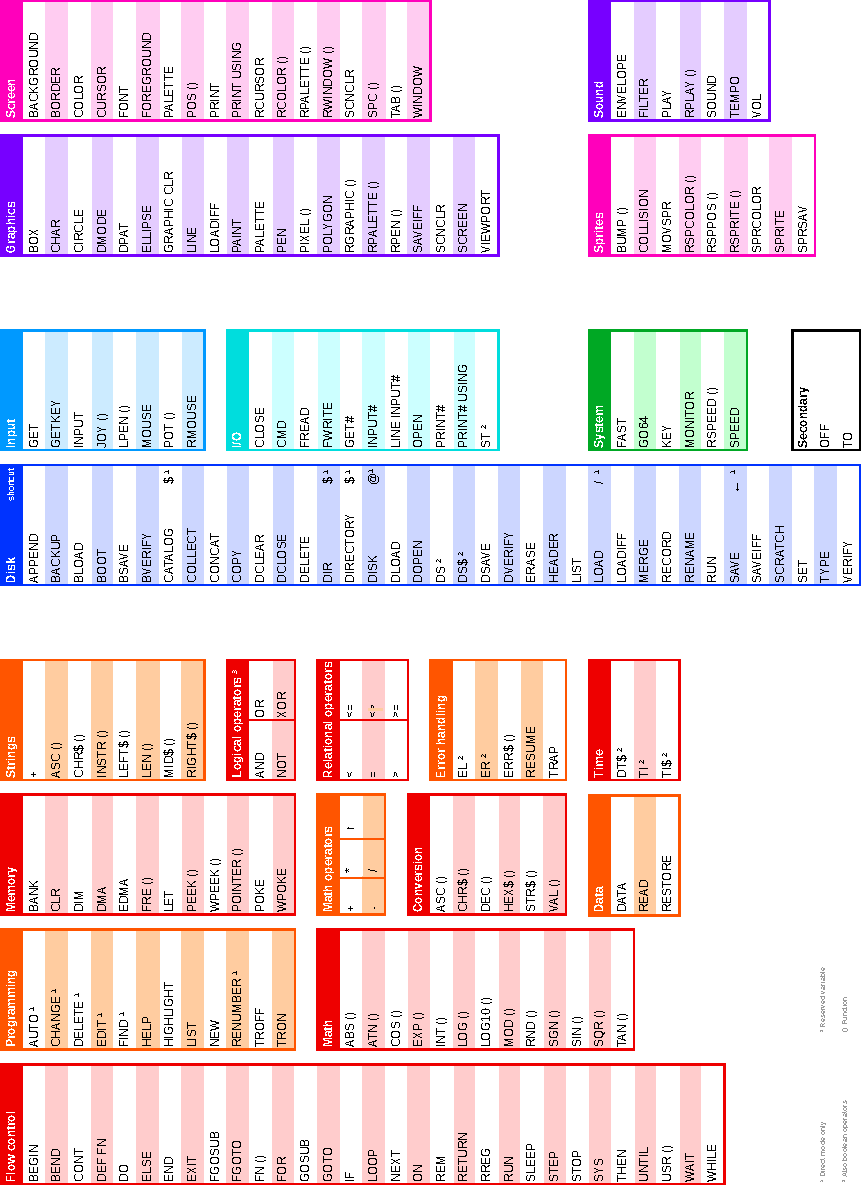
\includegraphics[width=\linewidth]{images/illustrations/basic65_quick_reference_card.pdf}
% Landscape orientation of Quick Reference for printing:
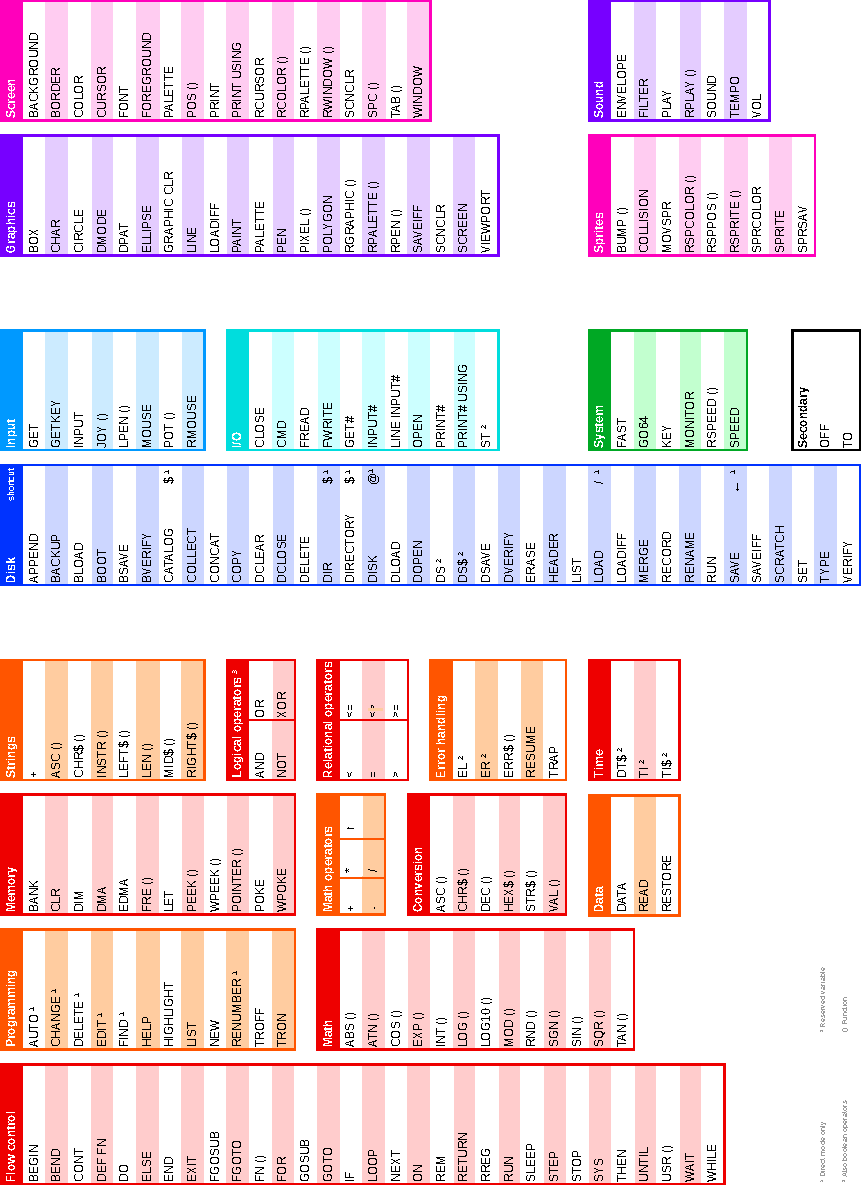
\includegraphics[angle=90,origin=c,height=5.75in]{images/illustrations/basic65_quick_reference_card.pdf}

\newpage
\begin{tikzpicture}[remember picture,overlay,shift={(current page.north east)}]
\node[anchor=north east,xshift=0.2cm,yshift=0.1cm]{\includegraphics[height=210mm,width=149mm]{images/manual_back_cover}};
\end{tikzpicture}

\begin{center}

\textbf{\large\textcolor{white}{MEGA Museum of Electronic Games \& Art e.V. \\
\vspace{3mm}
\url{http://mega65.org}}}\\
\vspace{6mm}
\textbf{\large\textcolor{white}{
Editors:\\
\vspace{2mm}
Dr. Paul Gardner-Stephen\\
Dr. Edilbert Kirk\\
\vspace{6mm}
Authors: \\
\vspace{2mm}
Dr. Paul Gardner-Stephen\\
Dr. Edilbert Kirk\\
Detlef Hastik\\
Gürçe Işıkyıldız\\
Stephan Kleinert\\
Maurice van Gils\\
Wayne Johnson\\
Daren Klamer\\
Jim Nicholls\\
Oliver Graf\\
Dan Sanderson\\
\vspace{6mm}
and many other contributors\\
}}
\vspace{4.1cm}
\colorbox{white}{\EANisbn[ISBN=978-0-6452968-1-5,SC4]}
\end{center}

\input{common-footer}

